\documentclass[11pt,a4paper]{article}
\usepackage[T1]{fontenc}
\usepackage{calligra}
\usepackage{makeidx}
\usepackage{hyperref}
\usepackage{amsmath}
\usepackage{amsfonts}
\usepackage{amssymb}
\usepackage{makeidx}
\usepackage{graphicx}
\usepackage{wrapfig}
\usepackage{amsmath}
\usepackage{enumerate}
\usepackage{subfigure}
\usepackage{fancyhdr}
\usepackage{amsthm}
\usepackage{amsfonts}
\usepackage{slashed}

\usepackage[a4paper, inner=1.5cm, outer=3cm, top=3cm, 
bottom=3cm, bindingoffset=1cm]{geometry} 

\begin{document}
\title{Numerical solution of the avvection equation using finite difference methods} 
\author{Simone Orioli} 
\date{Academic Year 2013/2014} 
\maketitle

\renewcommand{\thesubfigure}{\thefigure.\arabic{subfigure}}
\makeatletter
\renewcommand{\@thesubfigure}{\thesubfigure:\space}
\renewcommand{\p@subfigure}{}
\makeatother
\setcounter{lofdepth}{2}

\section{Introduction}
\emph{Given the advection equation in 1D $u_t+u_x=0$ build a numerical code to solve it on a grid with extent $x\in [0,10]$ and with initial conditions given by}
\begin{equation}\label{1.1}
u(x,t=0) = \exp [ -(x-x_0)^2]
\end{equation}
\emph{with $x_0=5$, or}
\begin{equation}\label{1.2}
u(x,t=0) = \begin{cases}
1 \text{ }\text{ if } x \in [4,6] \\
0 \text{ }\text{ otherwise}
\end{cases}
\end{equation}
\emph{Perform the time integration using the following schemes:
\begin{enumerate}
\item FTCS;
\item Lax-Friedrichs;
\item Leapfrog;
\item Lax-Wendroff.
\end{enumerate}
Use Courant factors $c_f=0.5$ and $c_f=1$ and compare the results obtained with the different methods, paying attention to their stability and dissipation properties (e.g., plot $u(x,t)$ at different times and the evolution of the L2-norm). Use at least $J=101$ points in the $x$ direction, so that the spacing $\delta x$ is at least $0.1$, and terminate your simulation at $t=20$. Use periodic boundary conditions.} \\
%\begin{figure}[!h]
%\centering
%\subfigure[Plot of \eqref{1.1}]
%{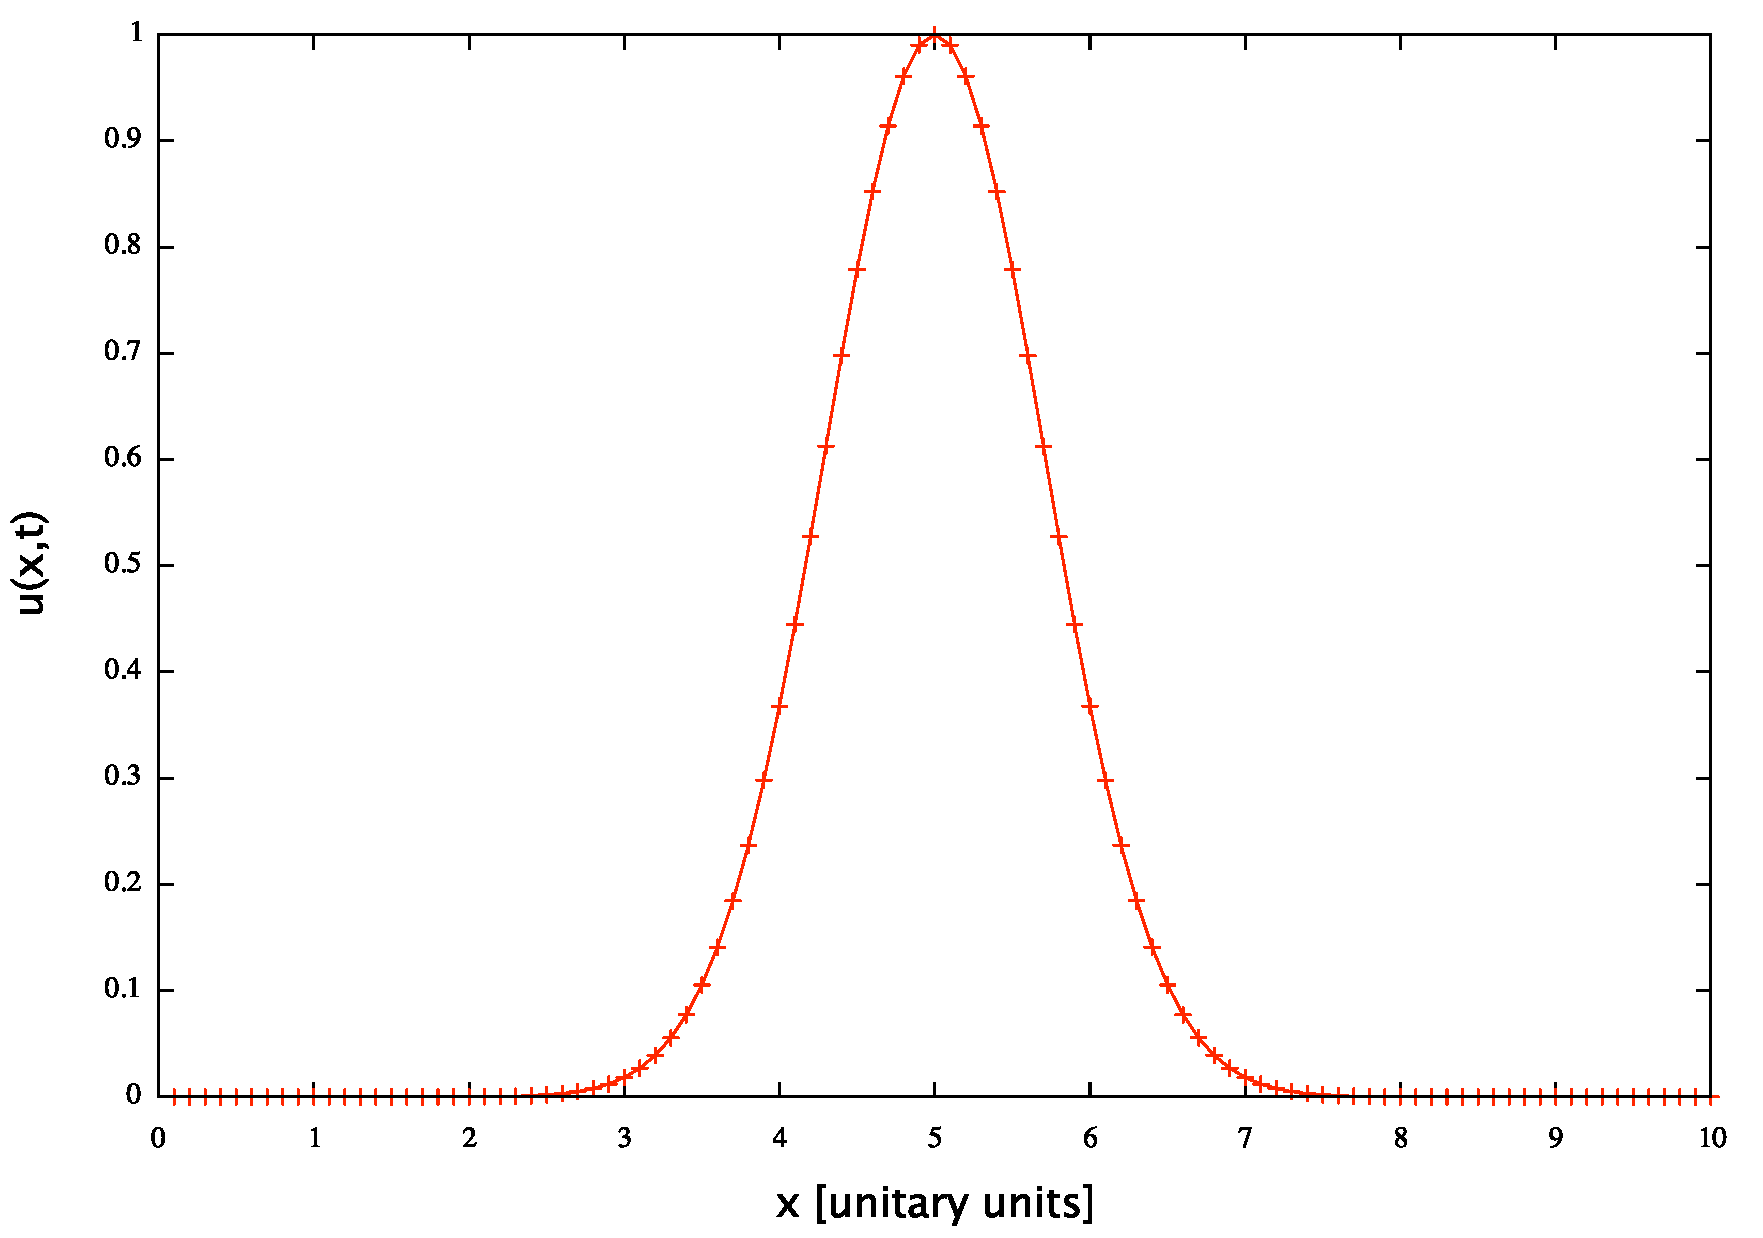
\includegraphics[scale=0.25]{gauss}}
%\hspace{5mm}
%\subfigure[Plot of \eqref{1.2}]
%{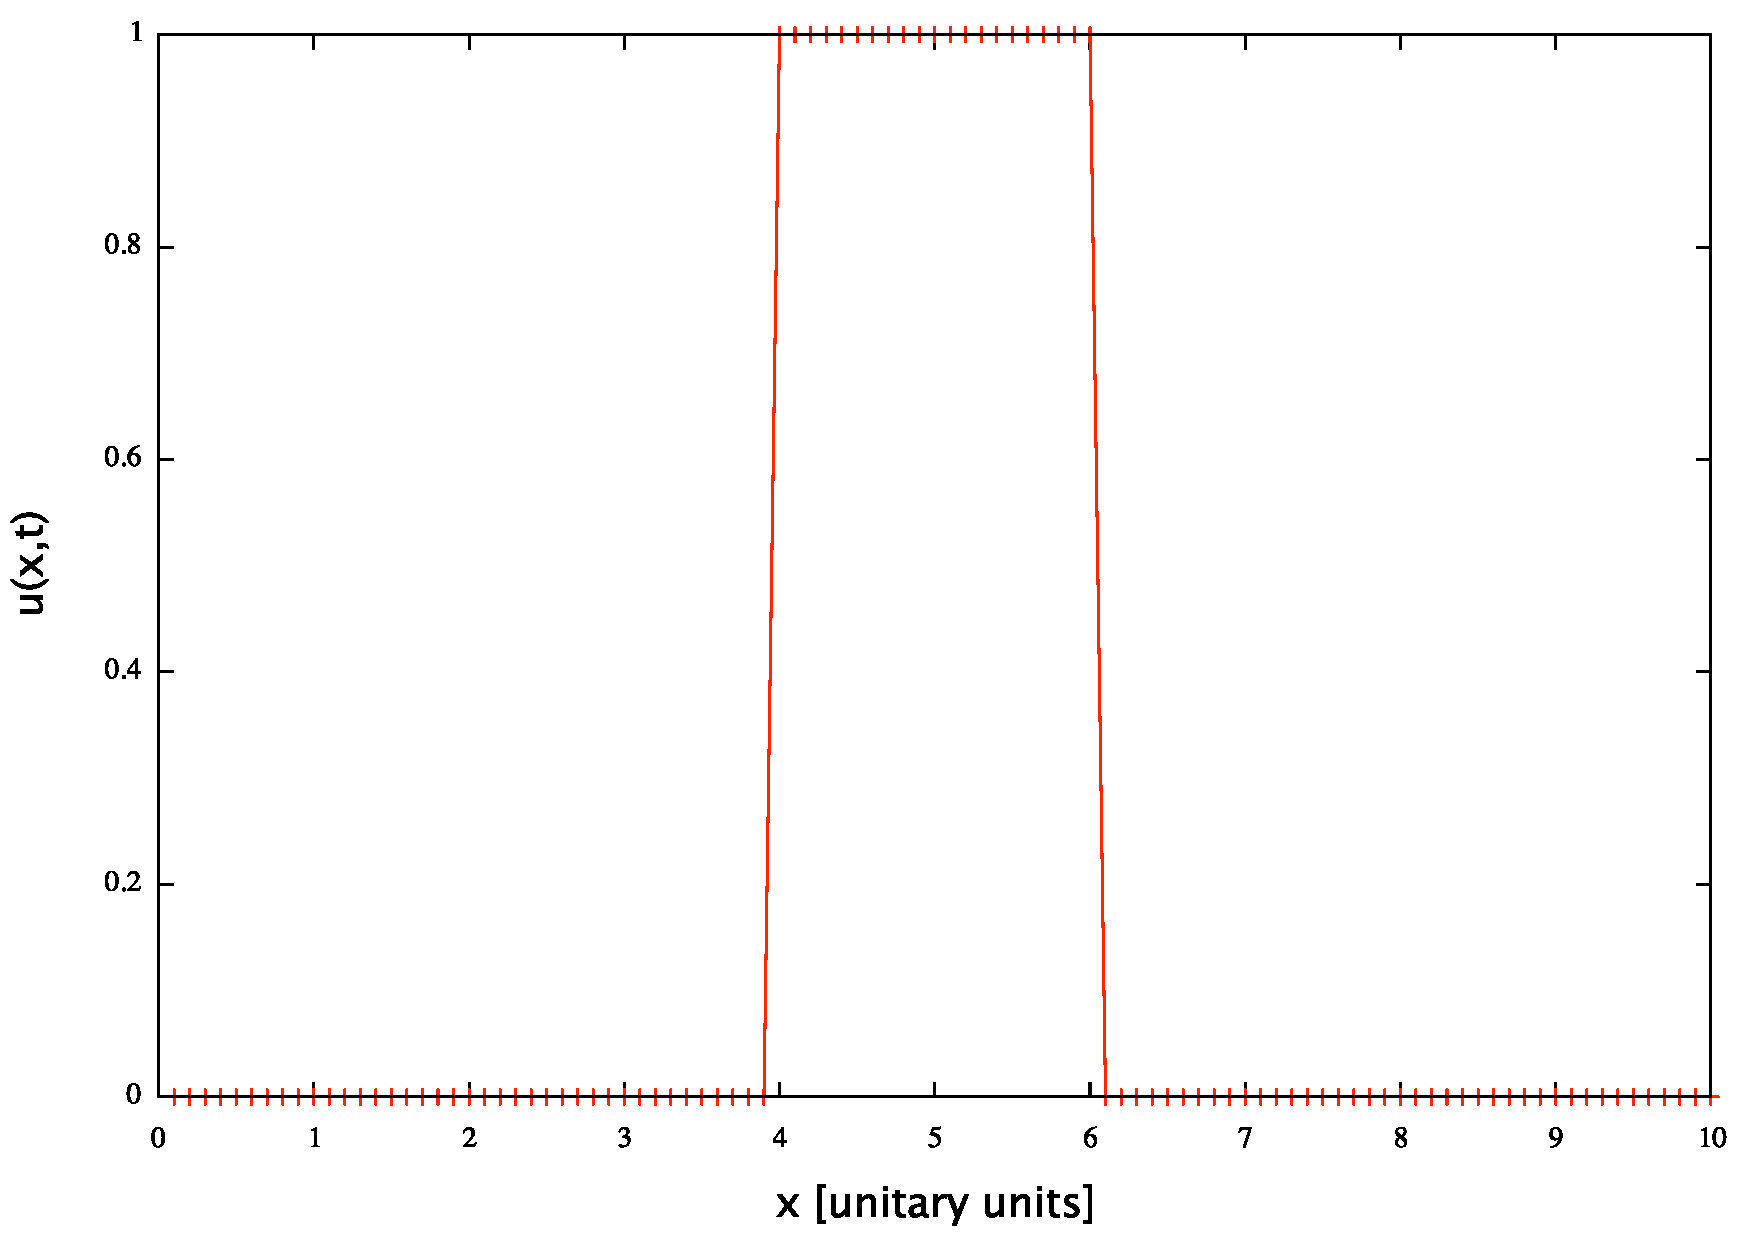
\includegraphics[scale=0.25]{sw}}
%\end{figure}\ \\

We give now some basic information and definitions that will be useful in the following sections. First of all, in discussing the algorithms used to solve the advection equation, the following notation will be used:
\begin{equation}
u_j^n \equiv u(x_j,t^n)
\end{equation}
Secondary, the periodic boundary conditions are given by the following relations:
\begin{equation}
\begin{cases}
u_0^n = u_J^n \\
u^n_{J+1}=u_1^n \\
\end{cases}
\end{equation}
while the L2-norm is defined as
\begin{equation}
||u^n_j||_2 \equiv \sqrt{\frac{1}{J}\sum_{i=1}^J |u_j^n|^2}
\end{equation}
Once chosen the space step $\Delta x$, the time step has always been obtained using the \emph{CFL-condition}:
\begin{equation}
\Delta t = c_f \frac{\Delta x}{|a|}
\end{equation}
where, in our particular case, $|a|=1$, and $c_f$ is the Courant factor that has to obey the constraint $c_f \leq 1$. 
\section{The FTCS method}
The FTCS method (\emph{Forward in Time Centered in Space}) is a first order method in time and a second order method in space, based on the following algorithm:
\begin{equation}
u_j^{n+1} = u_j^n - a\frac{\Delta t}{\Delta x} ( u_{j+1}^n - u_{j-1}^n)
\end{equation}
However, this method is unstable and therefore is useless for simulations which last in time. With the initial condition \eqref{1.1}, the following results are obtained for the evolution of the wave in the case of a $J=101$ (Fig. 1.1 - 1.4):
\begin{figure}[!h]
\centering
\subfigure[$u(x,t=10)$ with $c_f=0.5$]
{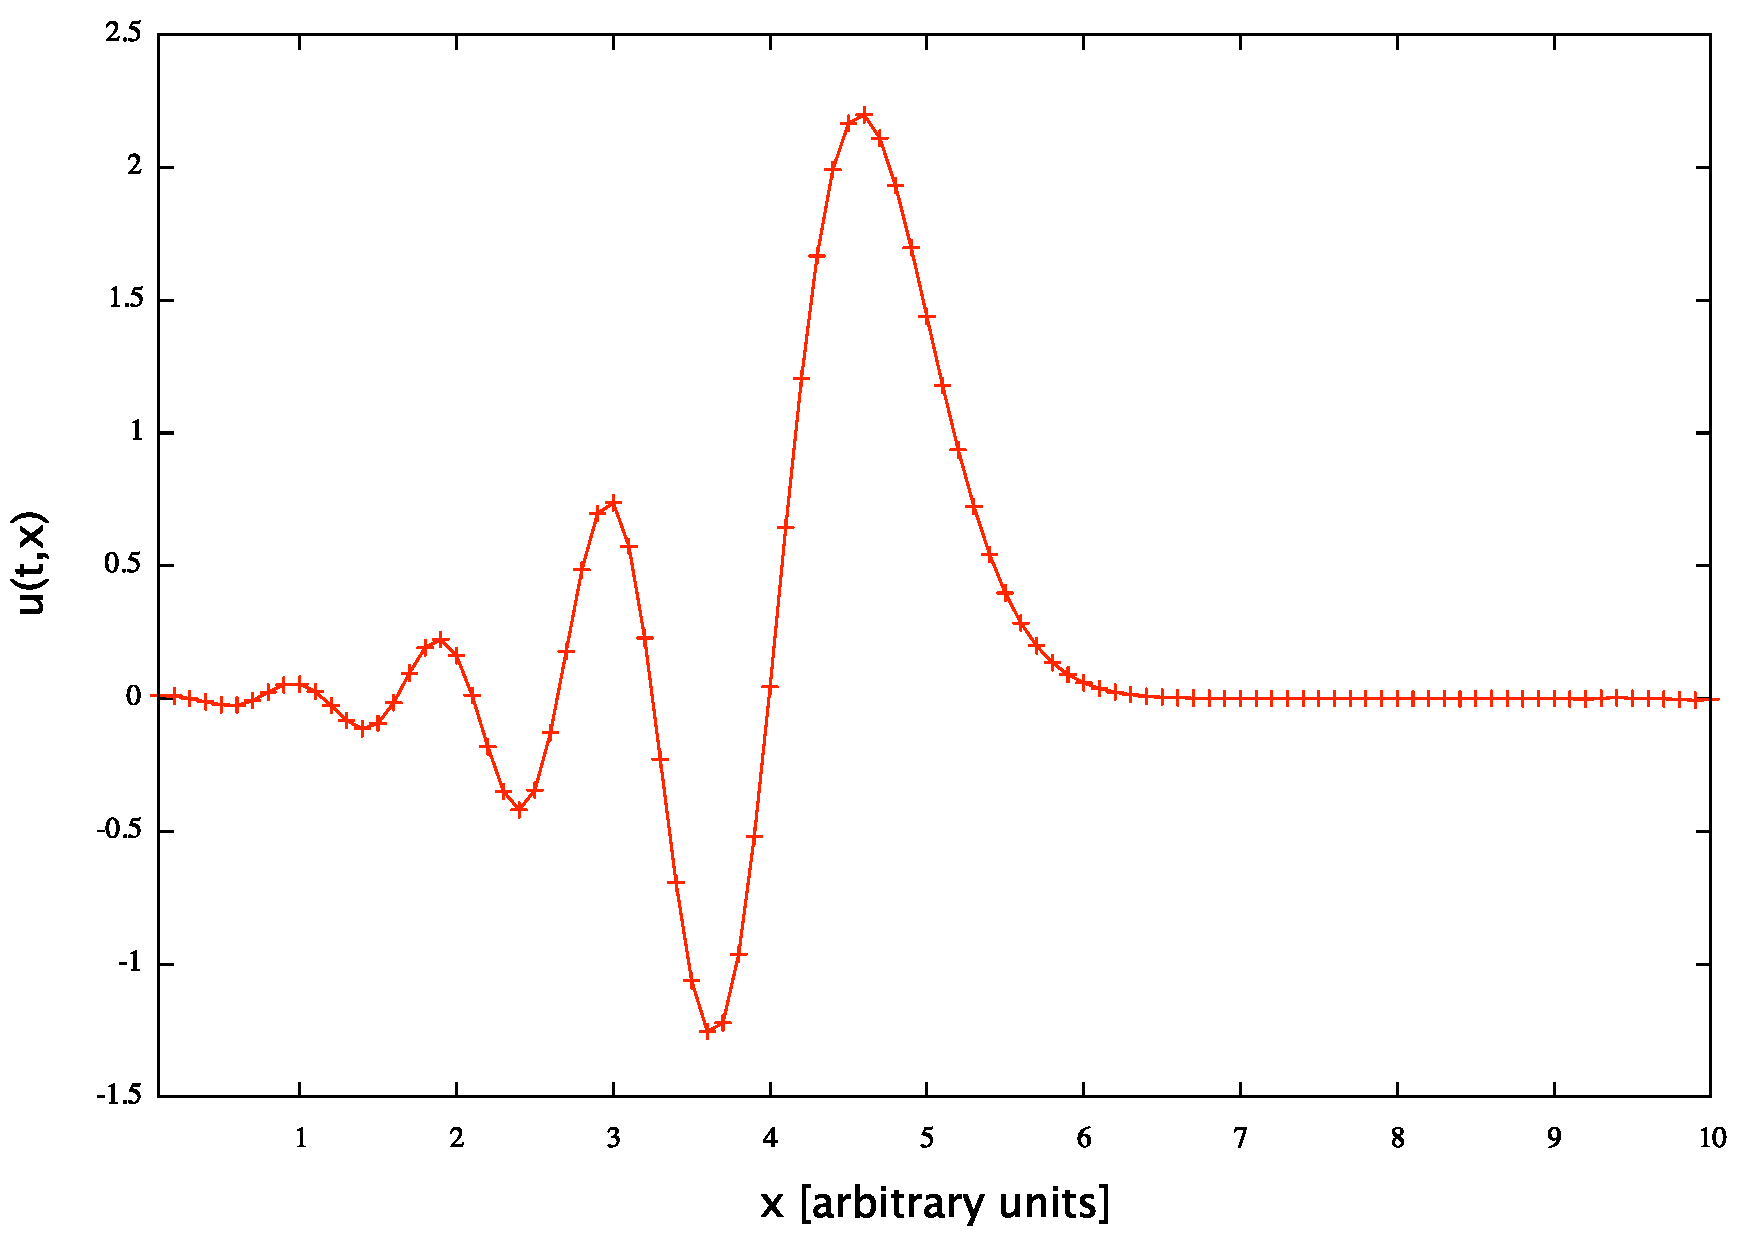
\includegraphics[scale=0.25]{ftcs_t10_cf05}}
\subfigure[$u(x,t=20)$ with $c_f=0.5$]
{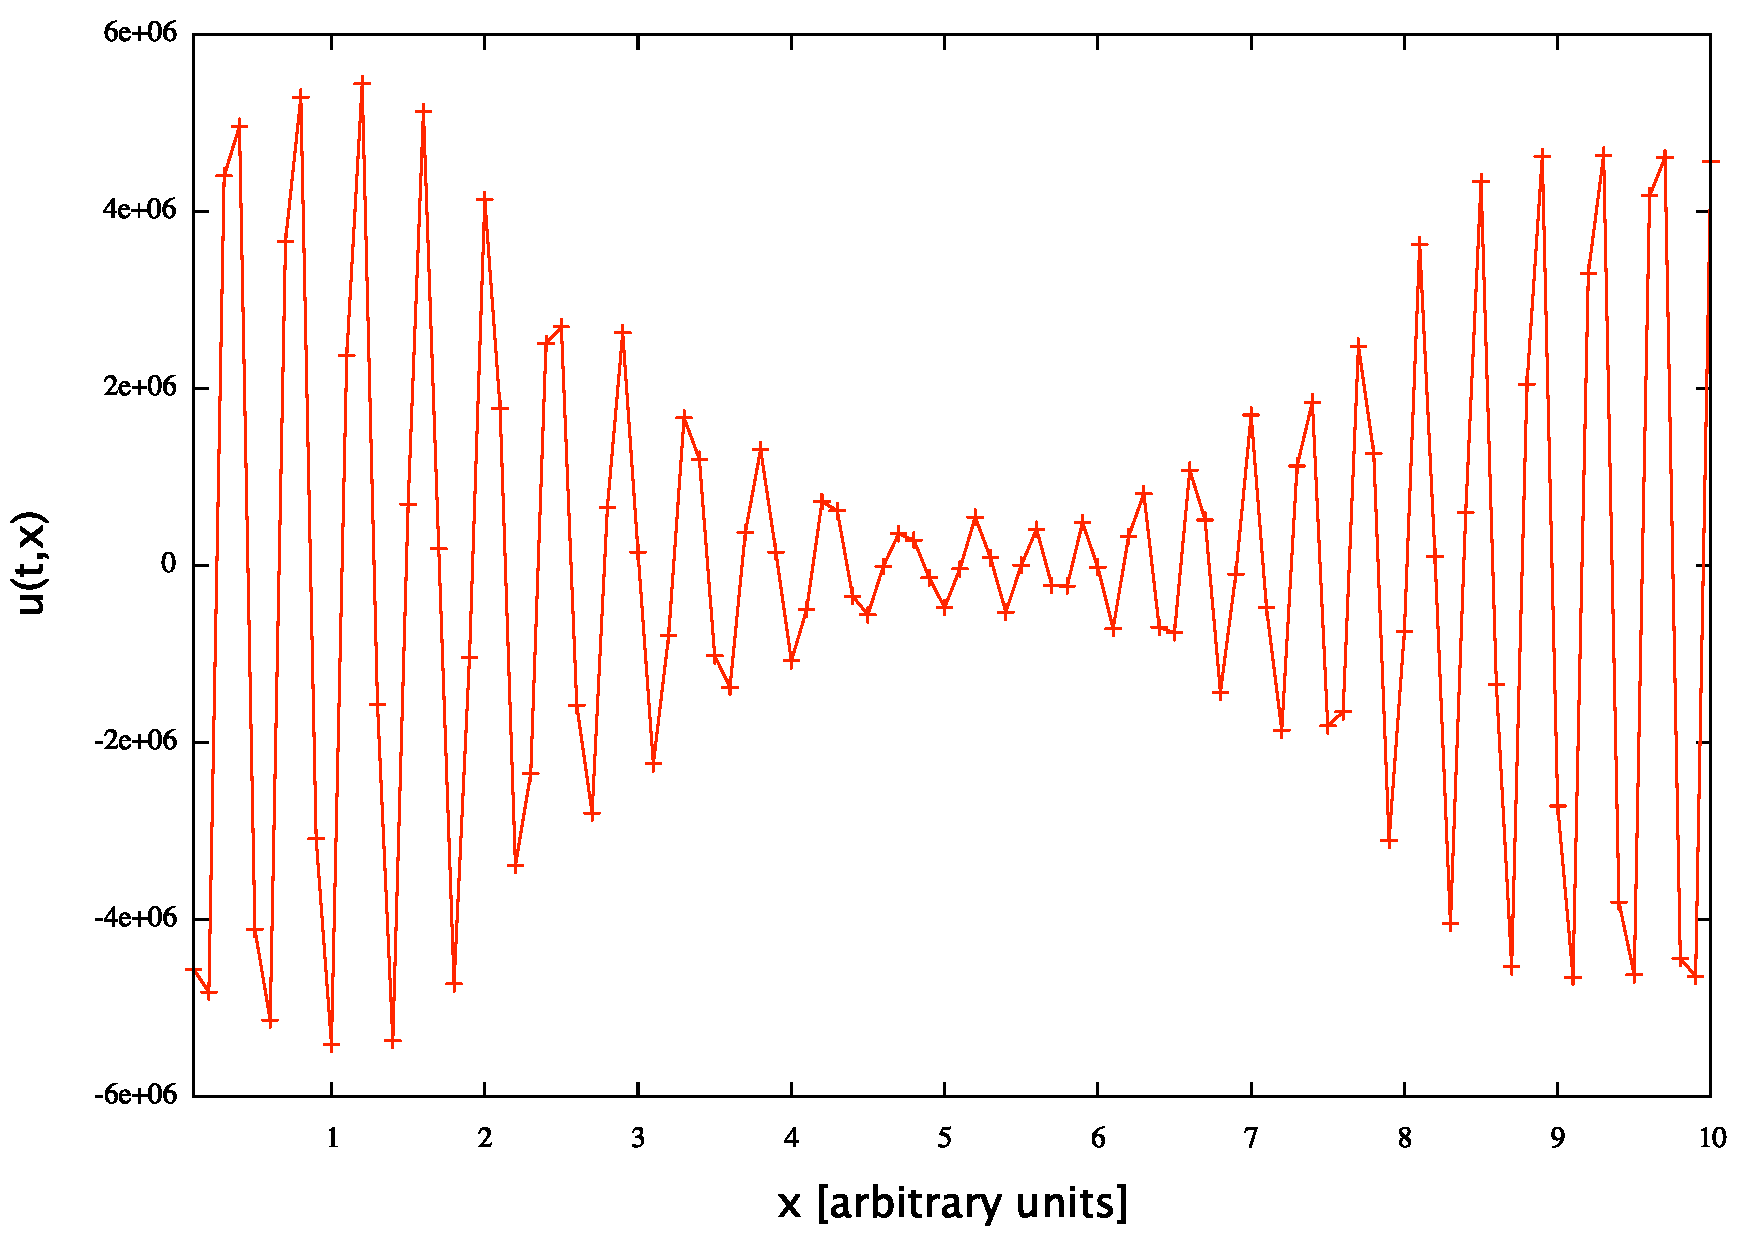
\includegraphics[scale=0.25]{ftcs_t20_cf05}}
\subfigure[$u(x,t=10)$ with $c_f=1$]
{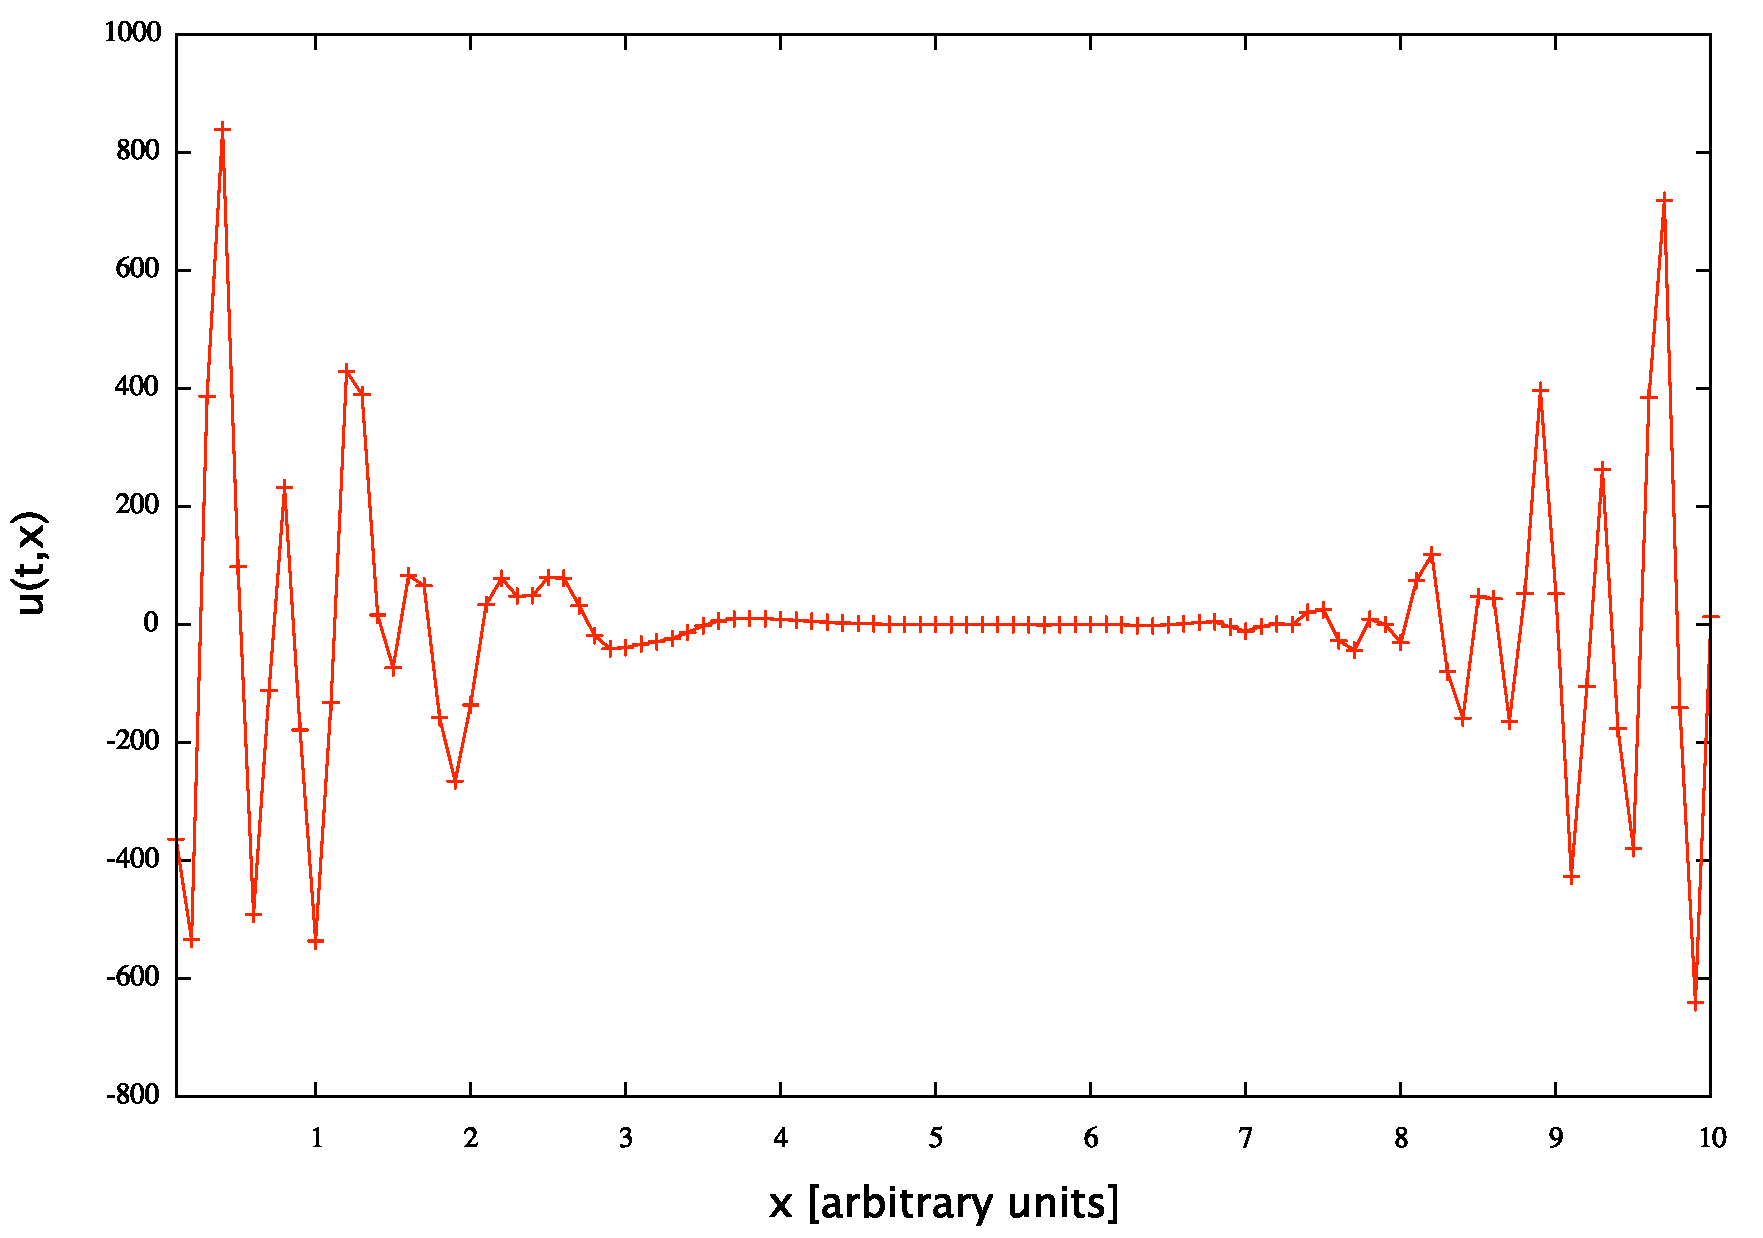
\includegraphics[scale=0.25]{ftcs_t10_cf1}}
\subfigure[$u(x,t=20)$ with $c_f=1$]
{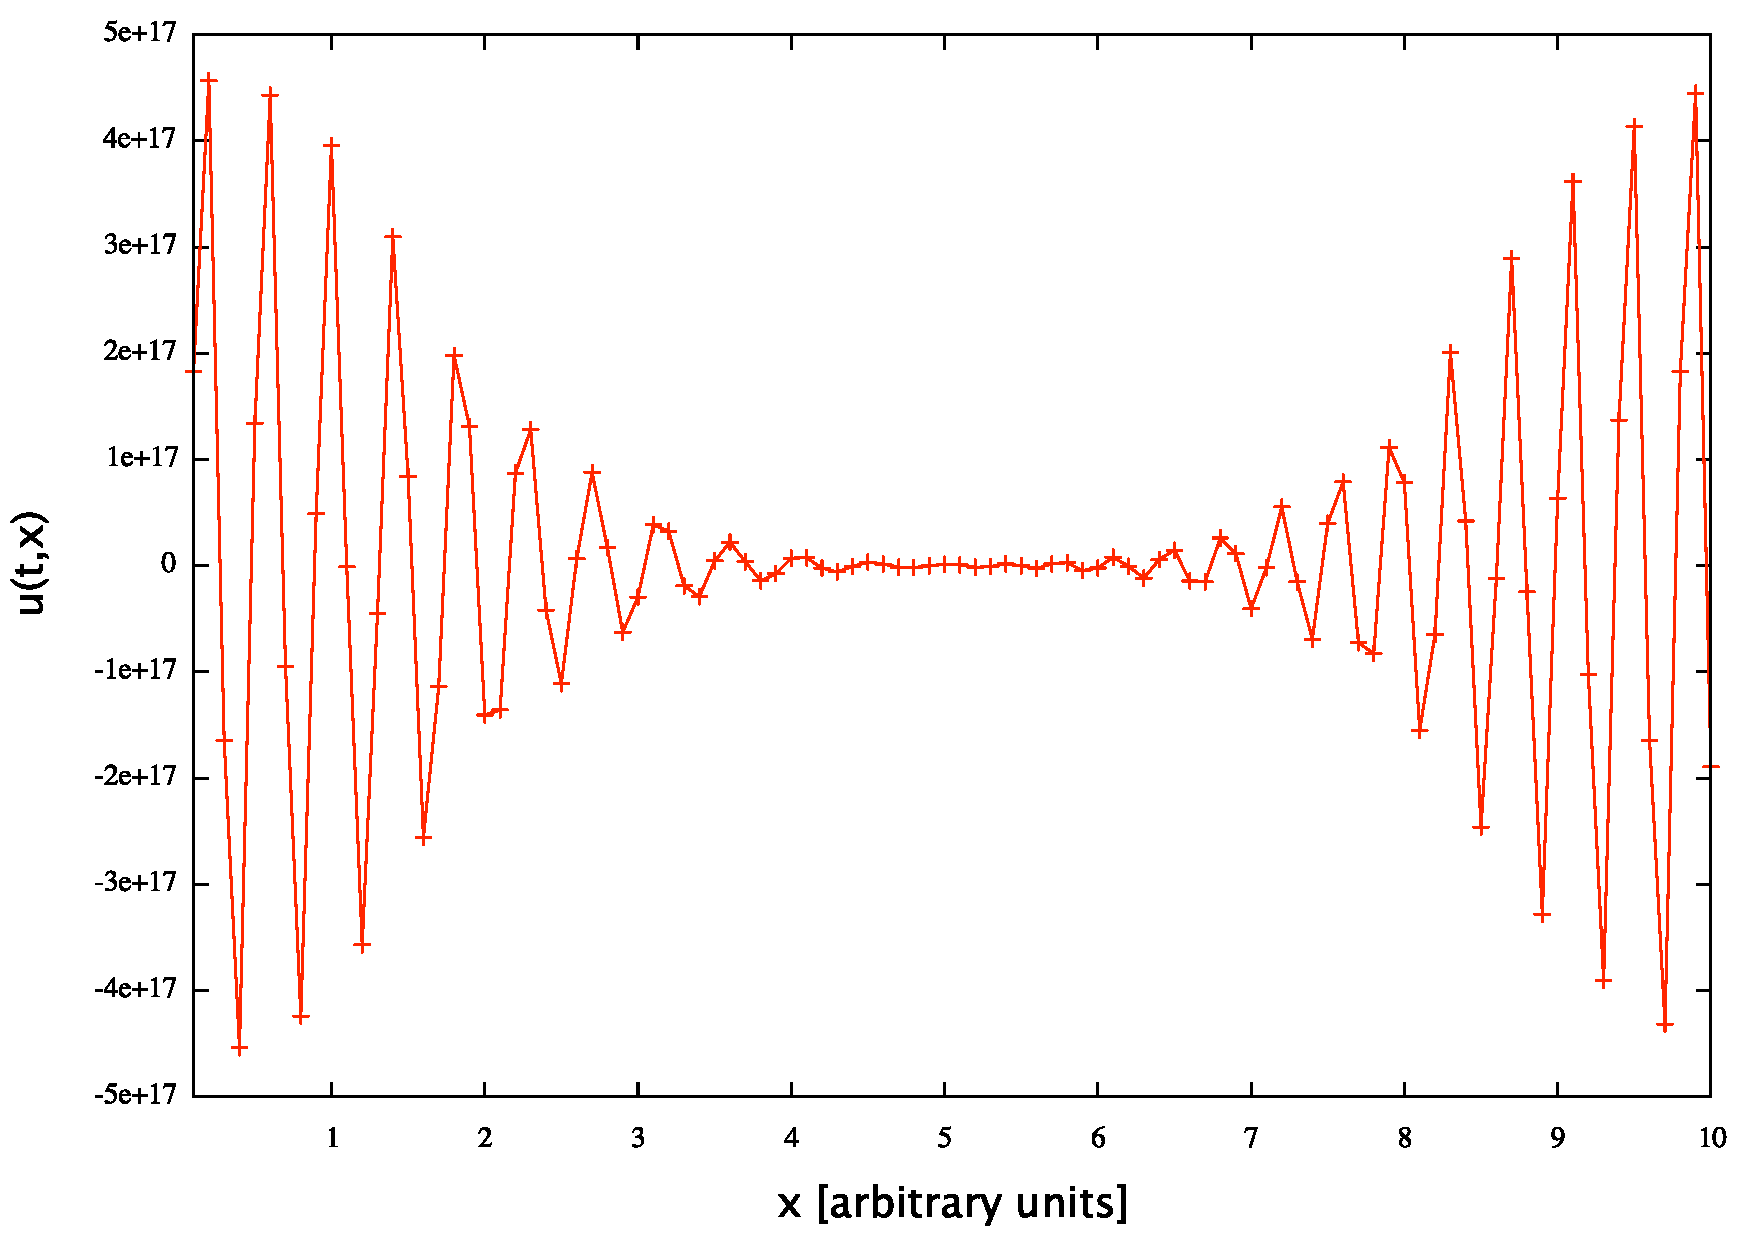
\includegraphics[scale=0.25]{ftcs_t20_cf1}}
\end{figure} \ \\ \\
%In the case of $J=101$ points in the grid and $c_f=1$, instead, the following results are obtained:
%\begin{figure}[!h]
%\centering
%\caption{Results obtained with a gaussian wave with $J=101$ and $c_f=1$ using FTCS}
%\end{figure}\ \\ \\
As one can easily figure out from the plots, the instability of the method completely destroys the solution even within $t=10$, which means that the method is quite useless for long lasting time evolutions, as initially stated. Different solutions of the avvection equation can be obtained using as starting function \eqref{1.2} (Fig. 1.5, 1.6). As can be clearly seen from the  plots, the solution is already destroyed within the very first seconds of the simulation. 
\begin{figure}[!h]
\centering
\subfigure[$u(x,t=0.05)$ with $c_f=0.5,1$]
{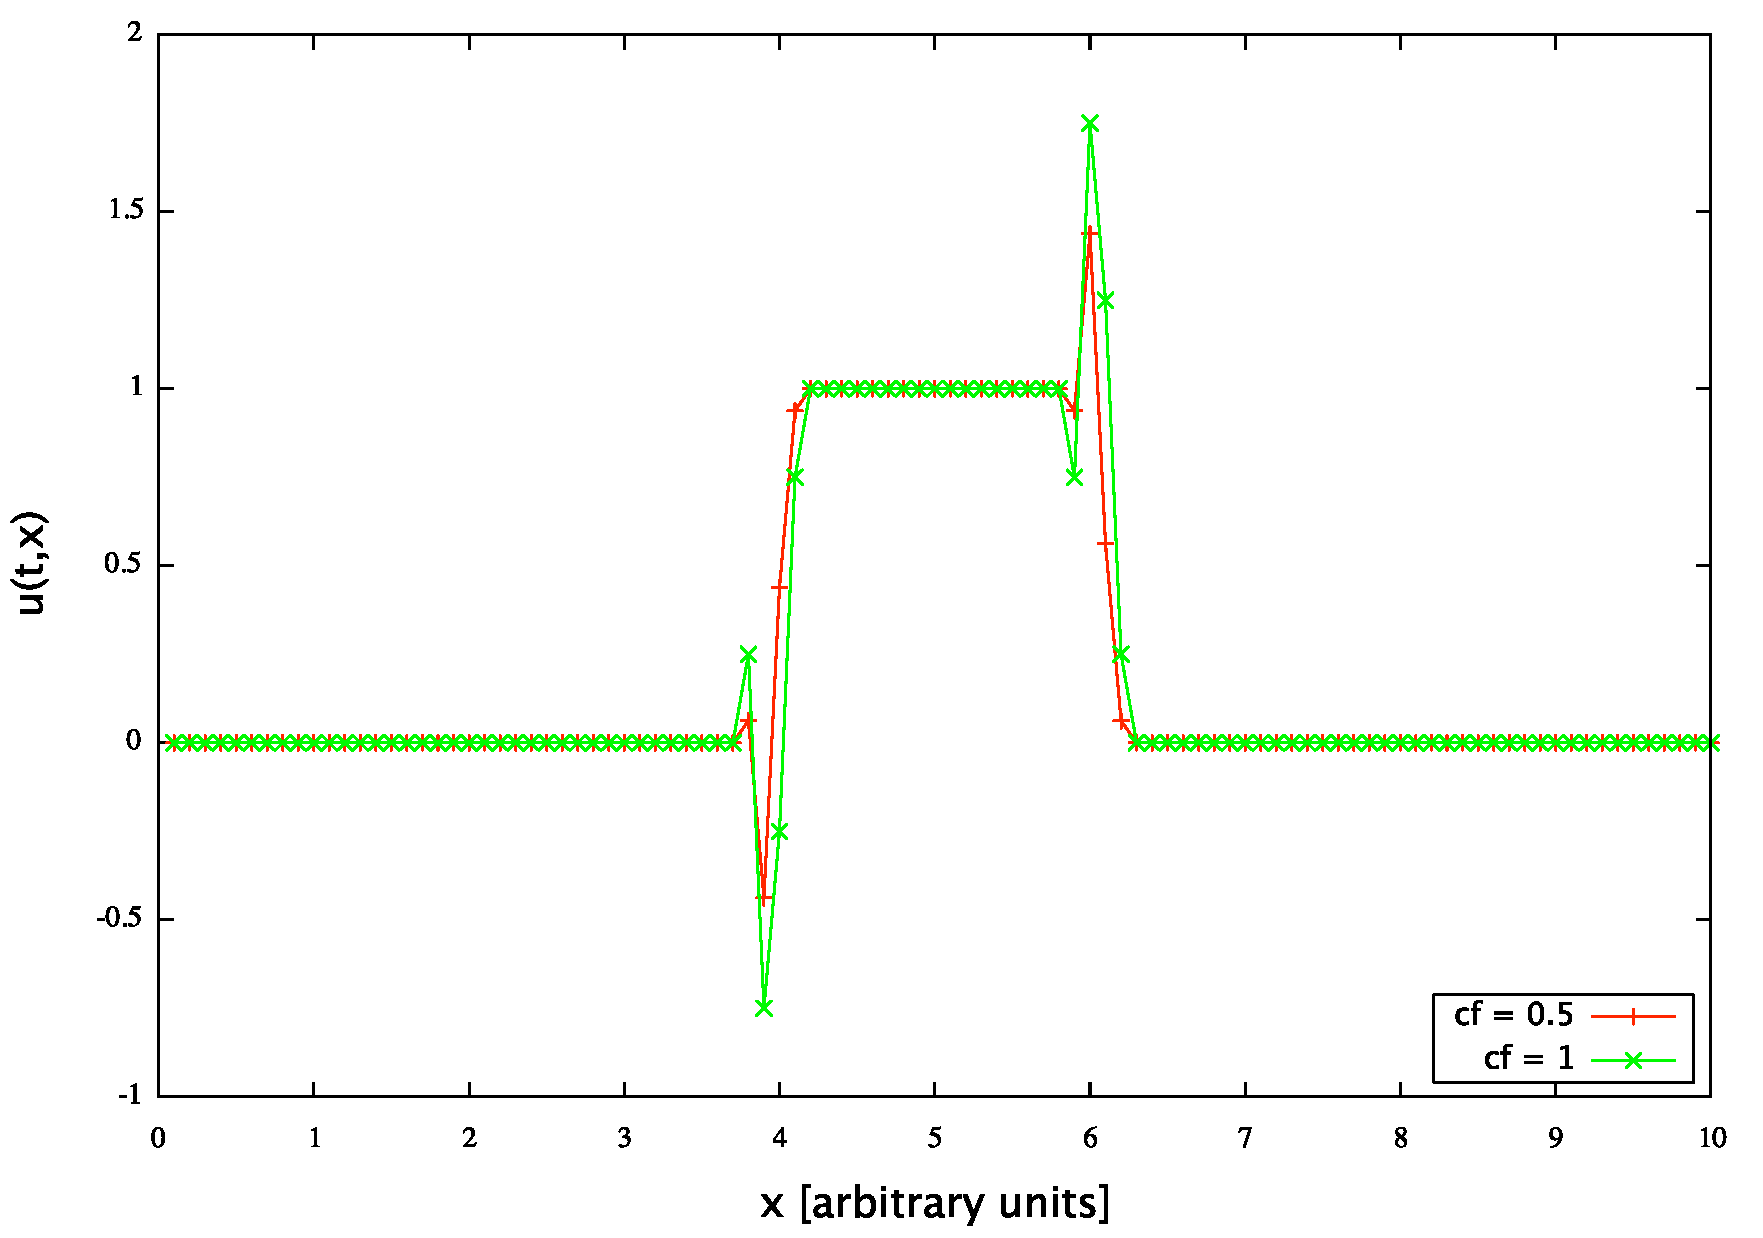
\includegraphics[scale=0.25]{ftcs_sw_tTSTEP}}
\subfigure[$u(x,t=1)$ with $c_f=0.5,1$]
{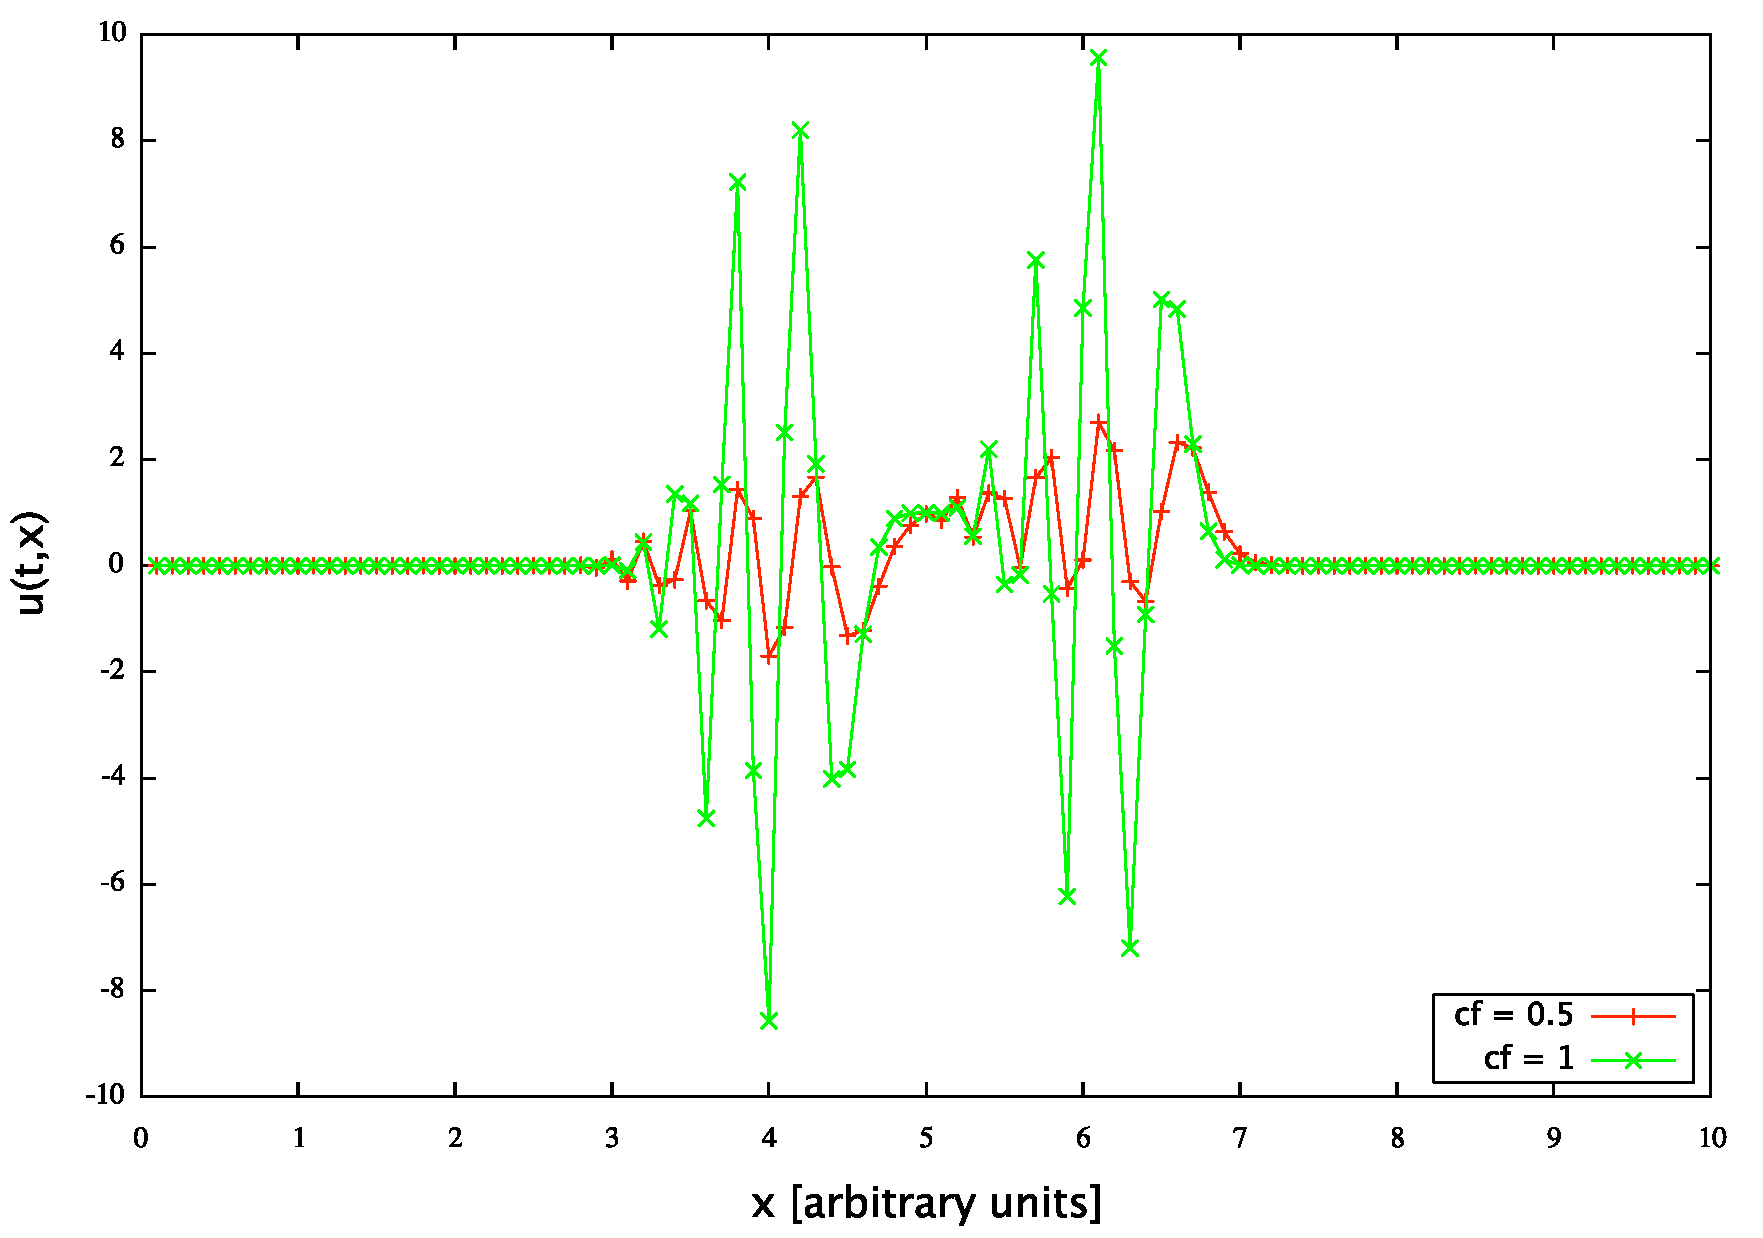
\includegraphics[scale=0.25]{ftcs_t1_sw}}
%\caption{Results obtained with a rectangular wave with $J=101$ and $c_f=0.5,1$ using FTCS}
\end{figure}
In the following we show the plot of the L2-norms in logscale (Fig. 1.7, 1.8). 
\begin{figure}[!h]
\centering
\subfigure[L2-norm with $c_f=0.5,1$ and $\Delta x = 0.1$ for the Gaussian initial condition]
{\includegraphics[scale=0.25]{L2norm_ftcs}}
\subfigure[L2-norm with $c_f=0.5,1$ and $\Delta x = 0.1$ for the square wave initial condition]
{\includegraphics[scale=0.25]{L2norm_ftcs_sw}}
\end{figure}
One observes that the norm in the case of the gaussian wave is monotonously increasing and that it blows-up for for big $t$'s (with both $c_f=0.5$ and $c_f=1$), that is the error on the solution becomes infinite within a finite time. The value reached by the L2-norm for the square wave case at $t=20$ is even bigger then before, showing, definitively, that the FTCS is a non applicable method for the solution of the avvection equation. 
\section{The Leapfrog method}
\begin{figure}[!h]
\centering
\subfigure[$u(x,t=10)$ with $c_f=0.5$]
{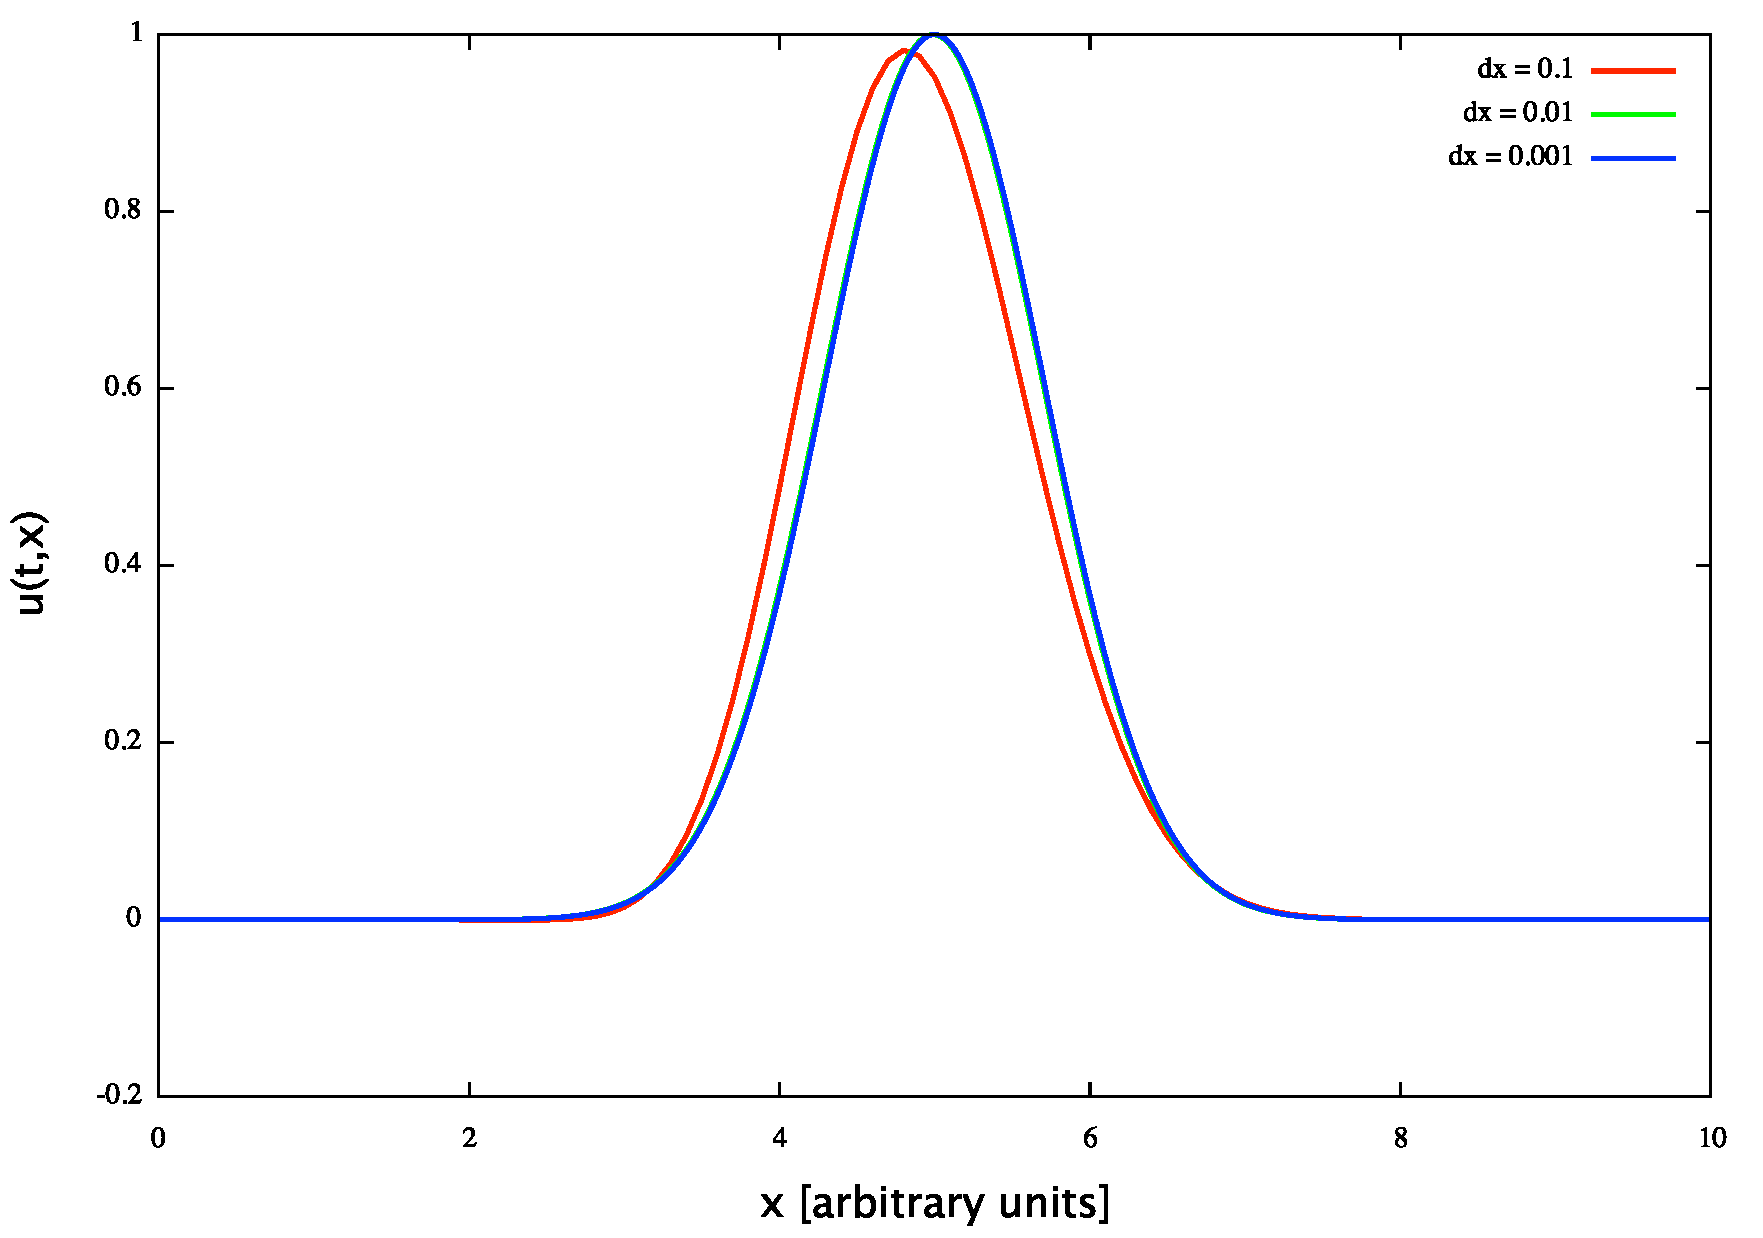
\includegraphics[scale=0.25]{good_img/lf_cf05_t10_g}}
\subfigure[$u(x,t=20)$ with $c_f=0.5$]
{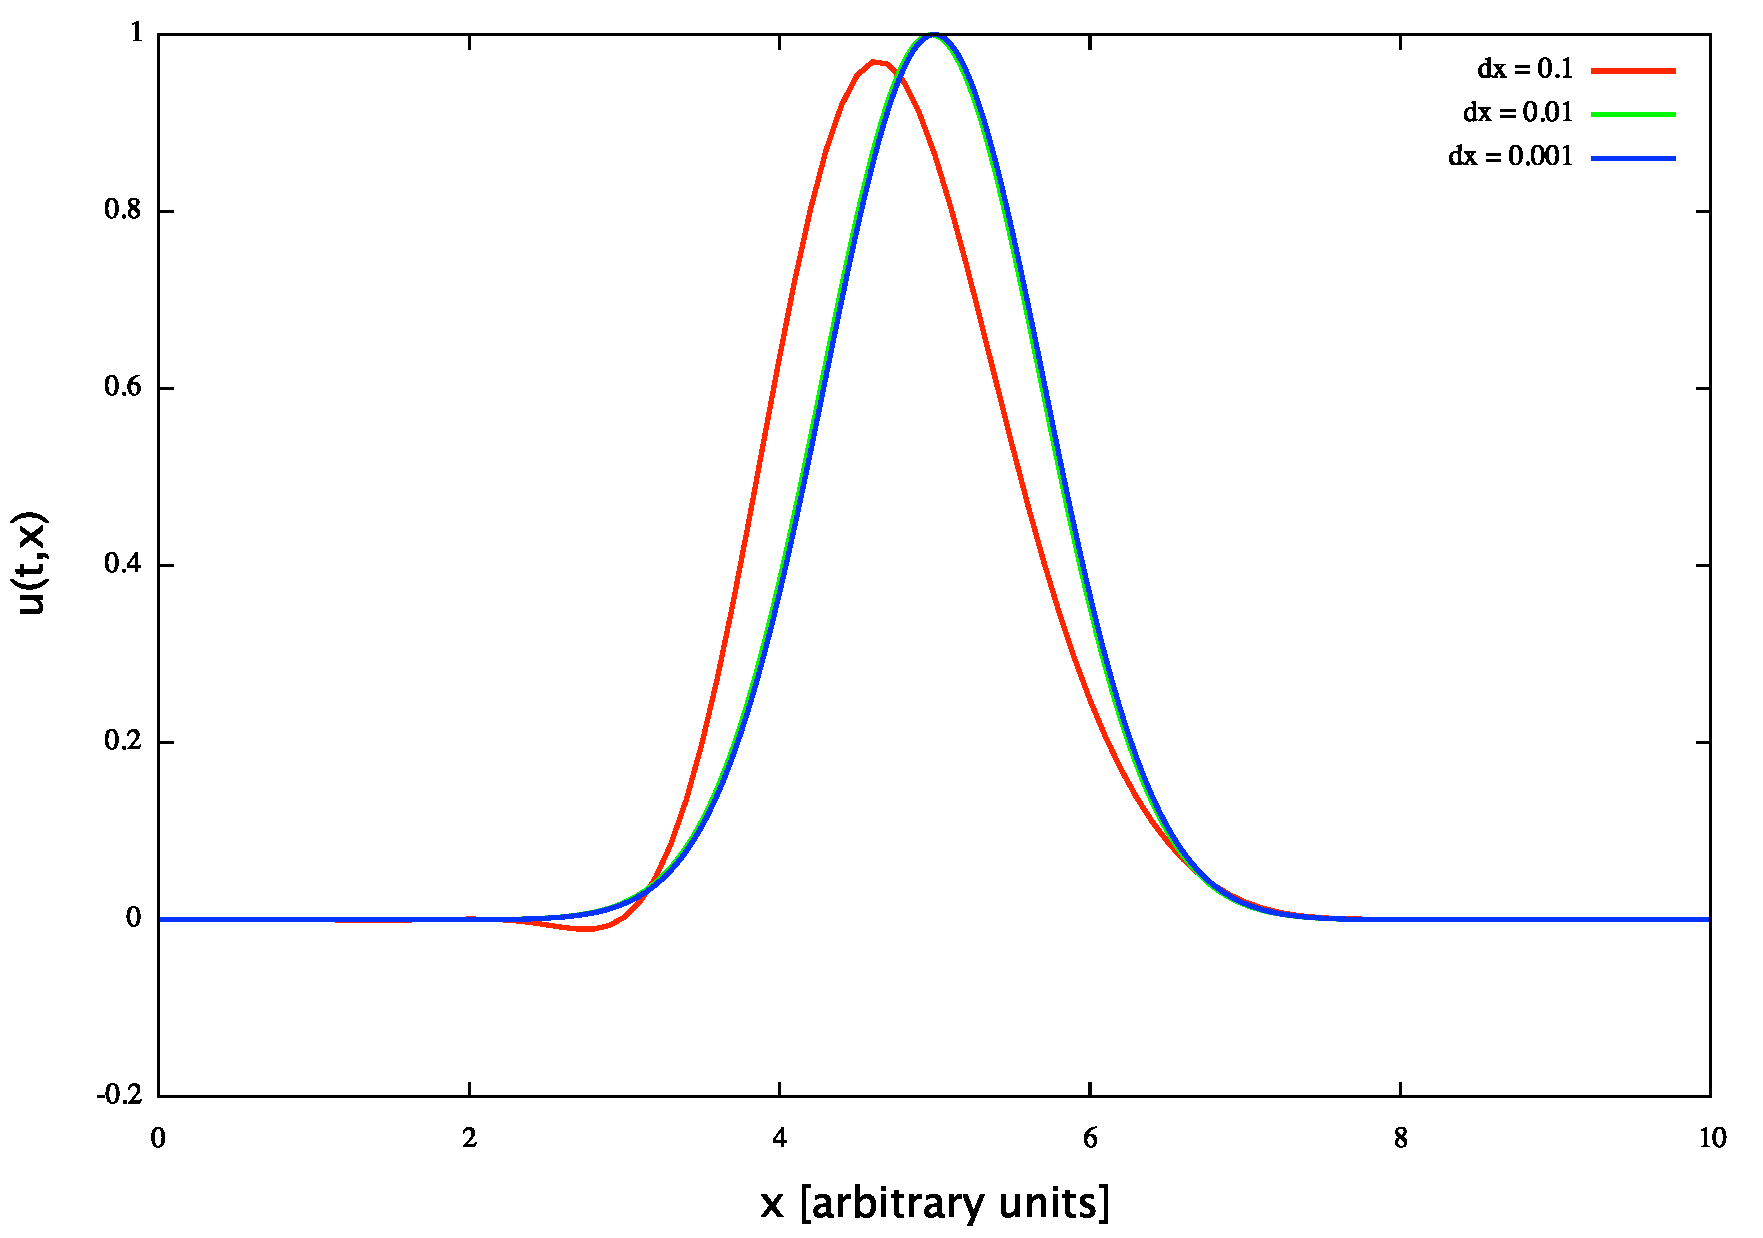
\includegraphics[scale=0.25]{good_img/lf_cf05_t20_g}}
\subfigure[$u(x,t=10)$ with $c_f=1$]
{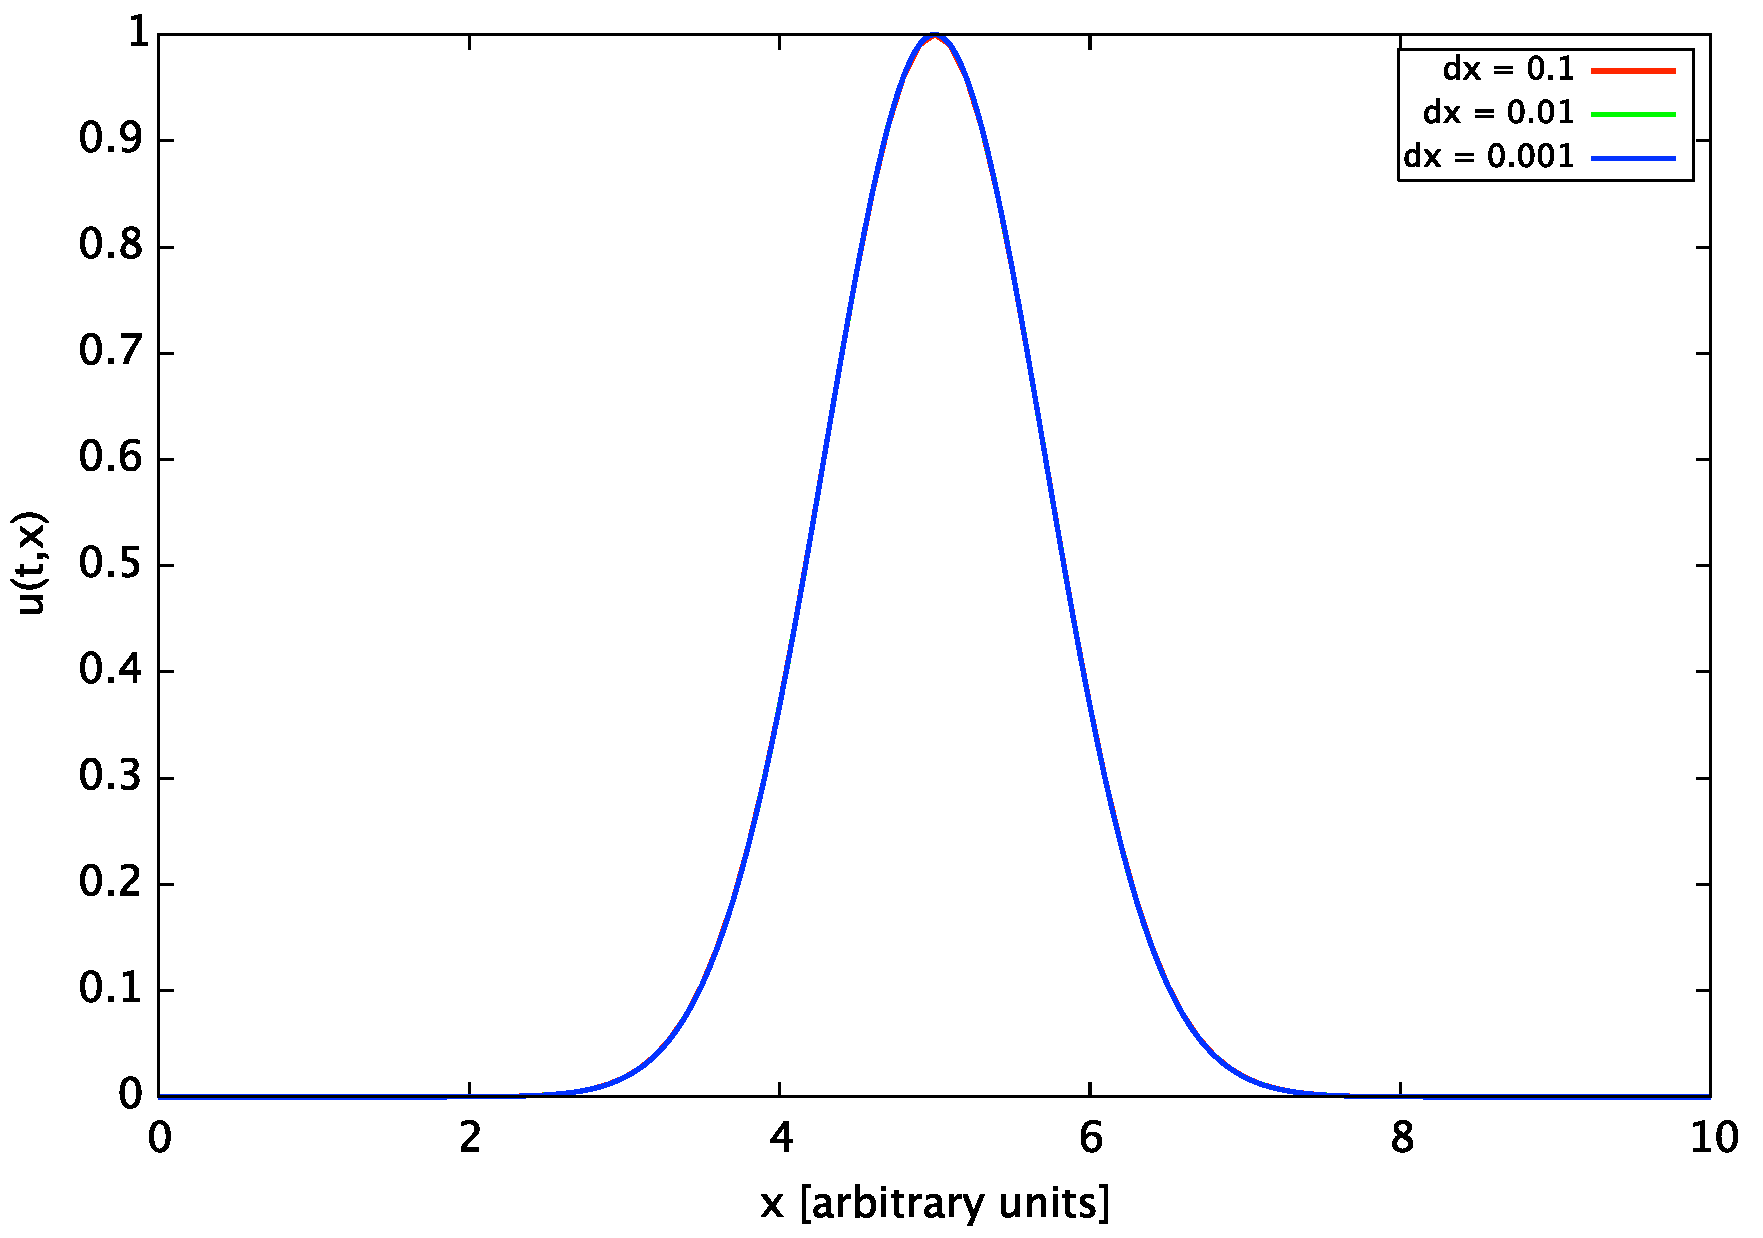
\includegraphics[scale=0.25]{good_img/fig111}}
\subfigure[$u(x,t=20)$ with $c_f=1$]
{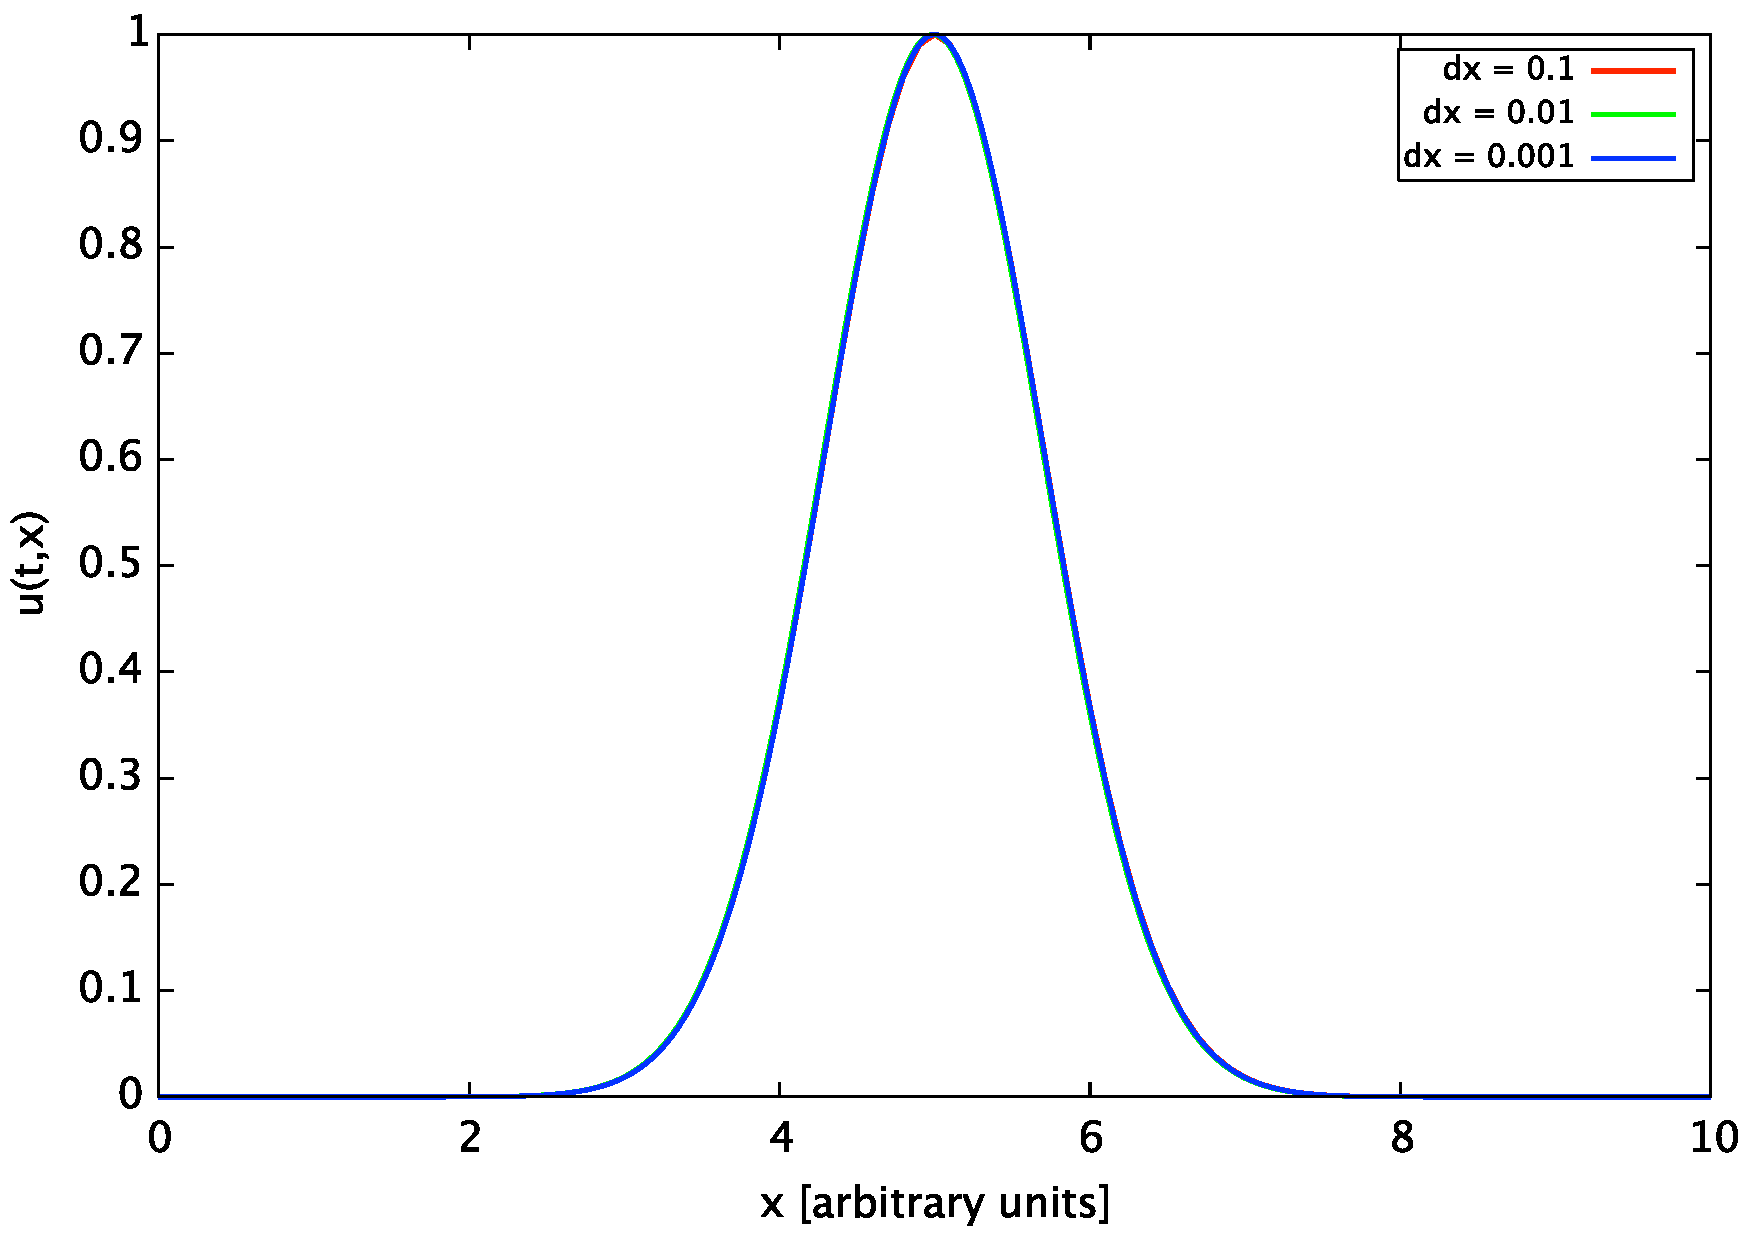
\includegraphics[scale=0.25]{good_img/fig112}}
%\caption{Results obtained with a gaussian wave with $J=101,1001,10001$, $c_f=0.5,1$ and $T = 10,20$ using leapfrog method}
\end{figure}
The \emph{Leapfrog method} states that the solution for the advection equation can be obtained using the following algorithm:
\begin{equation}
u_j^{n+1} = u_j^{n-1} - a\frac{\Delta t}{\Delta x} ( u_{j+1}^n - u_{j-1}^n)
\end{equation}
As can be easily seen, one of the fundamental differences between this and the former method lies in the fact that one needs to double the storage space in order to compute the solution, because the $n+1$ step depends on the $n$ and the $n-1$ steps. Using the Von Neumann stability analysis one finds that leapfrog is a stable method as long as $|a|\frac{\Delta t}{\Delta x} = c_f < 1$. Therefore, let's look at the obtained solutions for initial condition (1) implementing the leapfrog algorithm in different conditions (Fig. 1.9 - 1.12). One sees that the method is indeed stable, and the errors for $J=101$ and $c_f = 0.5$ are only due to the fact that the spacing of the mesh is too big.  About initial condition (2) the different results have been obtained (Fig. 1.13 - 1.16). 
\begin{figure}[!h]
\centering
\subfigure[$u(x,t)$ with $c_f=0.5$ and $\Delta x = 0.1$]
{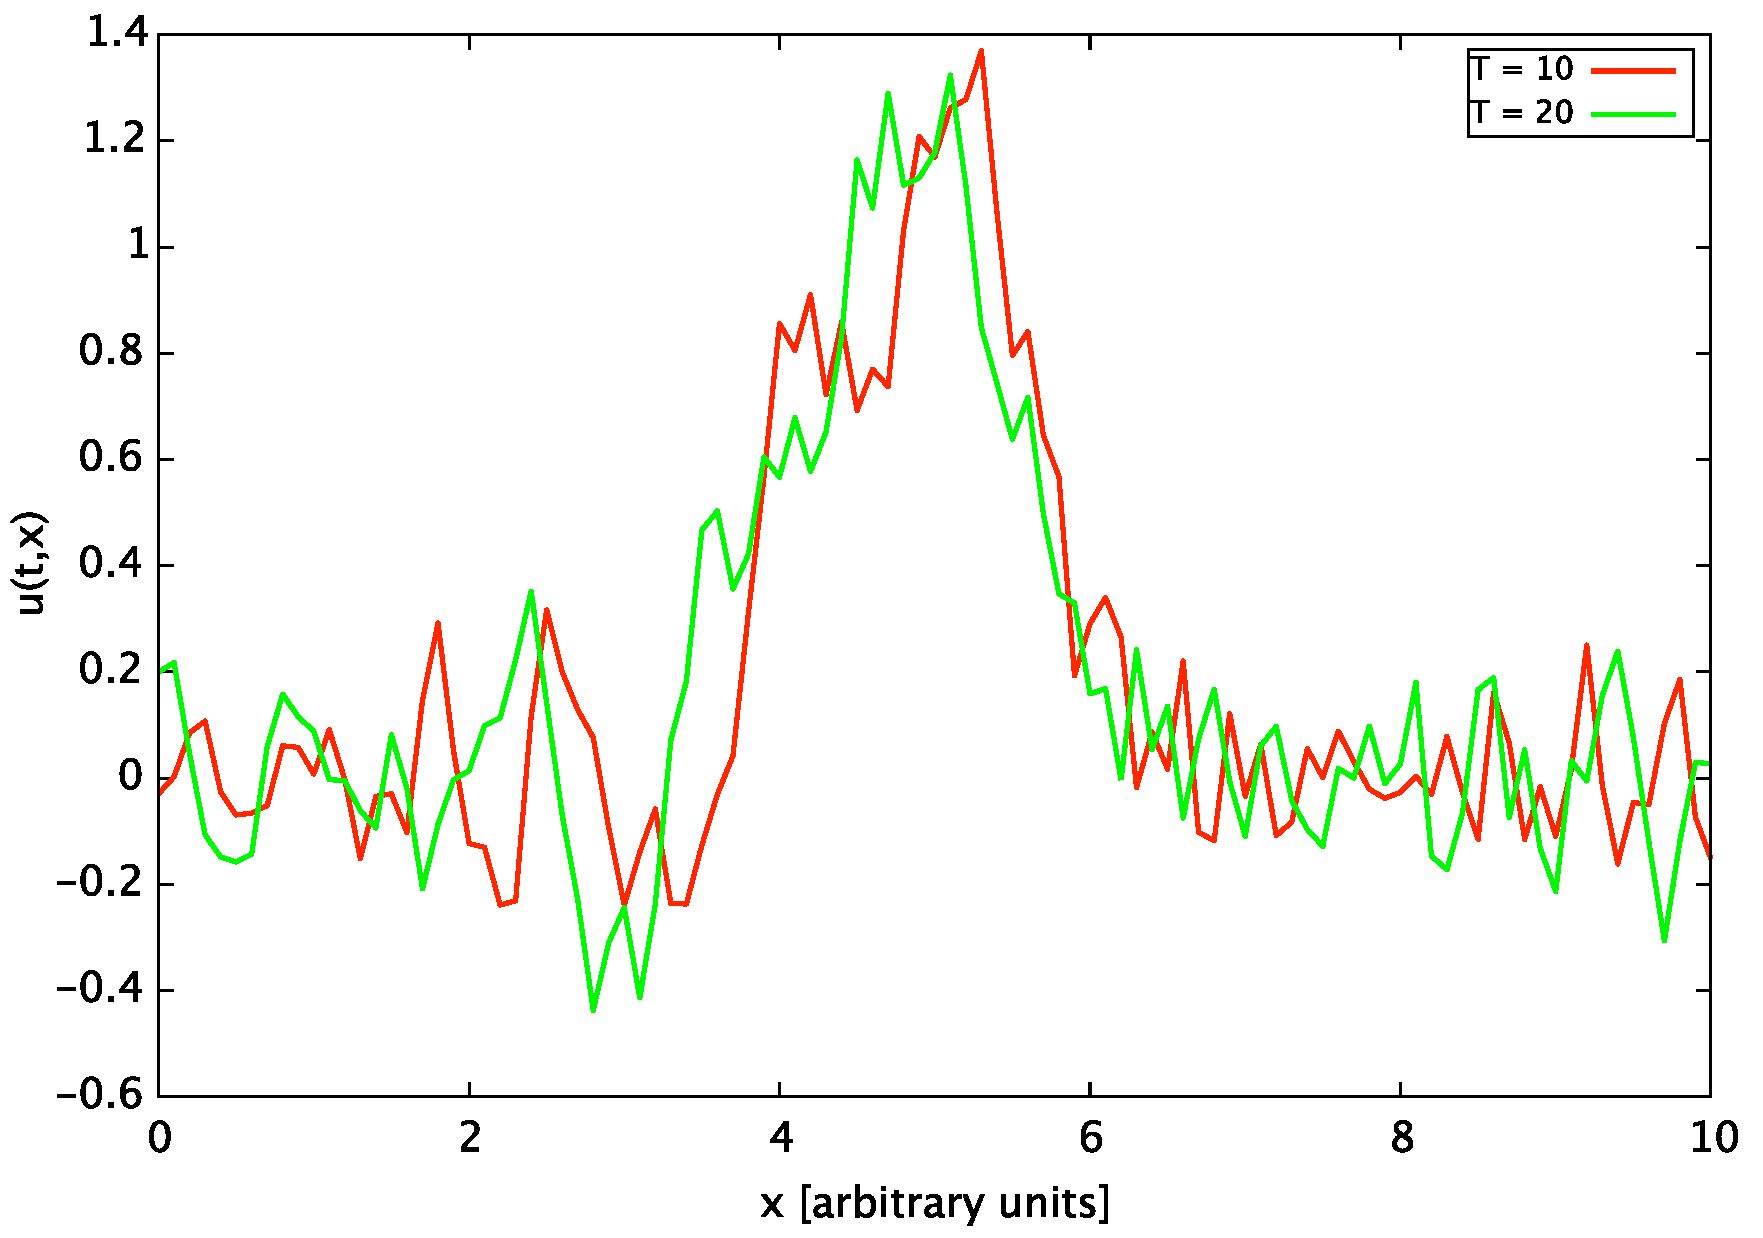
\includegraphics[scale=0.25]{good_img/lf_nuovo1}}
\subfigure[$u(x,t=10)$ with $c_f=0.5$ and $\Delta x = 0.01$]
{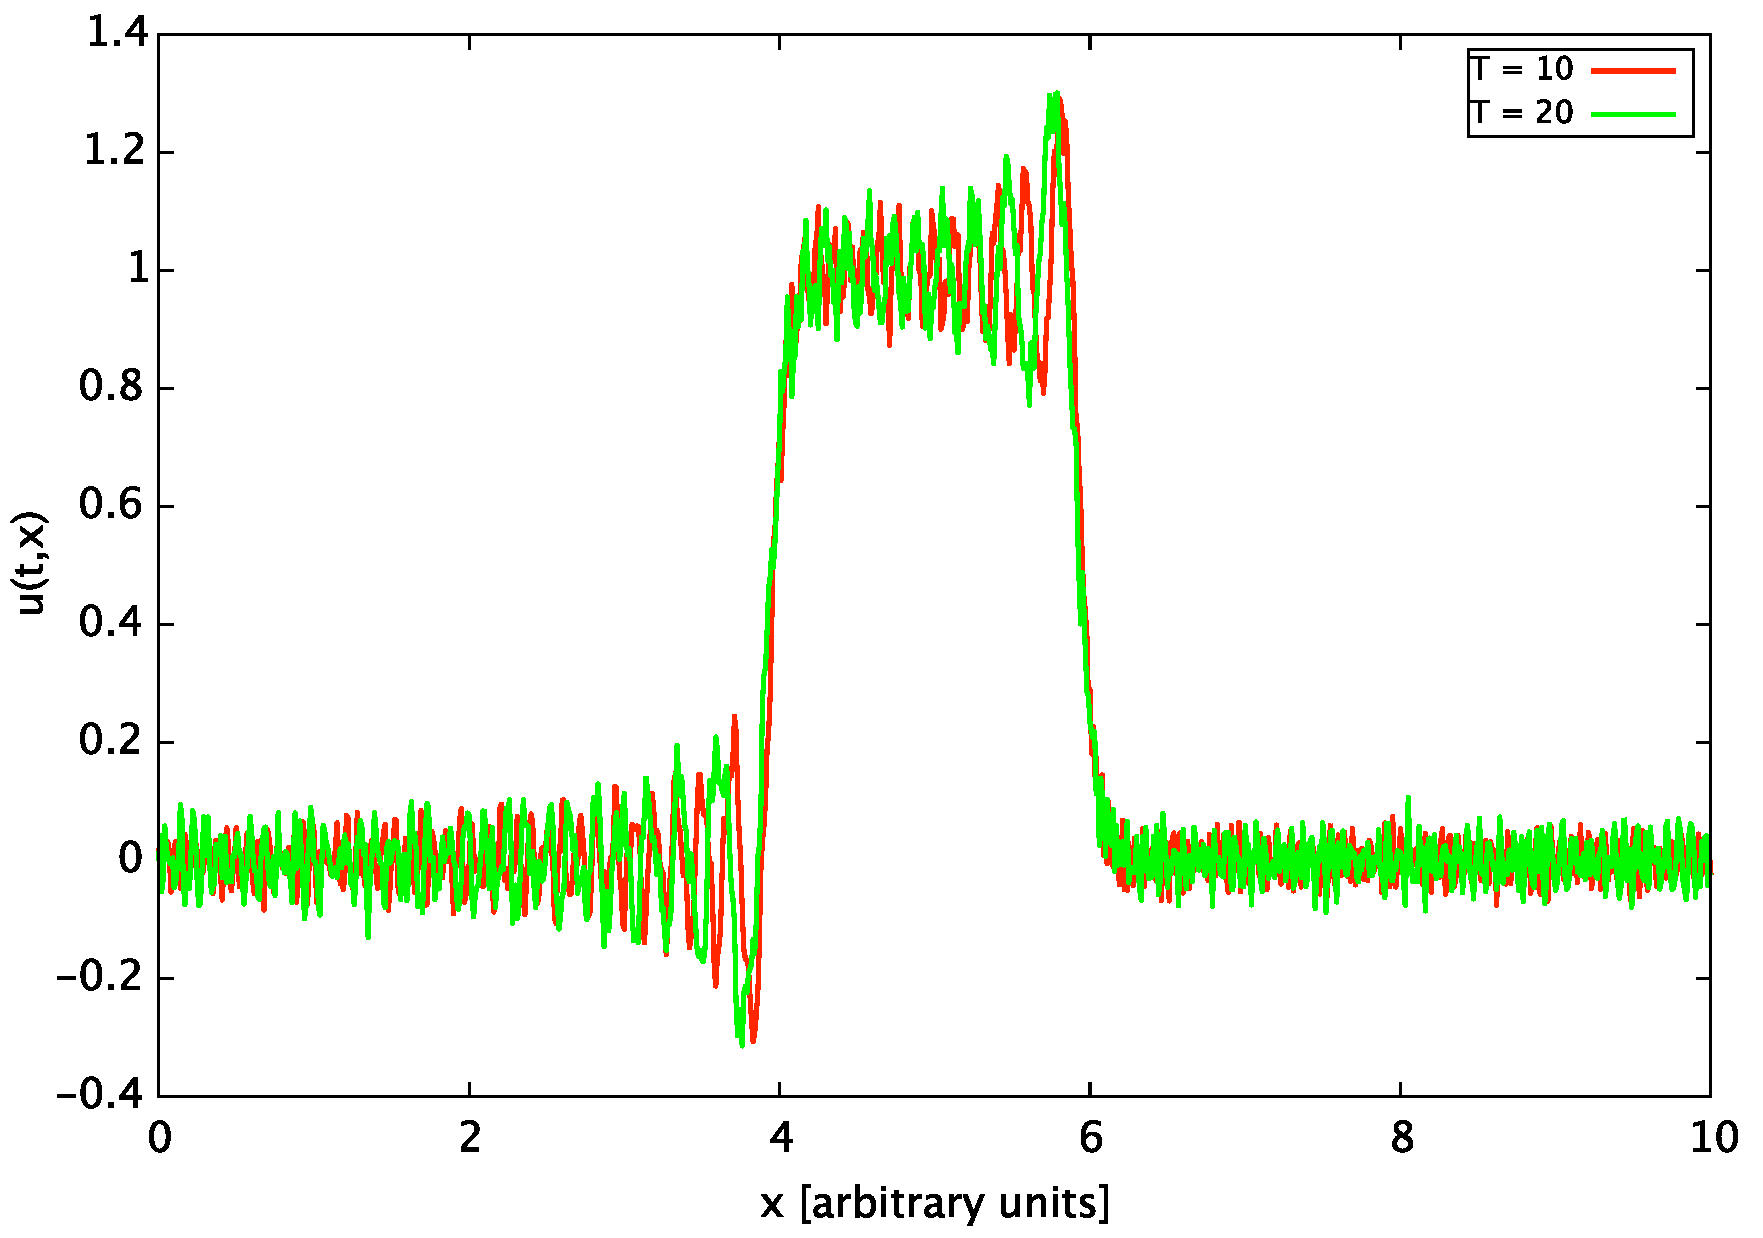
\includegraphics[scale=0.25]{good_img/lf_cf05_dx001_s}}
\end{figure}
It is clear that leapfrog is not a good method to integrate advection equation in case of square wave initial condition. The problem lies in the fact that the algorithm is not monotonous, and produces oscillations when discontinuities are encoutered. However, with $c_f=1$ the problem is solved correctly (Fig. 1.15, 1.16).
\begin{figure}[!h]
\centering
\subfigure[$u(x,t=10)$ with $c_f=1$]
{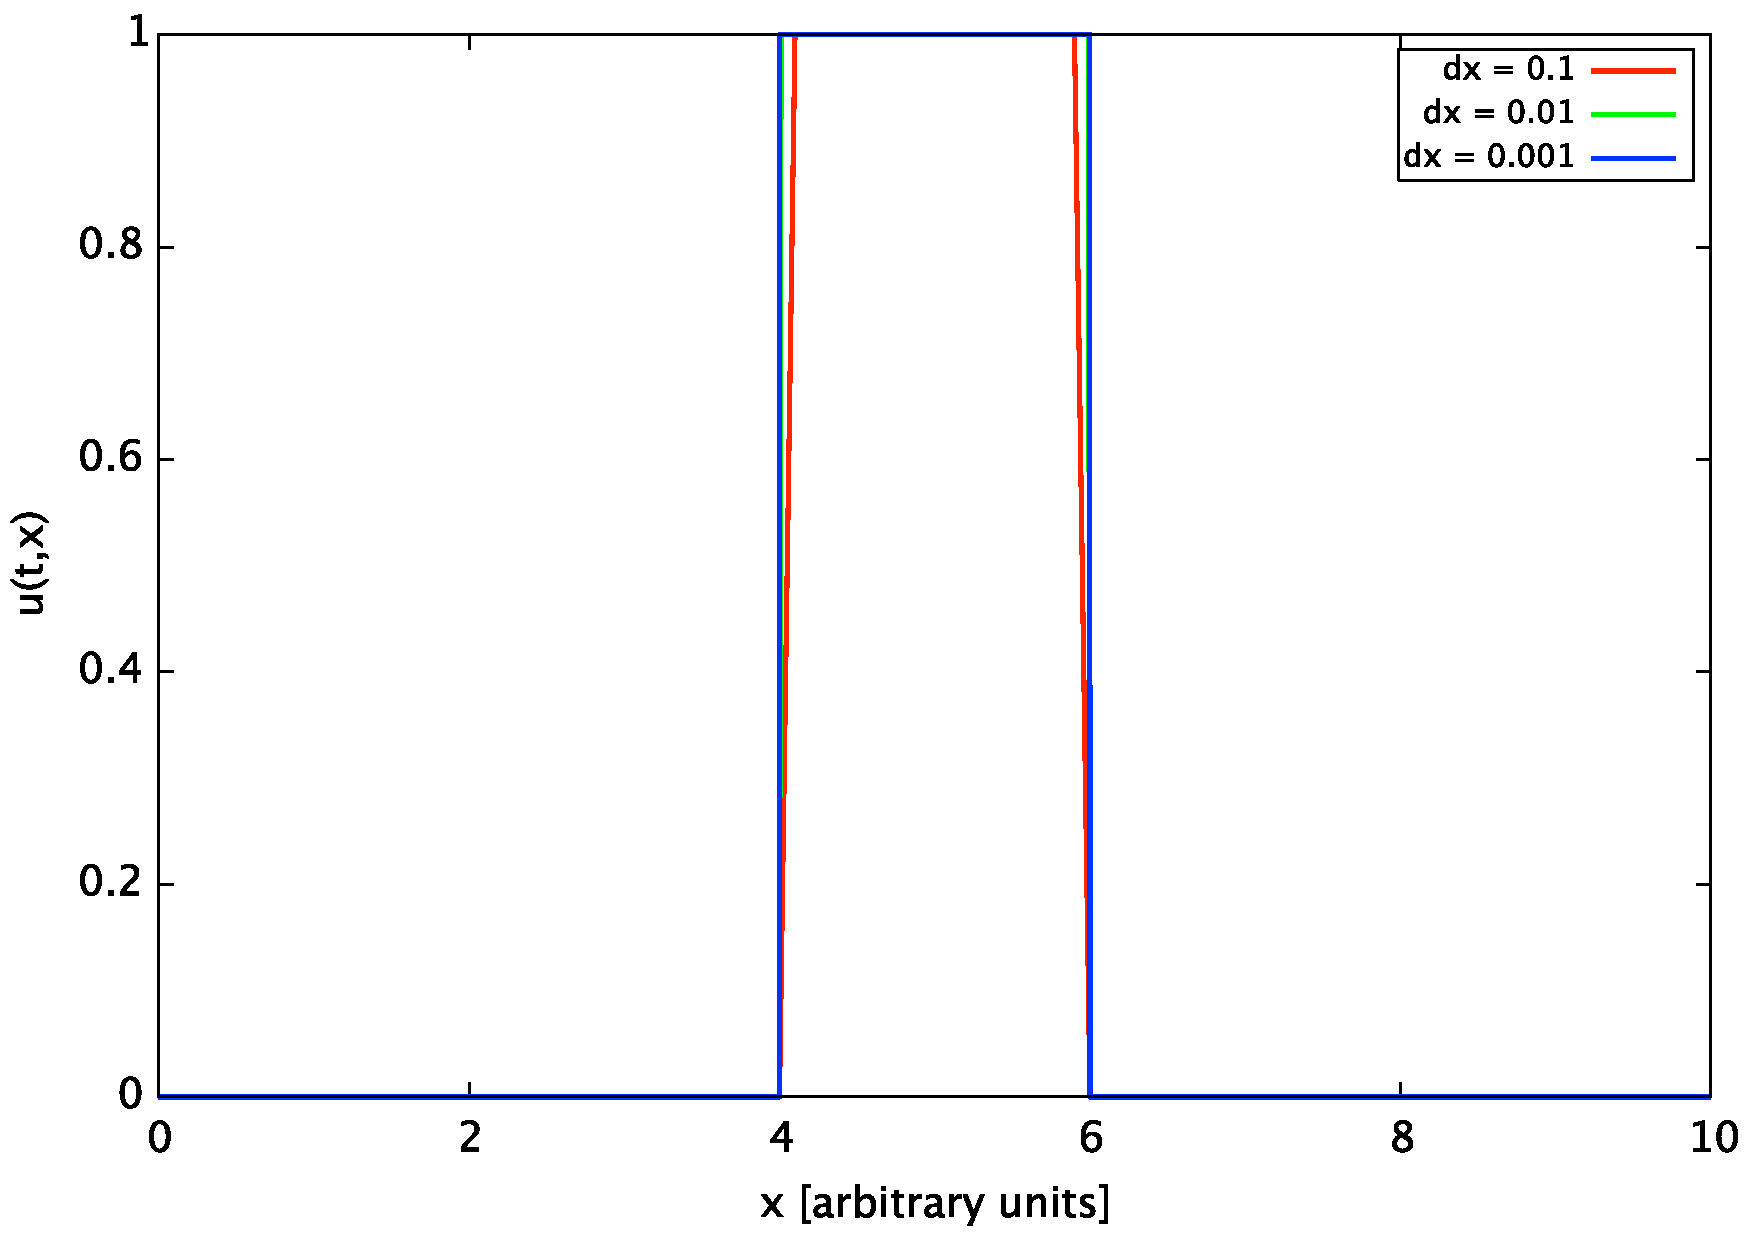
\includegraphics[scale=0.25]{good_img/fig115}}
\subfigure[$u(x,t=20)$ with $c_f=1$]
{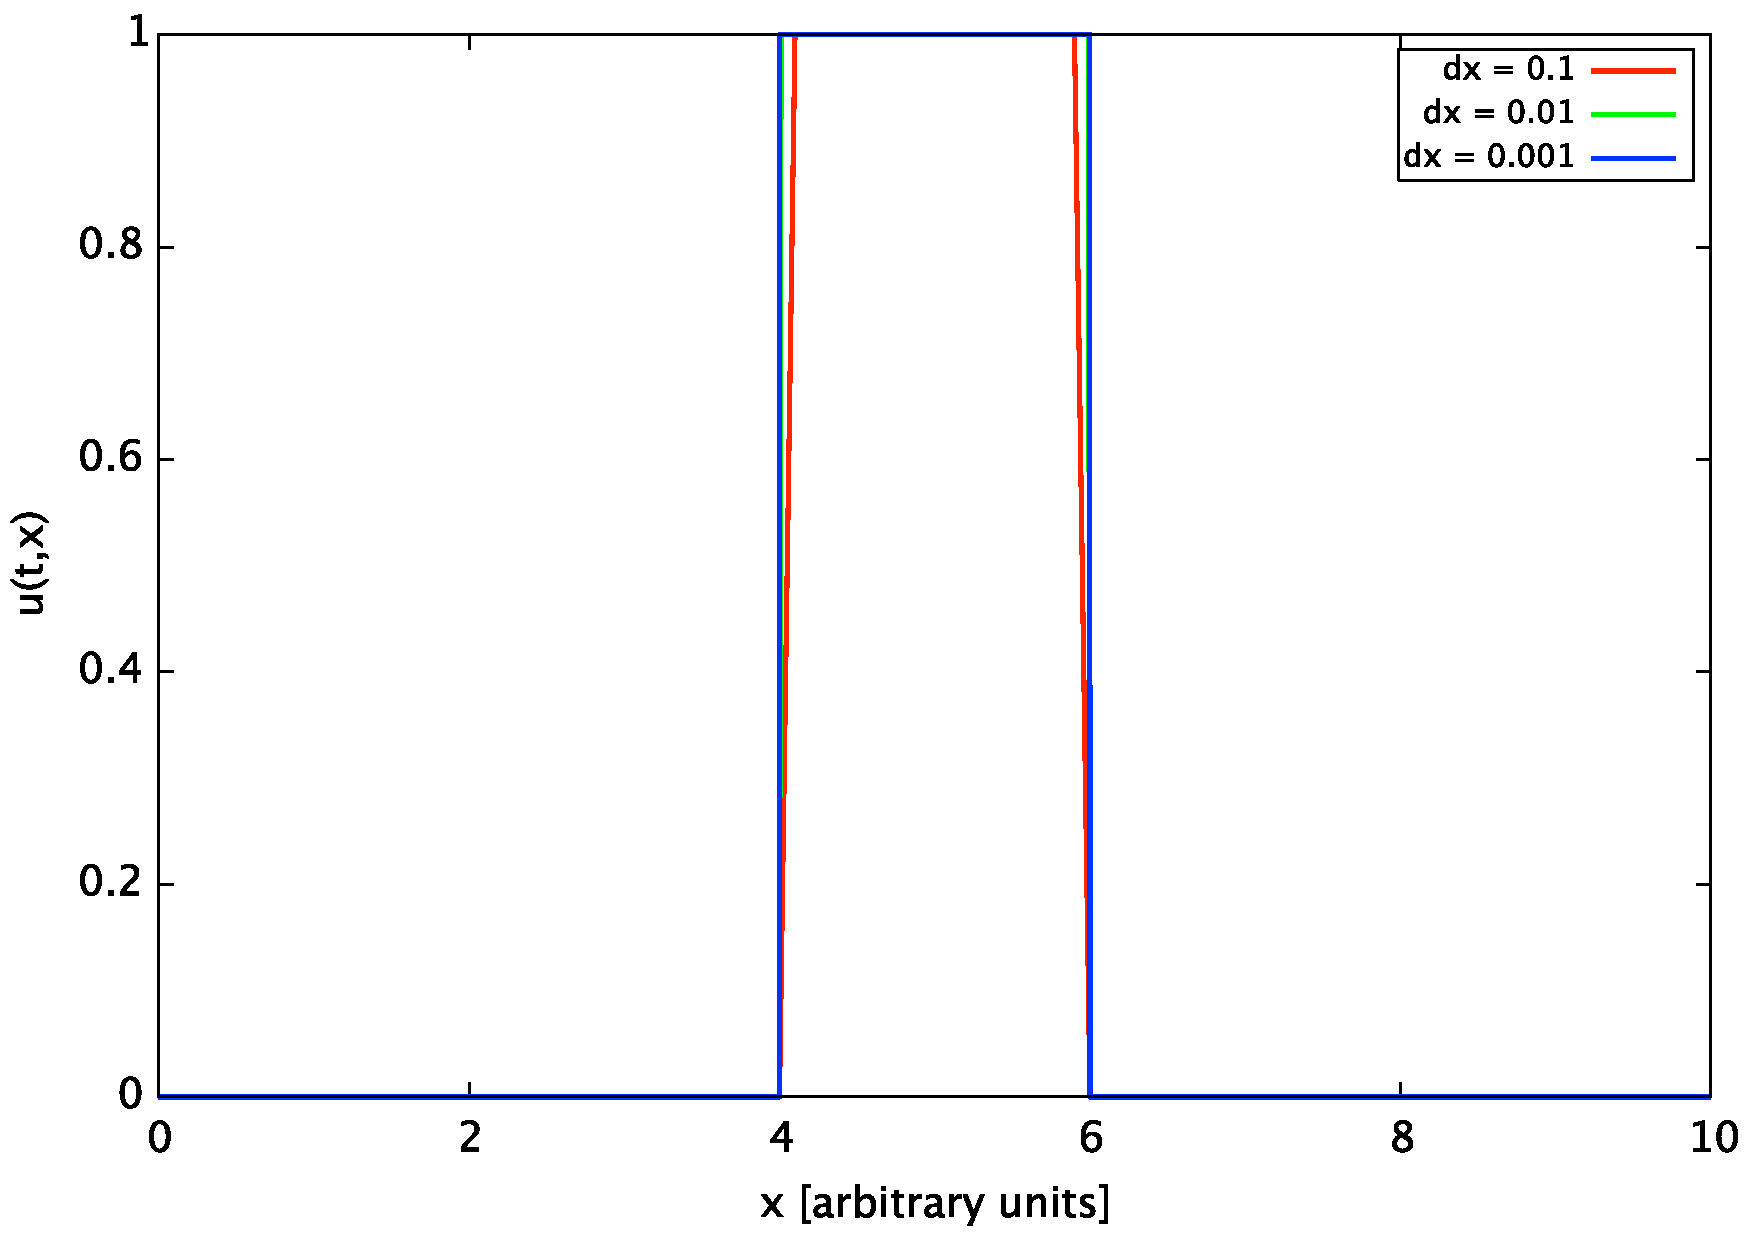
\includegraphics[scale=0.25]{good_img/leap_nuovo2}}
\end{figure}
Therefore, the Leapfrog algorithm with $\Delta x \leq 0.01$ and gaussian initial condition is a reliable method to solve the advection equation, while with square wave initial condition with $c_f = 0.5$ it is not. The L2-norms for both the gaussian and square wave initial conditions in the case of $c_f=0.5$ follow (Fig. 1.17, 1.18). 
\begin{figure}[!h]
\centering
\subfigure[L2-norm with $c_f=0.5$ and $\Delta x = 0.1$ for the Gaussian initial condition]
{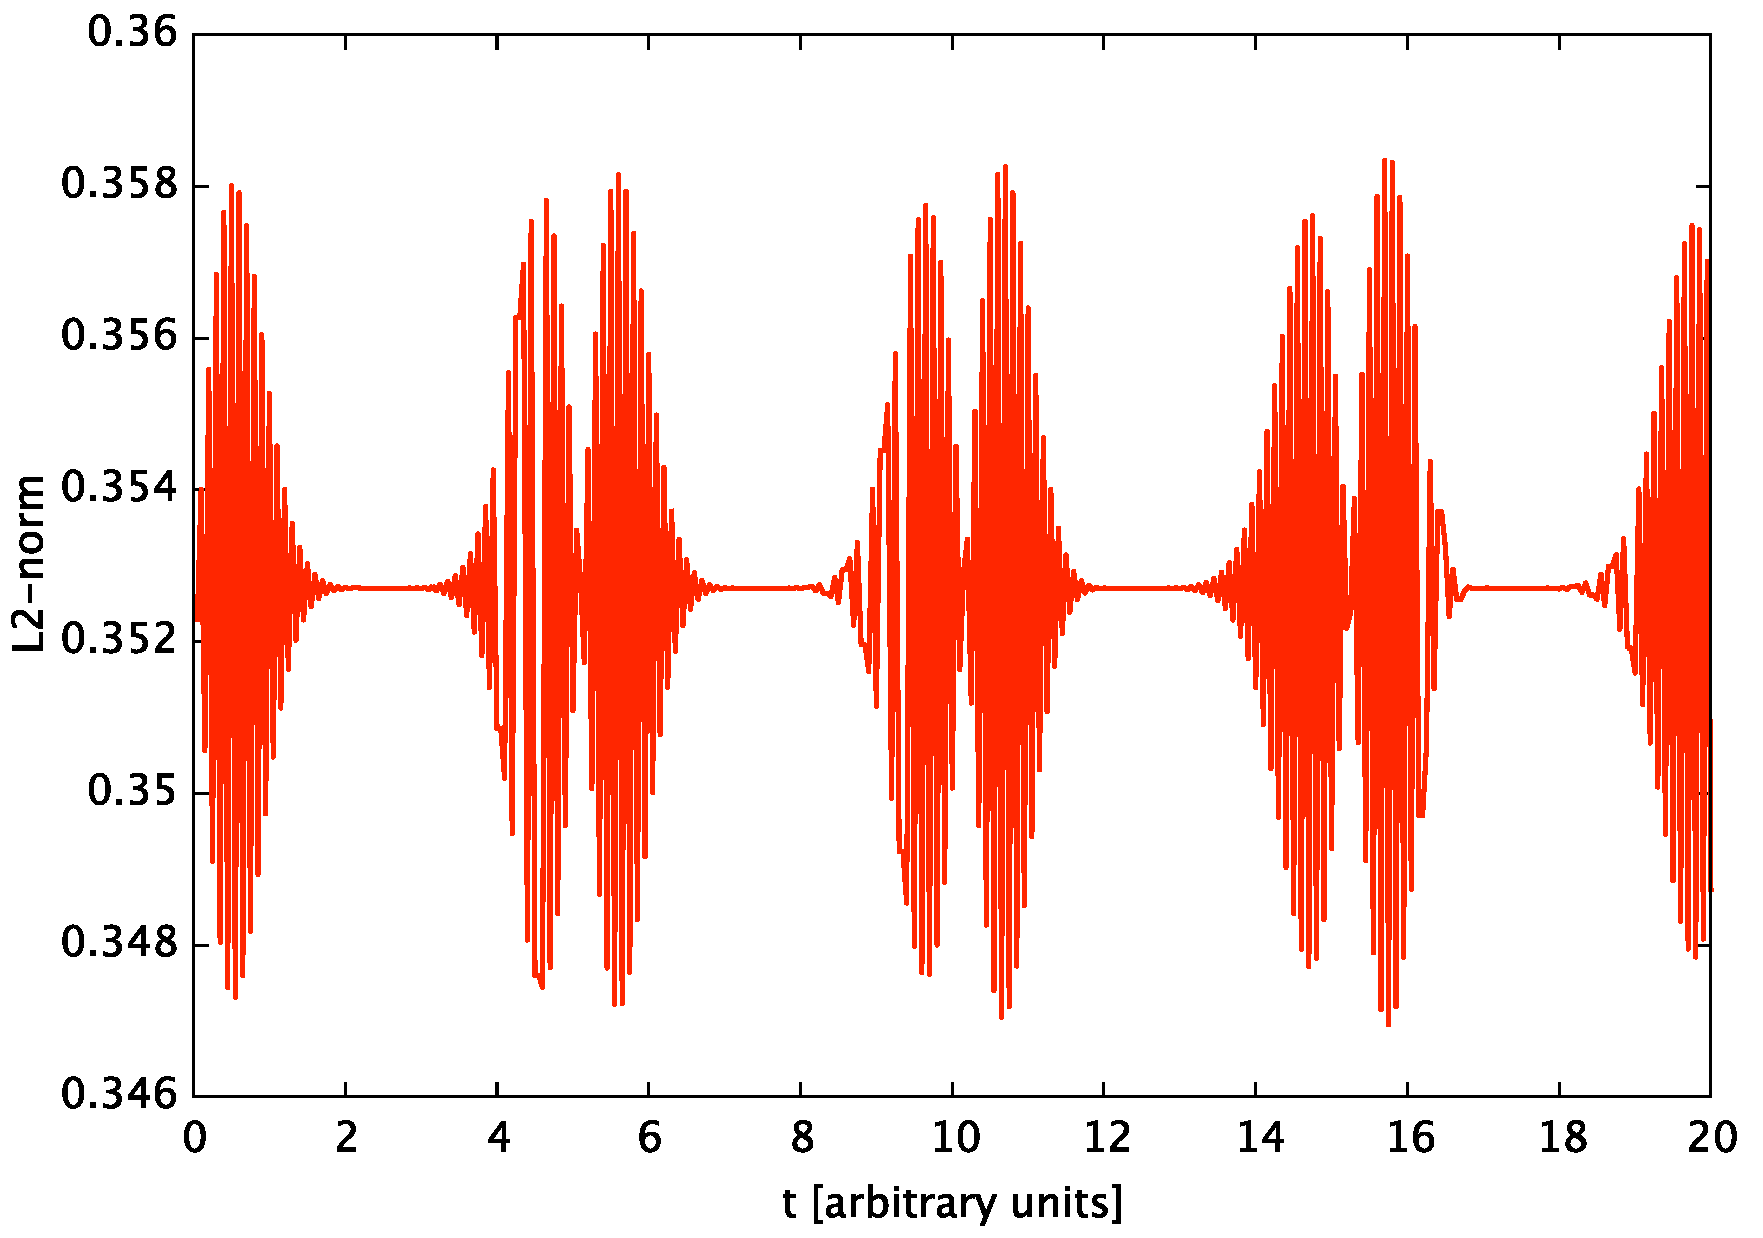
\includegraphics[scale=0.25]{good_img/lefr_l2_g}}
\subfigure[L2-norm with $c_f=0.5$ and $\Delta x = 0.1$ for the square wave initial condition]
{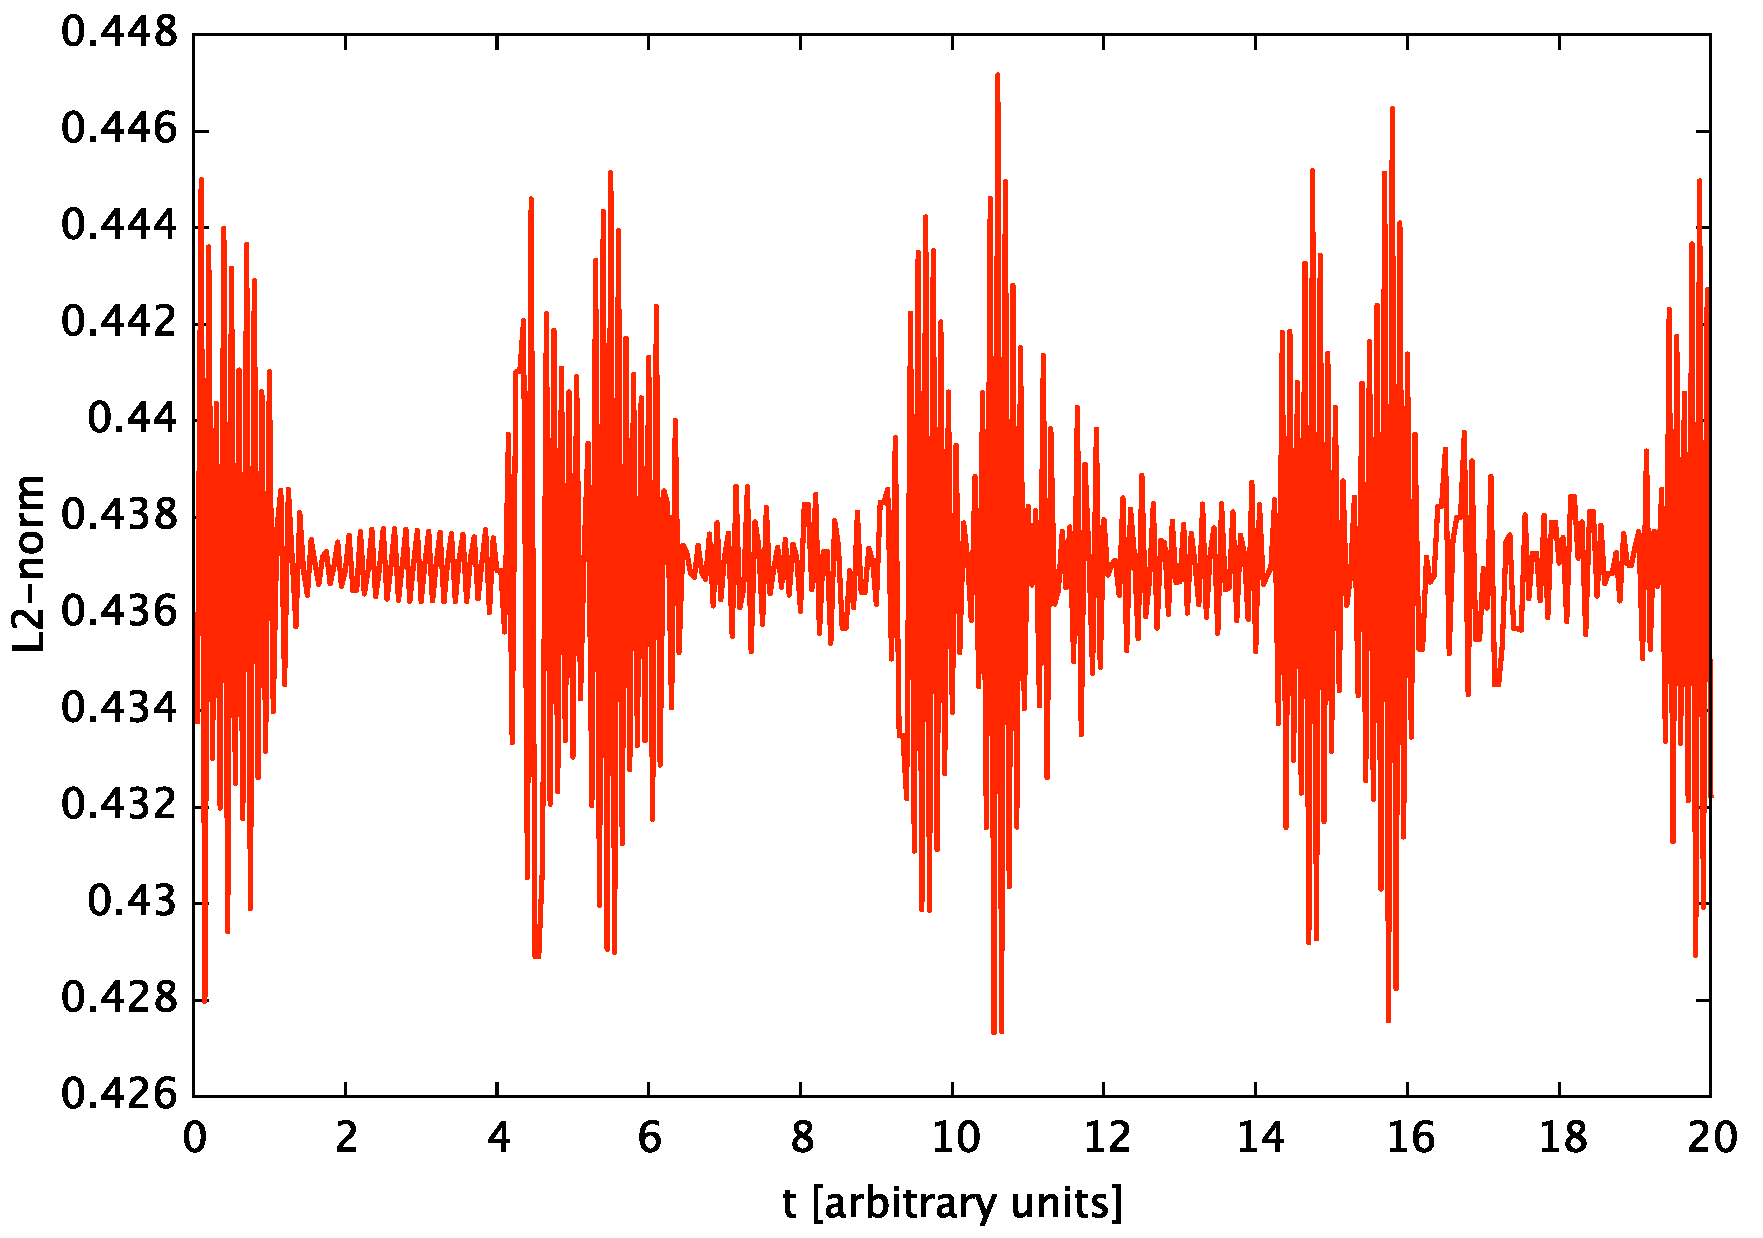
\includegraphics[scale=0.25]{good_img/lefr_l2_s}}
\end{figure}
\section{The Lax-Friedrichs method}
The \emph{Lax-Friedrichs method} is a stable method (under the condition $|a|\frac{\Delta t}{\Delta x} \leq 1$) to solve the advection equation described by the following algorithm:
\begin{equation}
u_j^{n+1} = \frac{1}{2} (u_{j-1}^n + u_{j+1}^n) - a\frac{\Delta t}{2\Delta x}(u_{j+1}^n - u_{j-1}^n)
\end{equation}
\begin{figure}[!h]
\centering
\subfigure[$u(x,t=10)$ with $c_f=0.5$]
{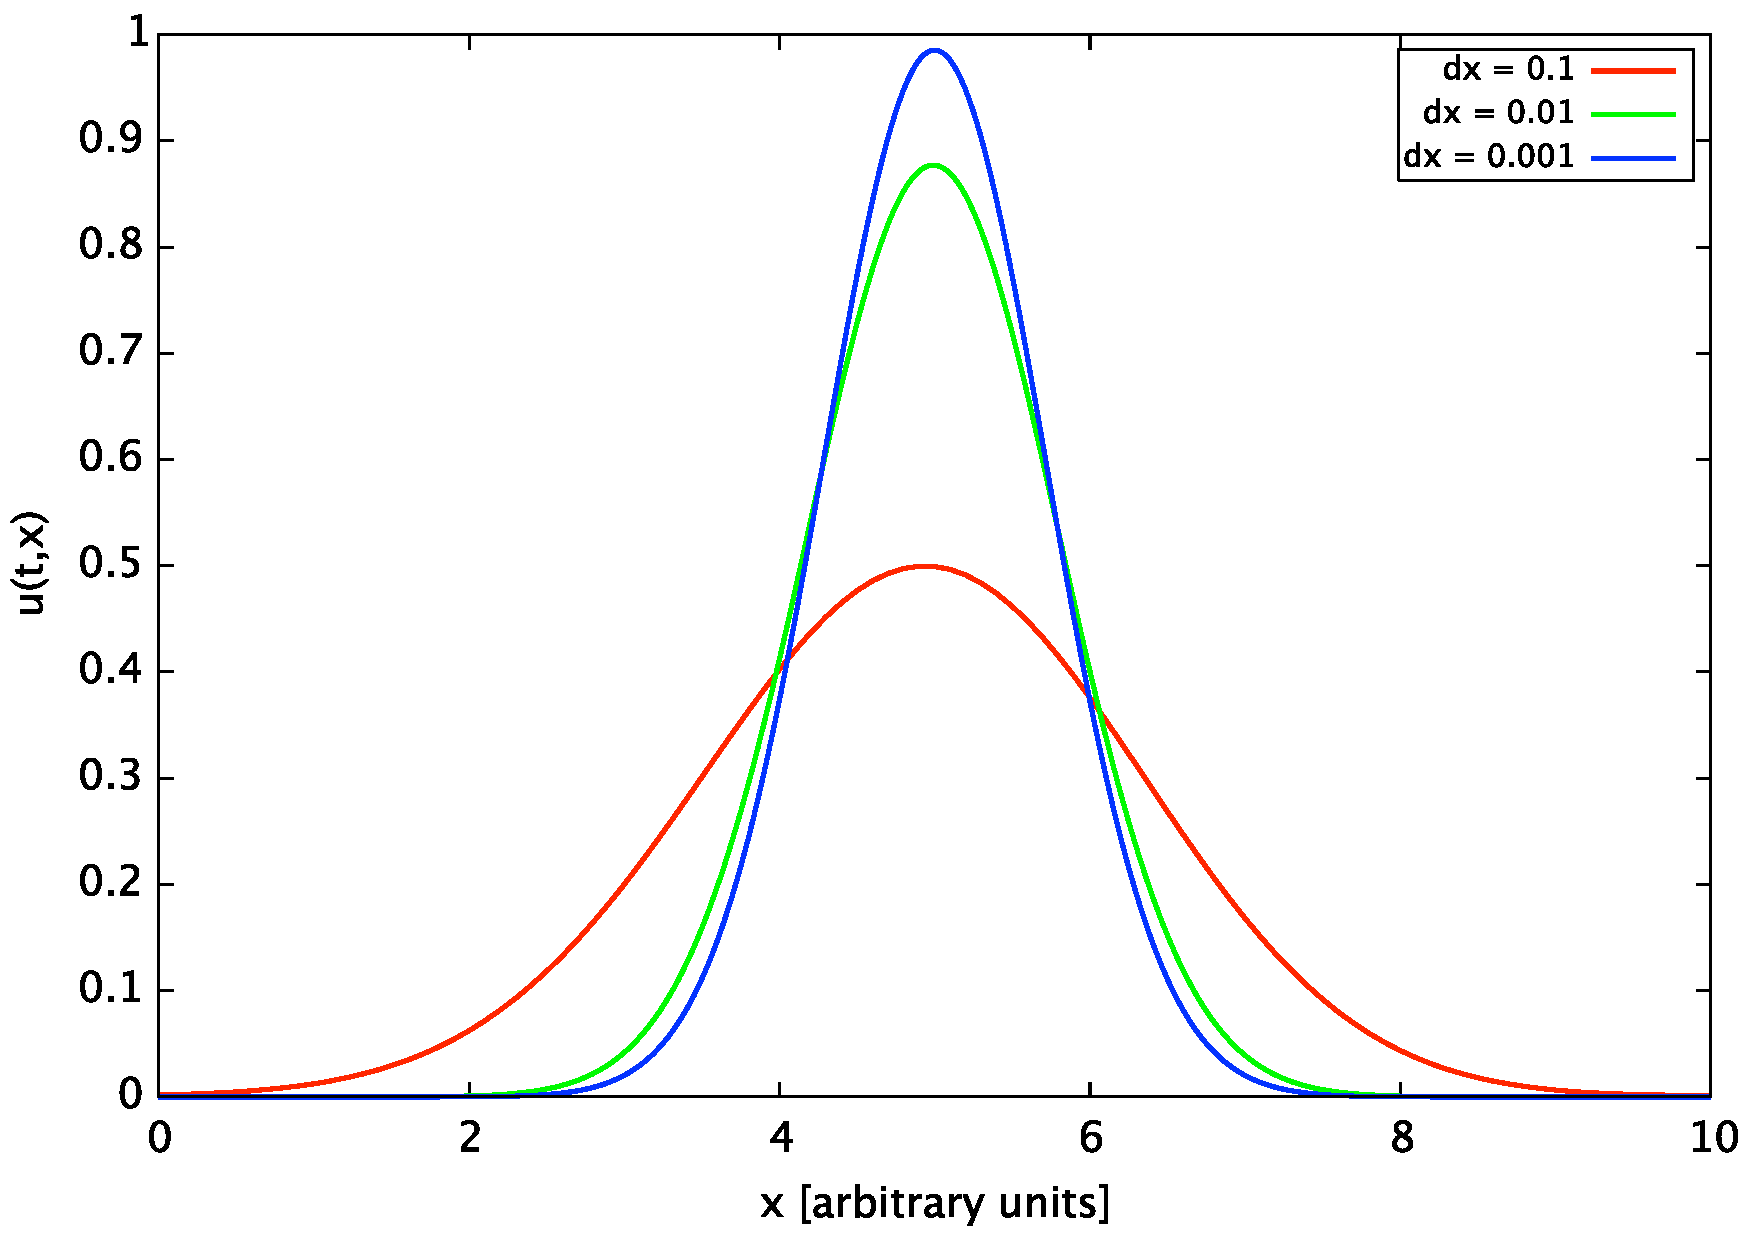
\includegraphics[scale=0.25]{good_img/lxfr_cf05_t10_g}}
\subfigure[$u(x,t=20)$ with $c_f=0.5$]
{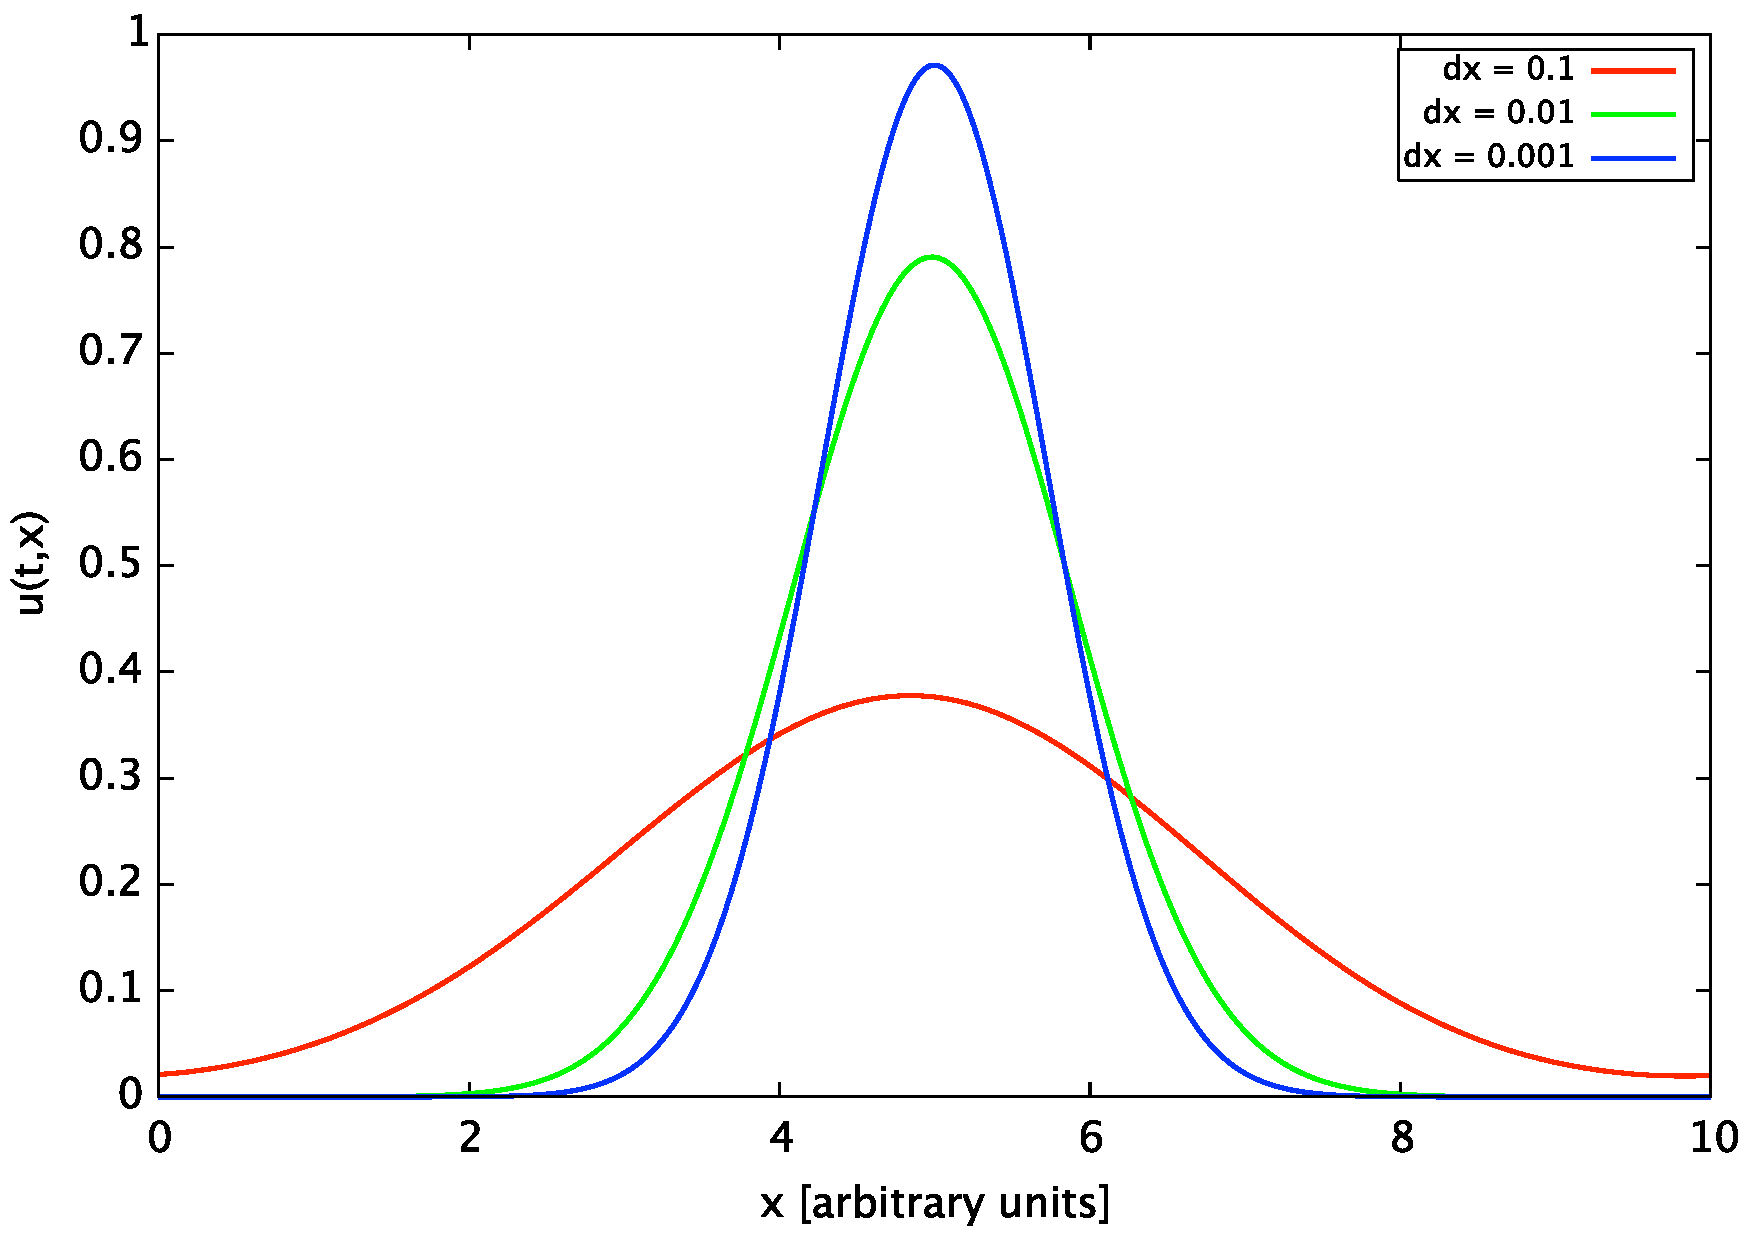
\includegraphics[scale=0.25]{good_img/lxfr_cf05_t20_g}}
\subfigure[$u(x,t=10)$ with $c_f=1$]
{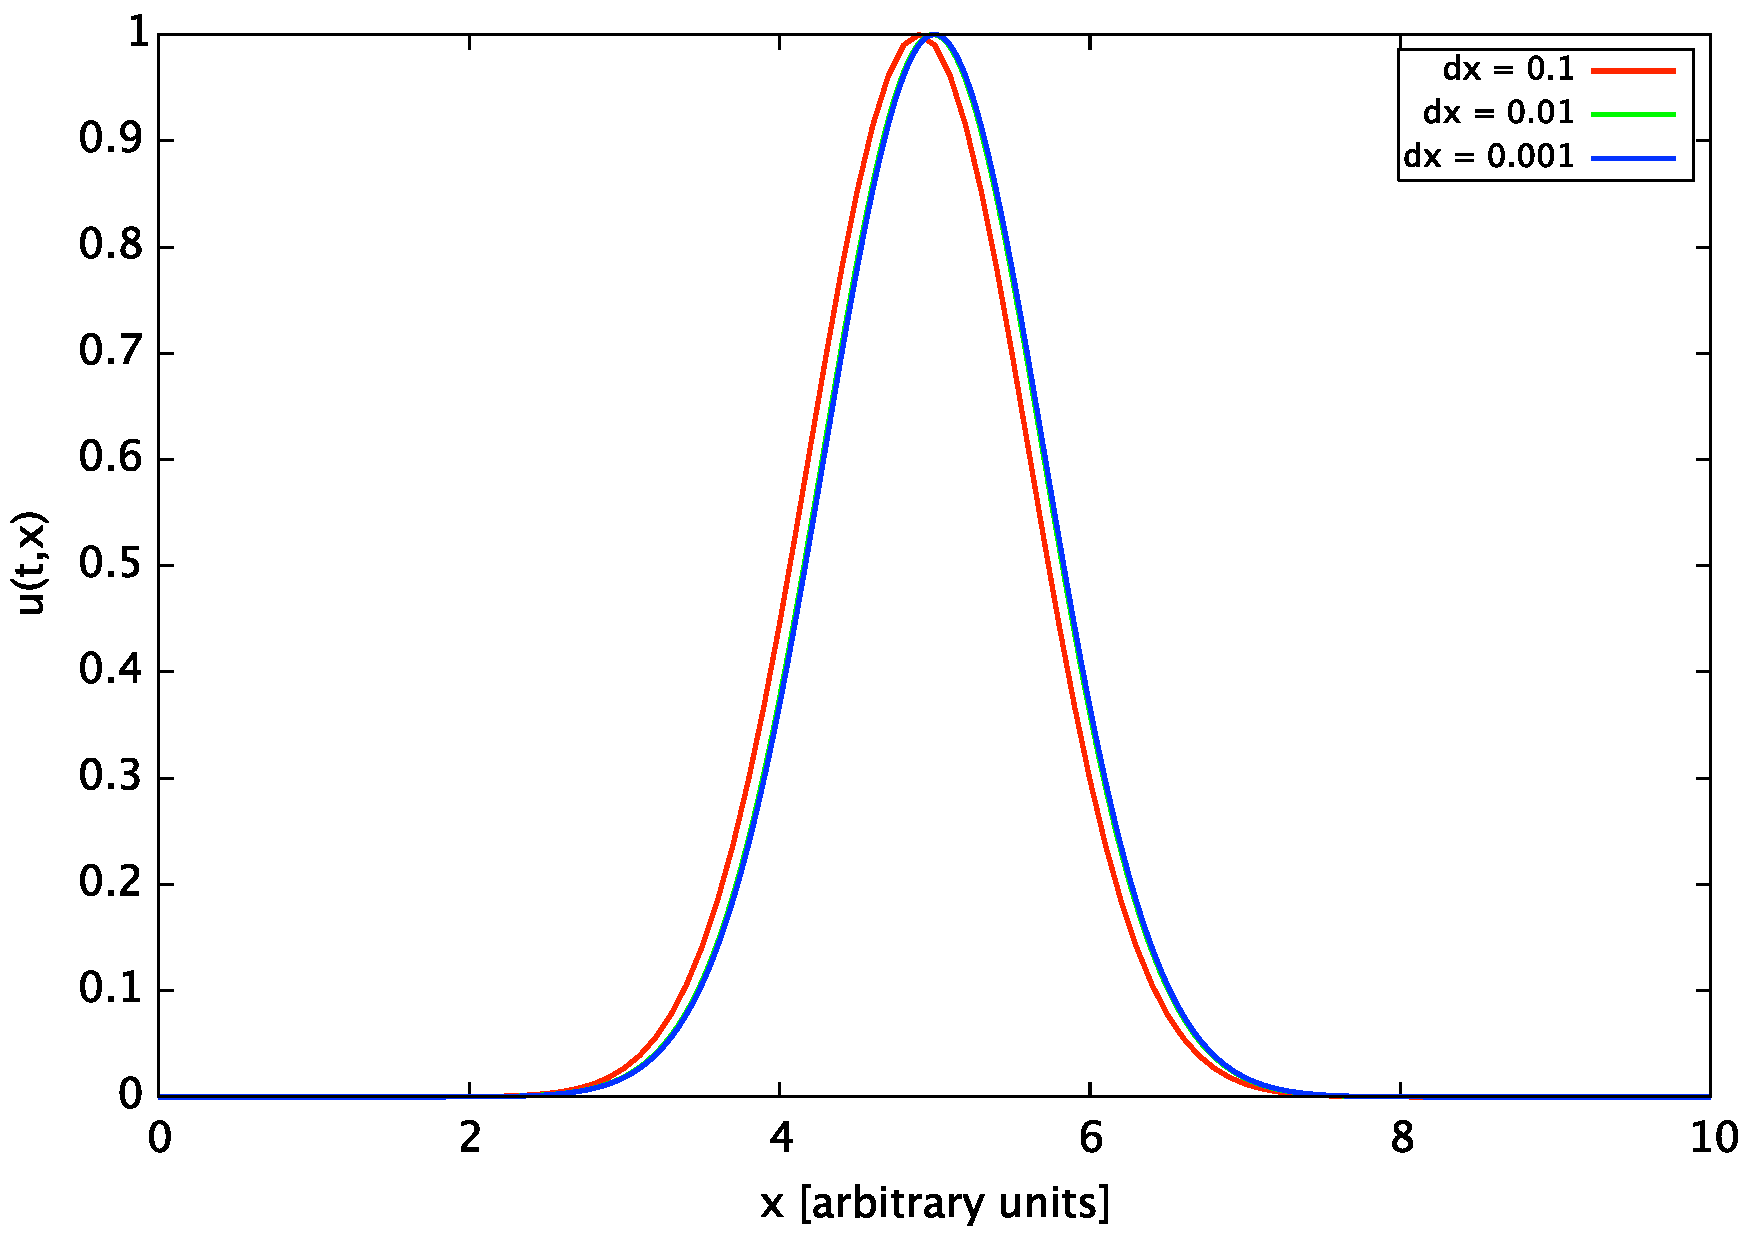
\includegraphics[scale=0.25]{good_img/lxfr_cf1_t10_g}}
\subfigure[$u(x,t=20)$ with $c_f=1$]
{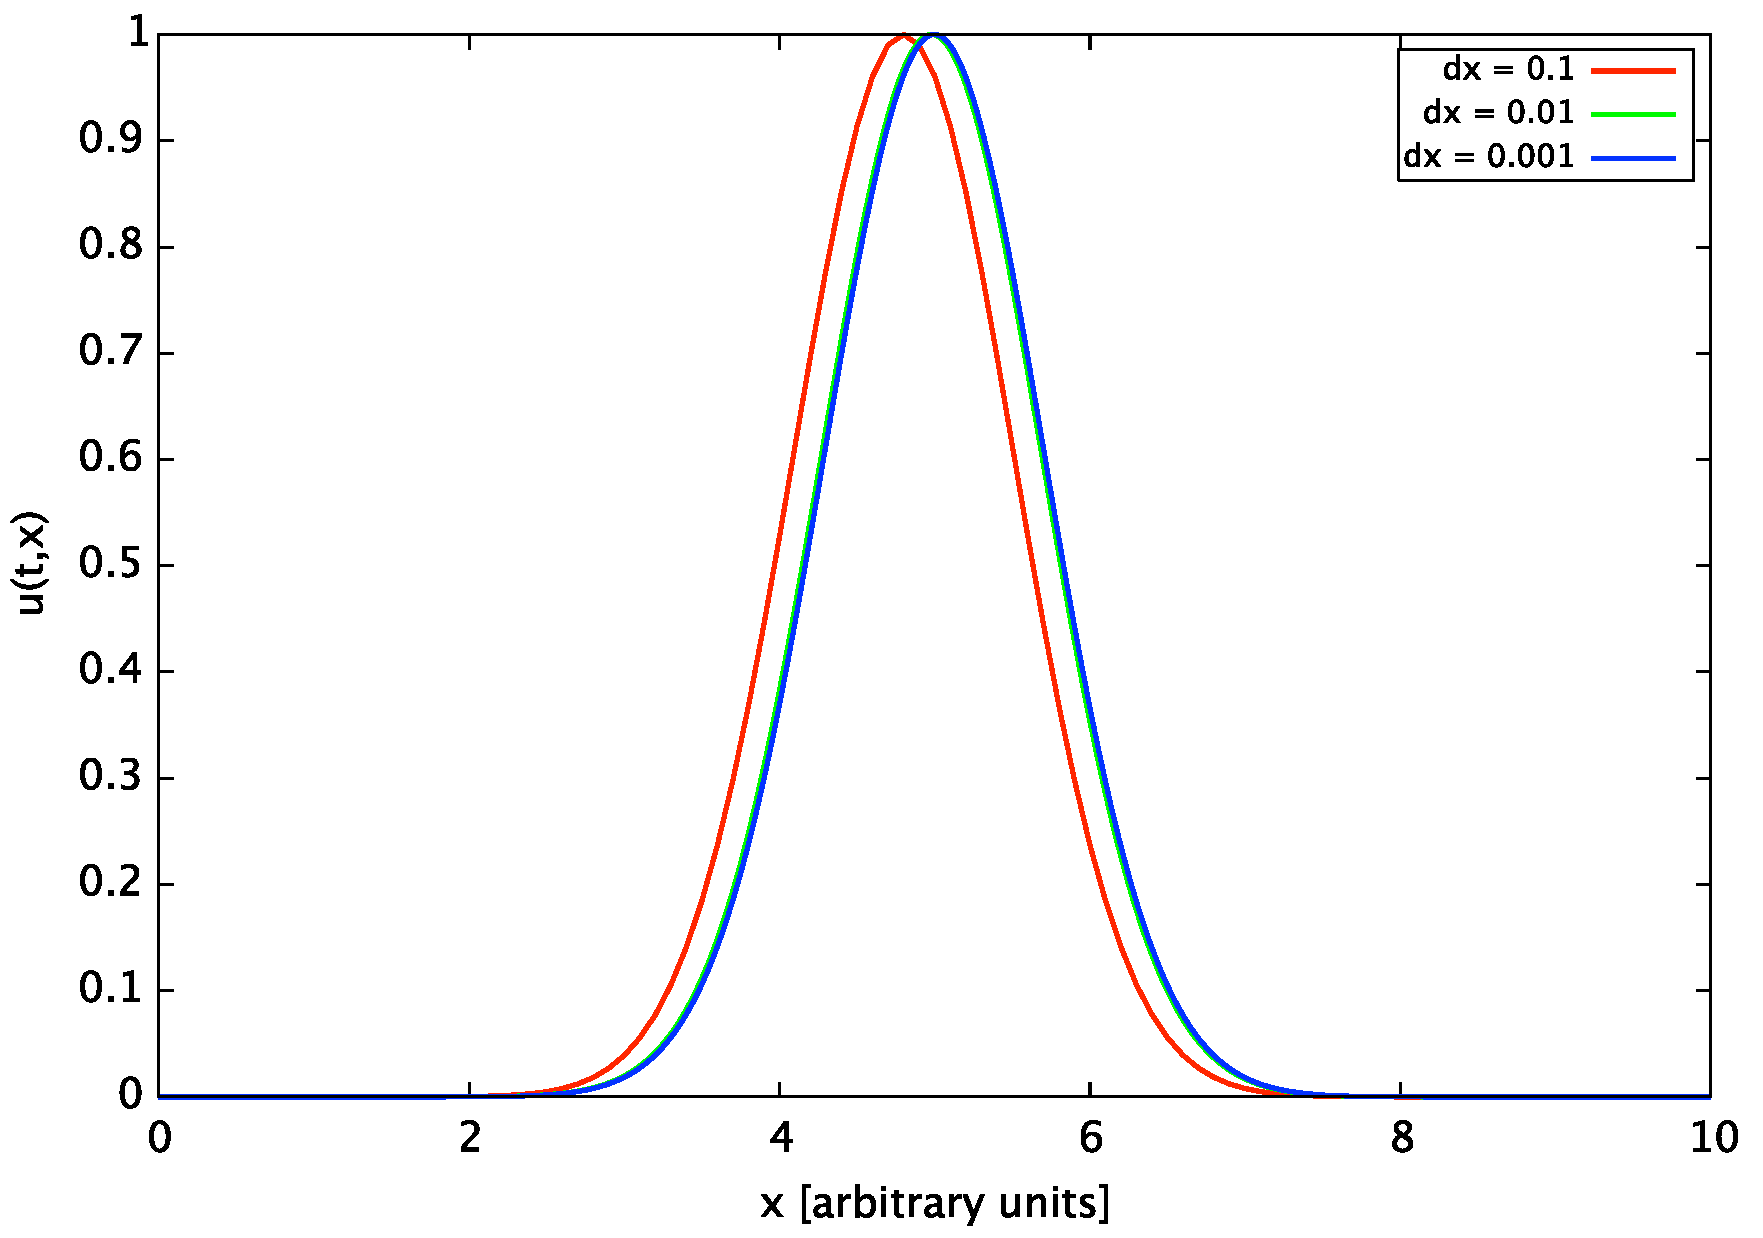
\includegraphics[scale=0.25]{good_img/lxfr_cf1_t20_g}}
\end{figure}\\
where the first factor on the right-hand side of (9) is obtained by substituting $u_j^n$ with its mean value. Let's look at some results obtained implementing the algorithm for initial condition (1) with different parameters (Fig. 1.19 - 1.22). The fact that with $c_f=0.5$ we have an evident dissipation effect is easily explained by observing that the substitution $u_j^n \to \frac{1}{2} (u_{j-1}^n + u_{j+1}^n)$ introduces a dissipative term in the starting differential equation:
\begin{equation}
\frac{\partial t}{\partial t} + a \frac{\partial u}{\partial x} = \frac{1}{2} \frac{\Delta x^2}{\Delta t} \frac{\partial^2 u}{\partial x^2} + o(\Delta x^2)
\end{equation}
where
\begin{equation}
\frac{\Delta x^2}{\Delta t} = \frac{\Delta x^2}{c_f\frac{\Delta x}{|a|}} \propto \Delta x
\end{equation}
Therefore the dissipative effect is proportional to the mesh spacing, as clearly stressed by the simulations. With $c_f = 1$ the situation is different because the Lax-Friedrichs algorithm reduces to
\[
u_j^{n+1} = \frac{1}{2}(\slashed{u_{j+1}^n} + u^n_{j-1}) - \frac{1}{2}(\slashed{u^n_{j+1}} - u_{j-1}^n) = u^n_{j-1}
\] 
that means
\begin{equation}
u_j^{n+1} = u^n_{j-1}
\end{equation}
which is indeed the analytic solution of the advection equation in case of $a = c_f = 1$. Let's look at the results obtained with initial condition (2) (Fig. 1.23 - 1.26). 
\begin{figure}[!h]
\centering
\subfigure[$u(x,t=10)$ with $c_f=0.5$]
{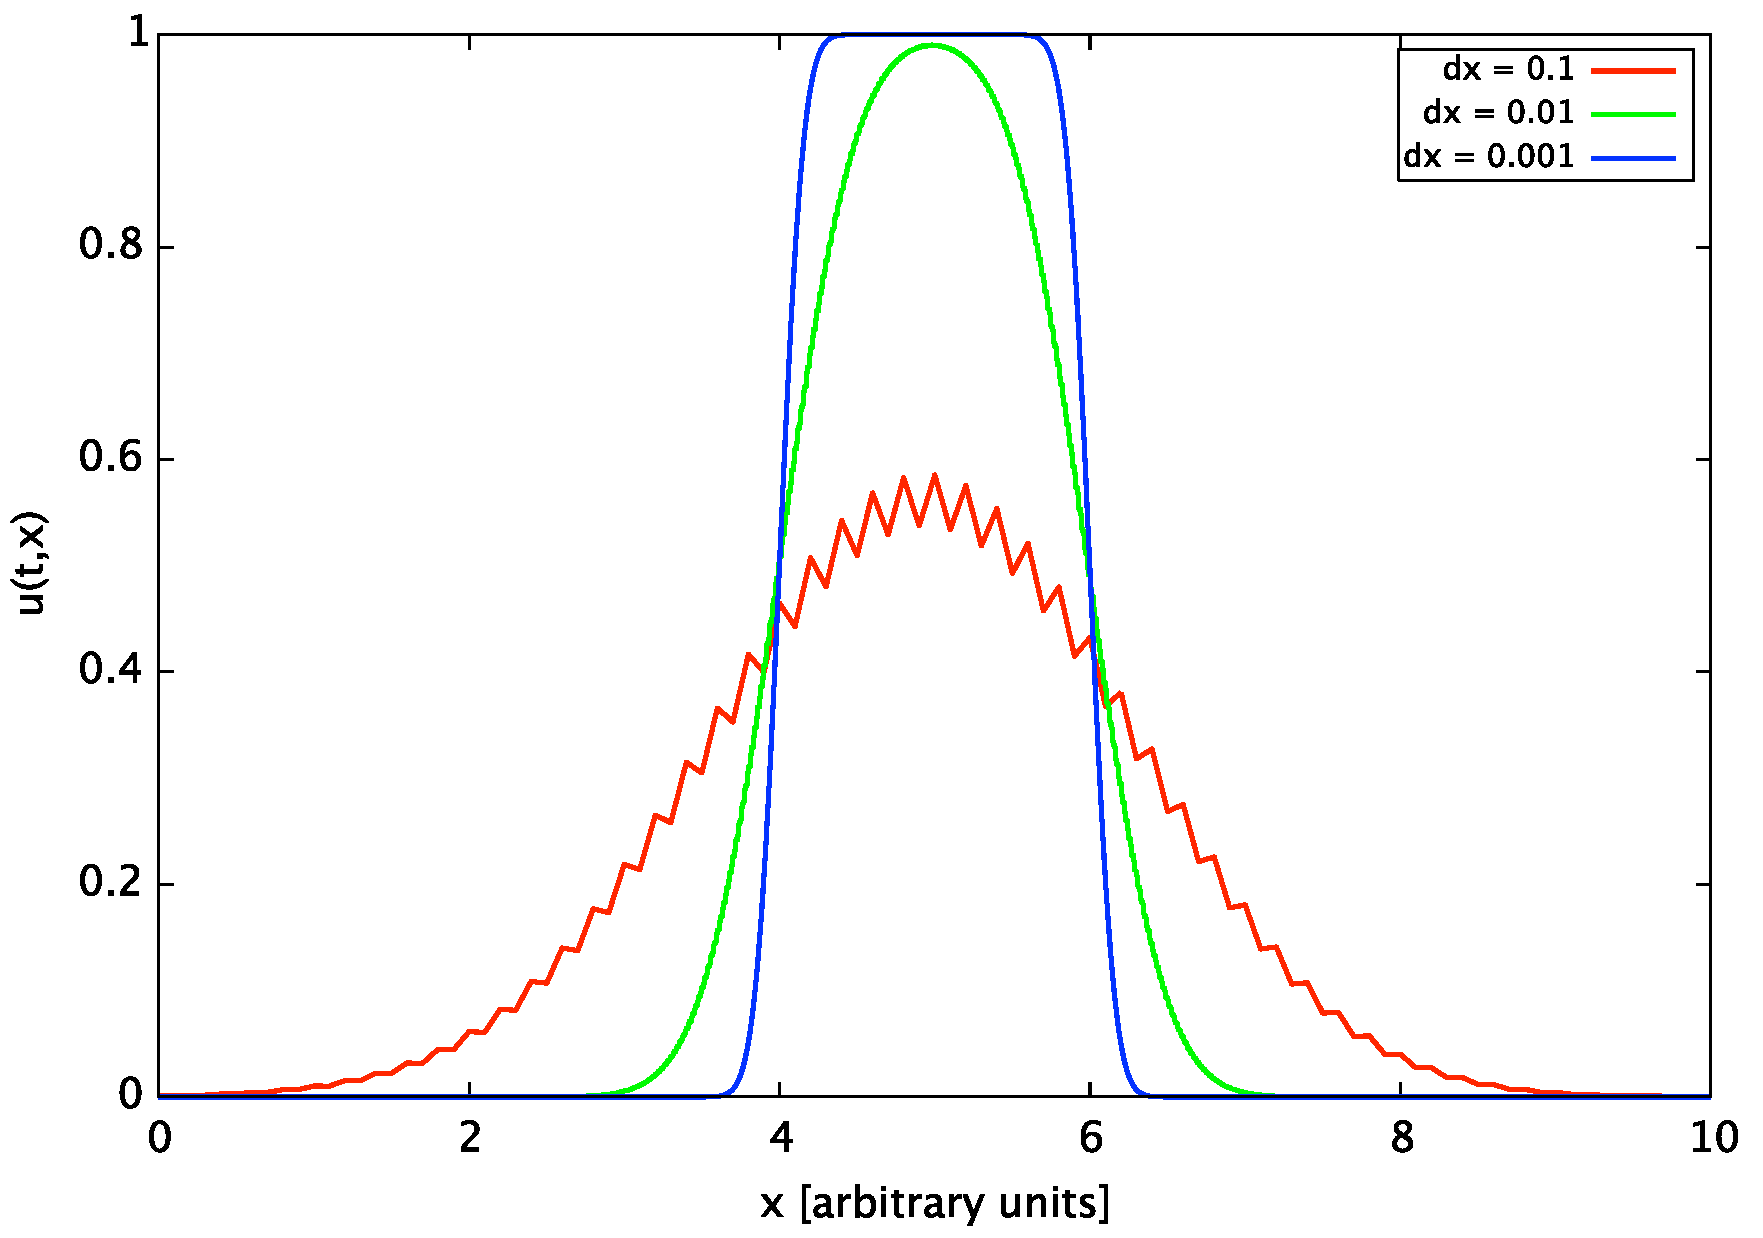
\includegraphics[scale=0.25]{good_img/lxfr_cf05_t10_s}}
\subfigure[$u(x,t=20)$ with $c_f=0.5$]
{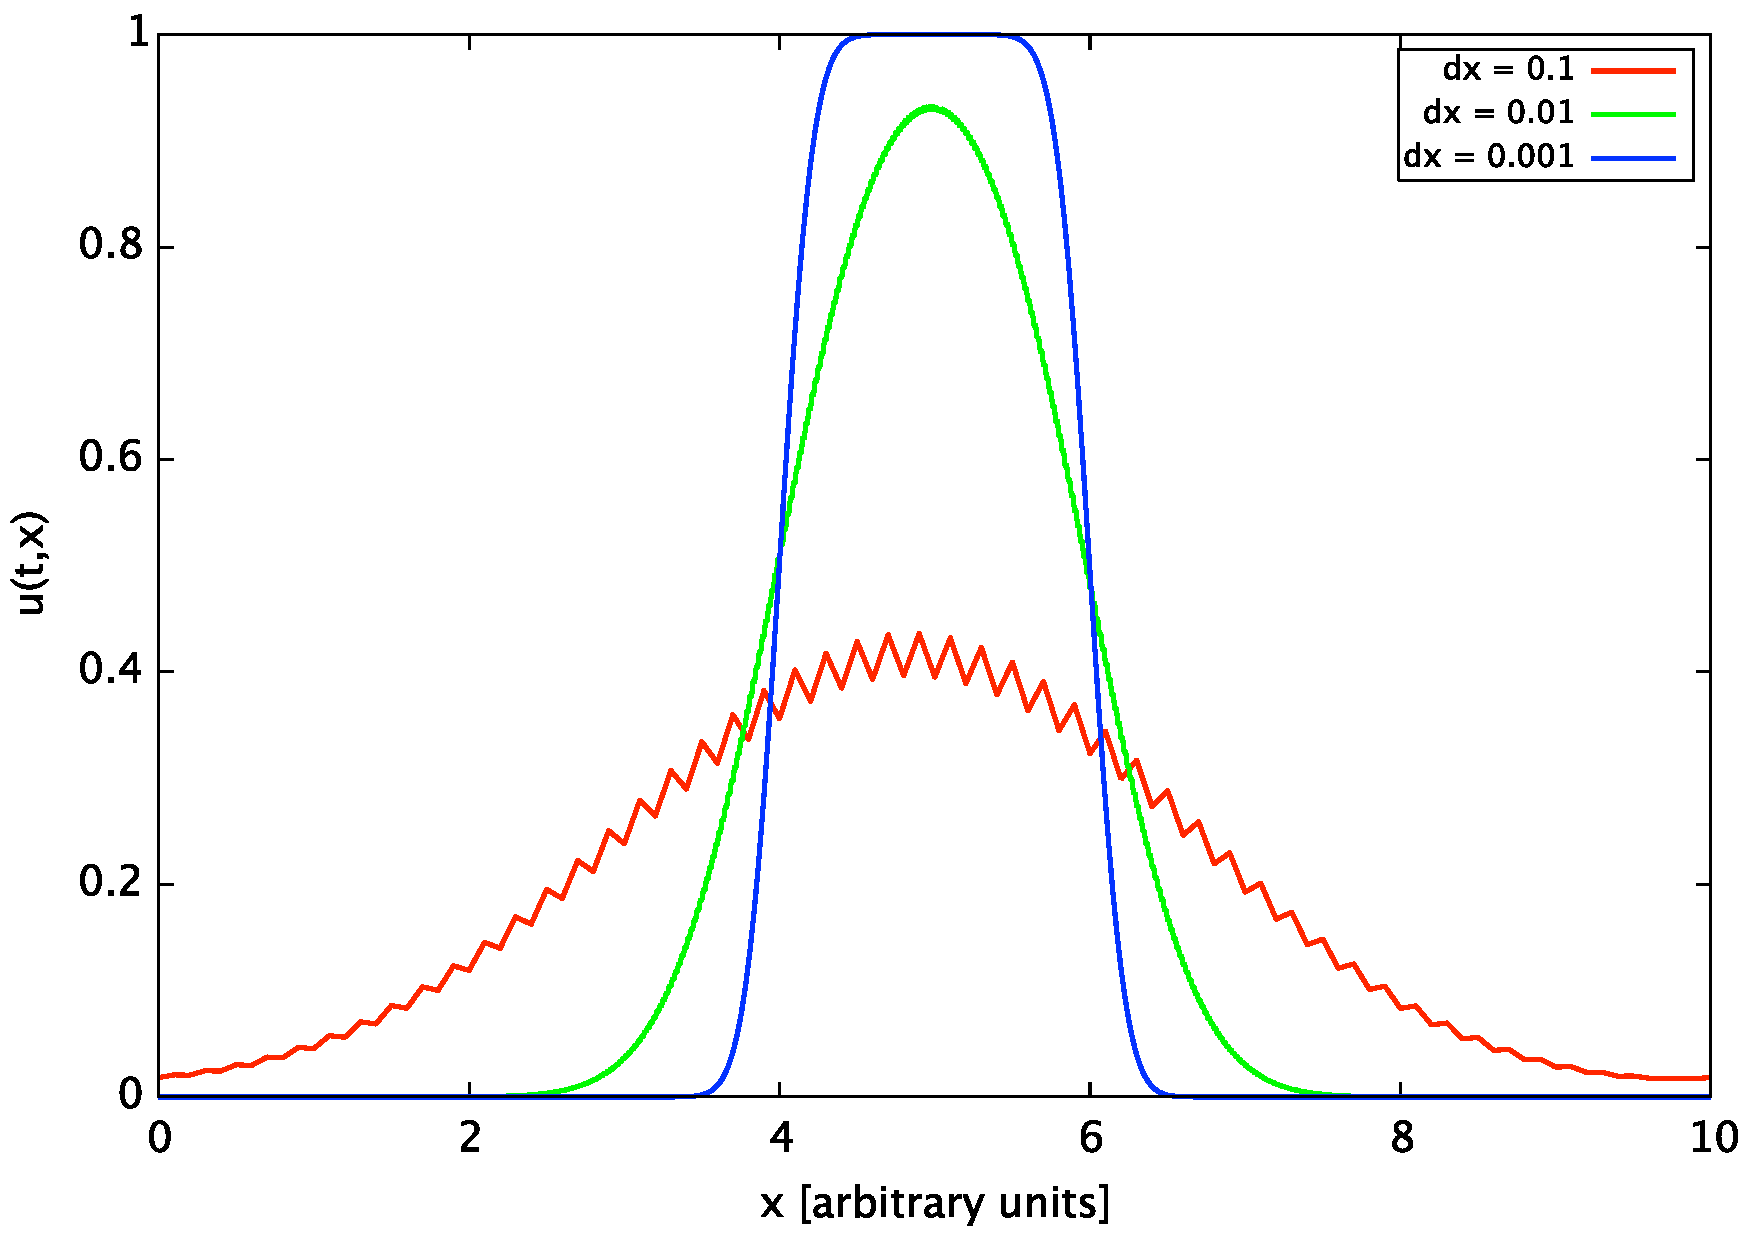
\includegraphics[scale=0.25]{good_img/lxfr_cf05_t20_s}}
\subfigure[$u(x,t=10)$ with $c_f=1$]
{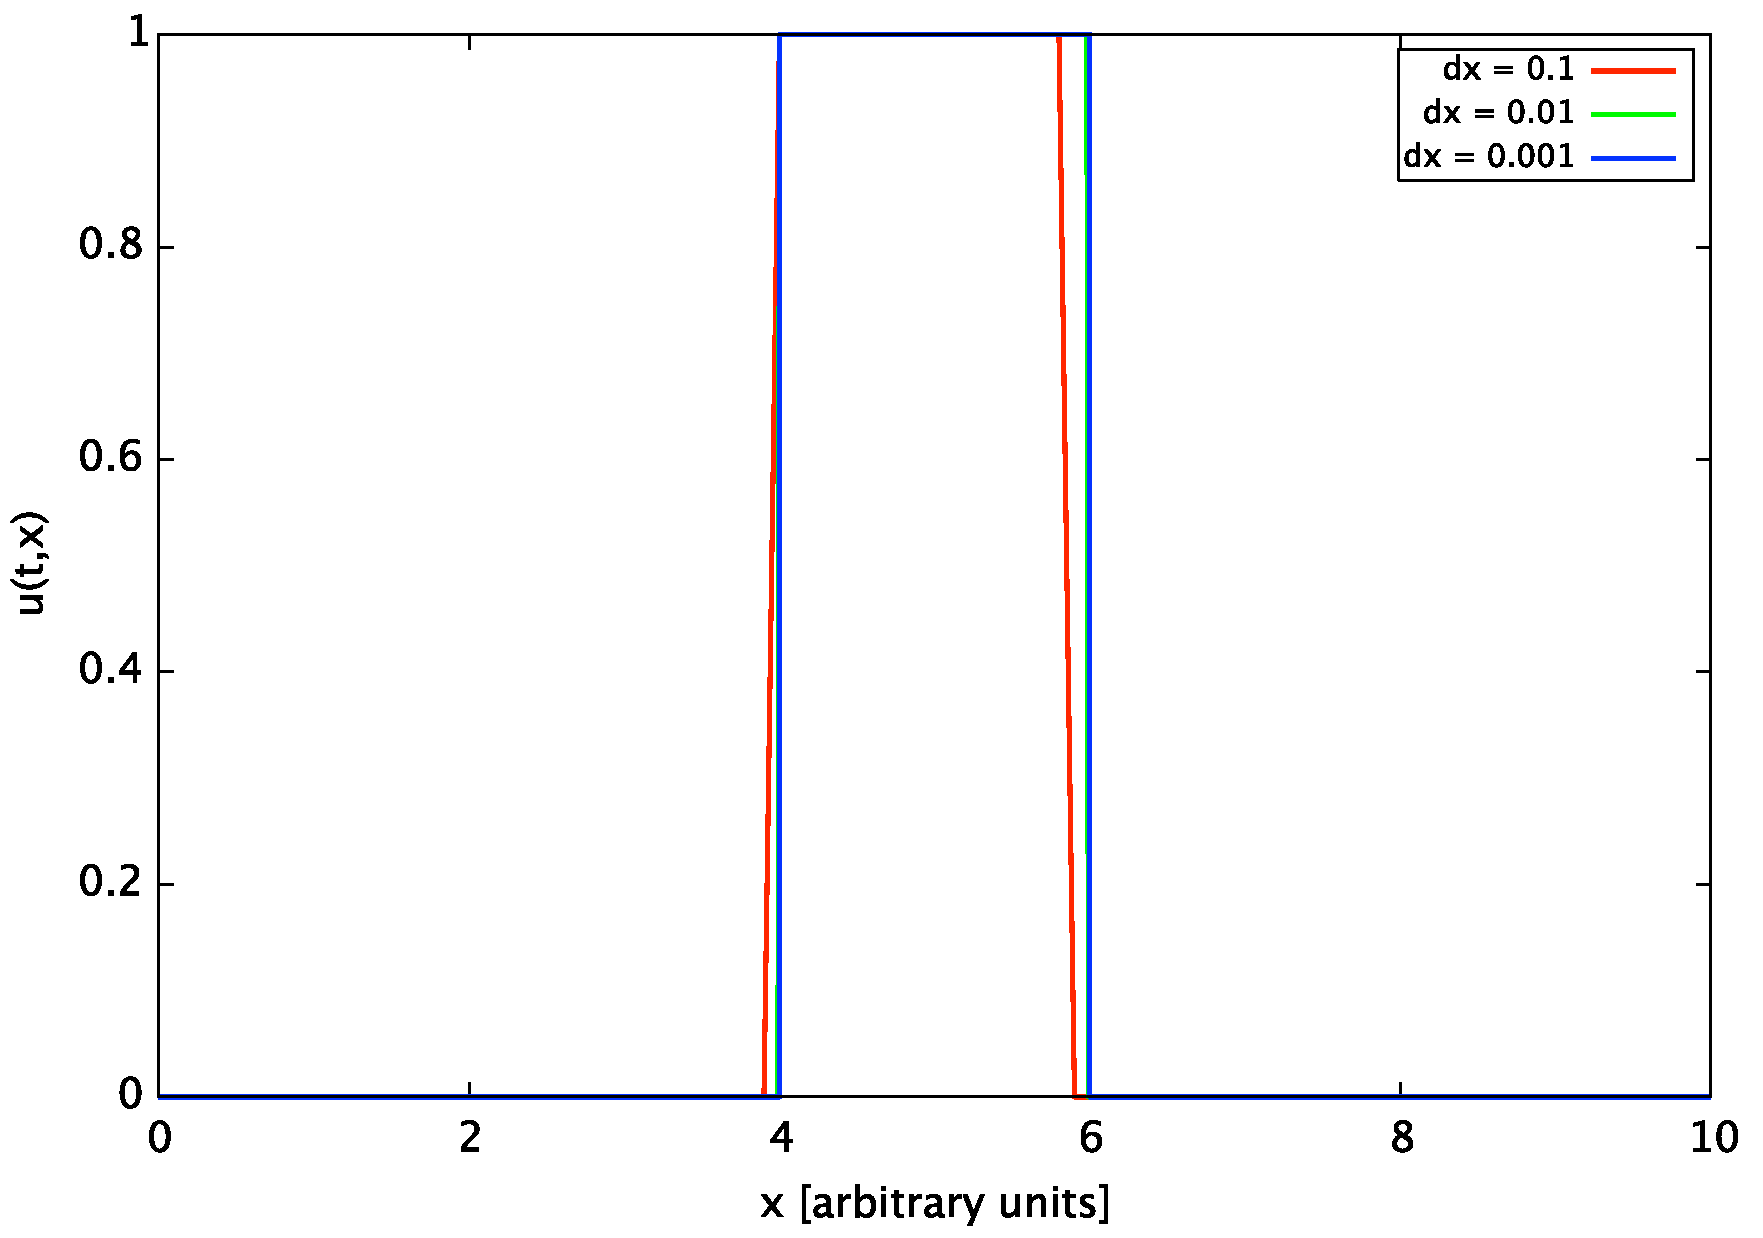
\includegraphics[scale=0.25]{good_img/lxfr_cf1_t10_s}}
\subfigure[$u(x,t=20)$ with $c_f=1$]
{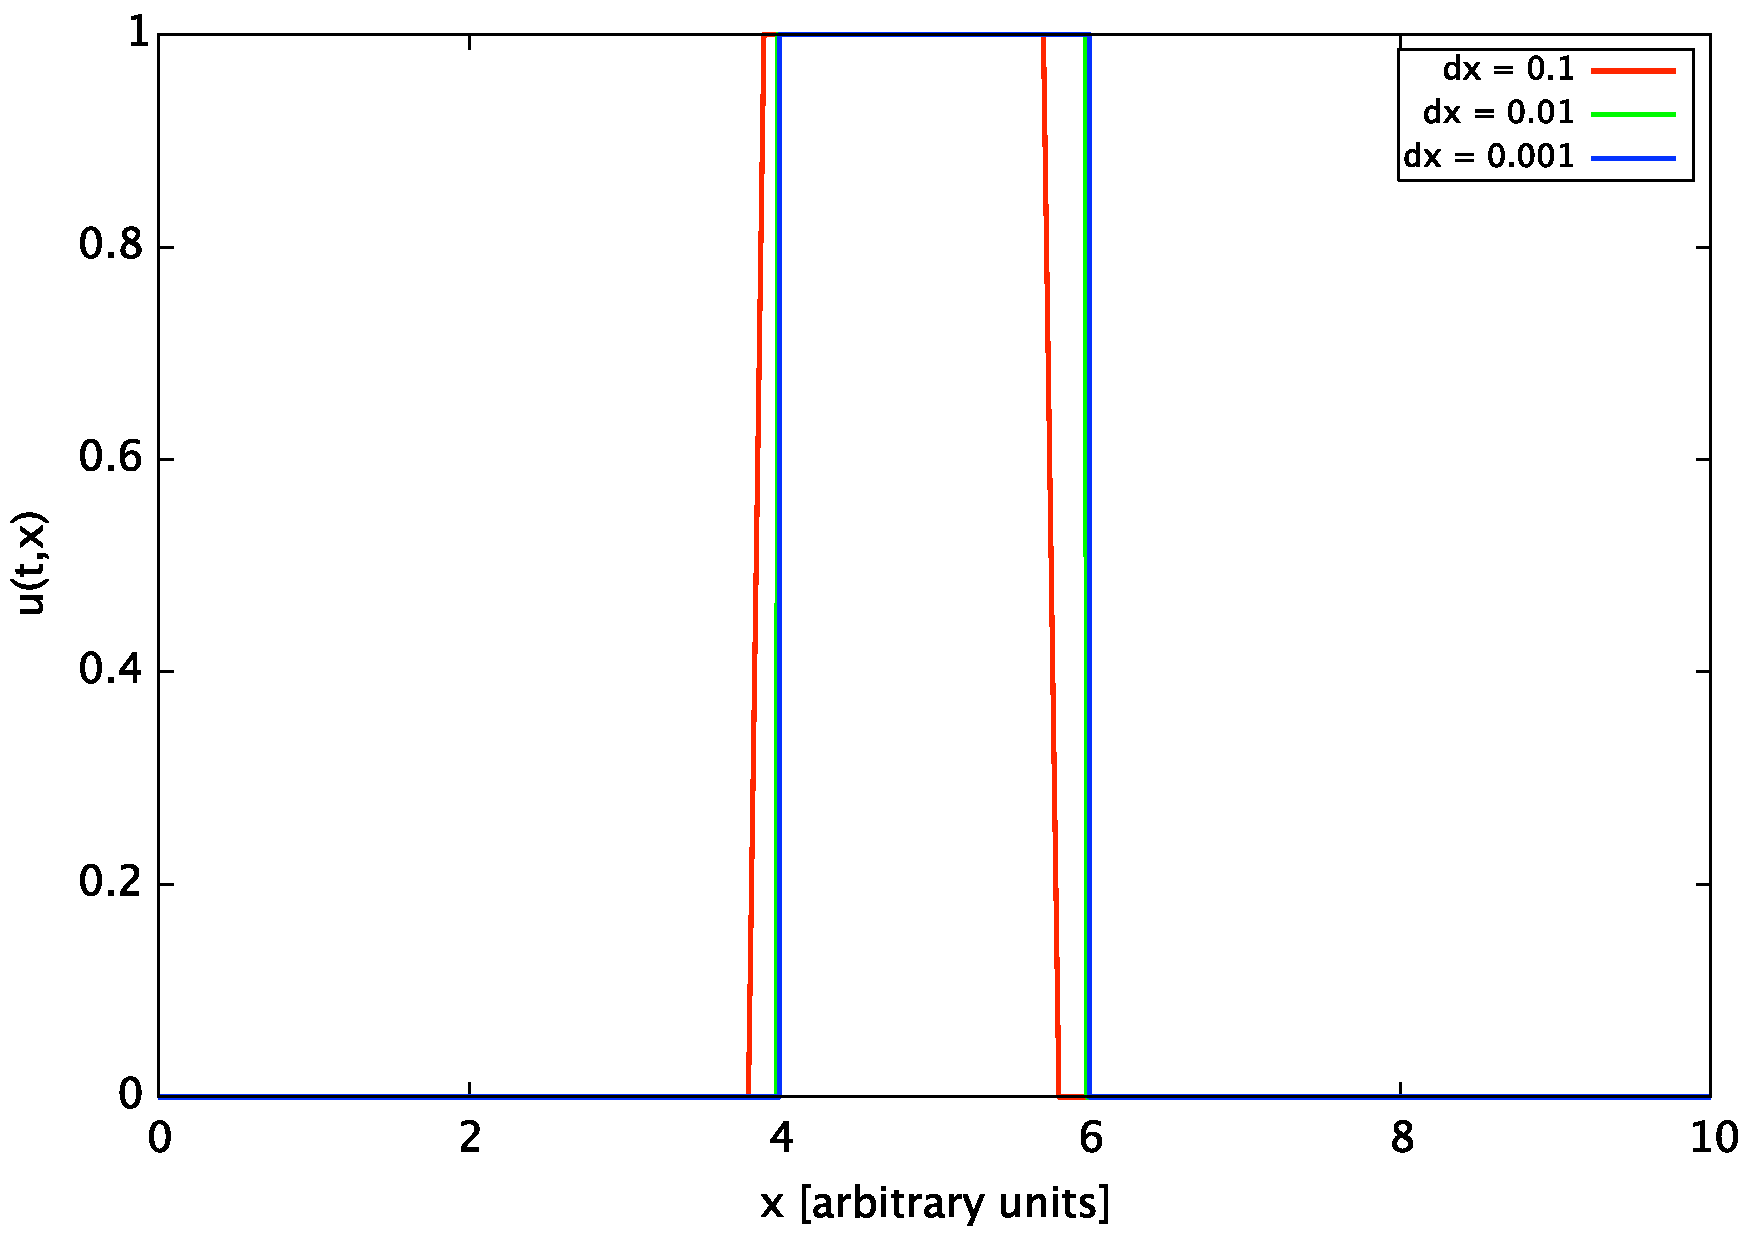
\includegraphics[scale=0.25]{good_img/lxfr_cf1_t20_s}}
\subfigure[L2-norm with $c_f=0.5$ and $\Delta x = 0.1$ for the Gaussian initial condition]
{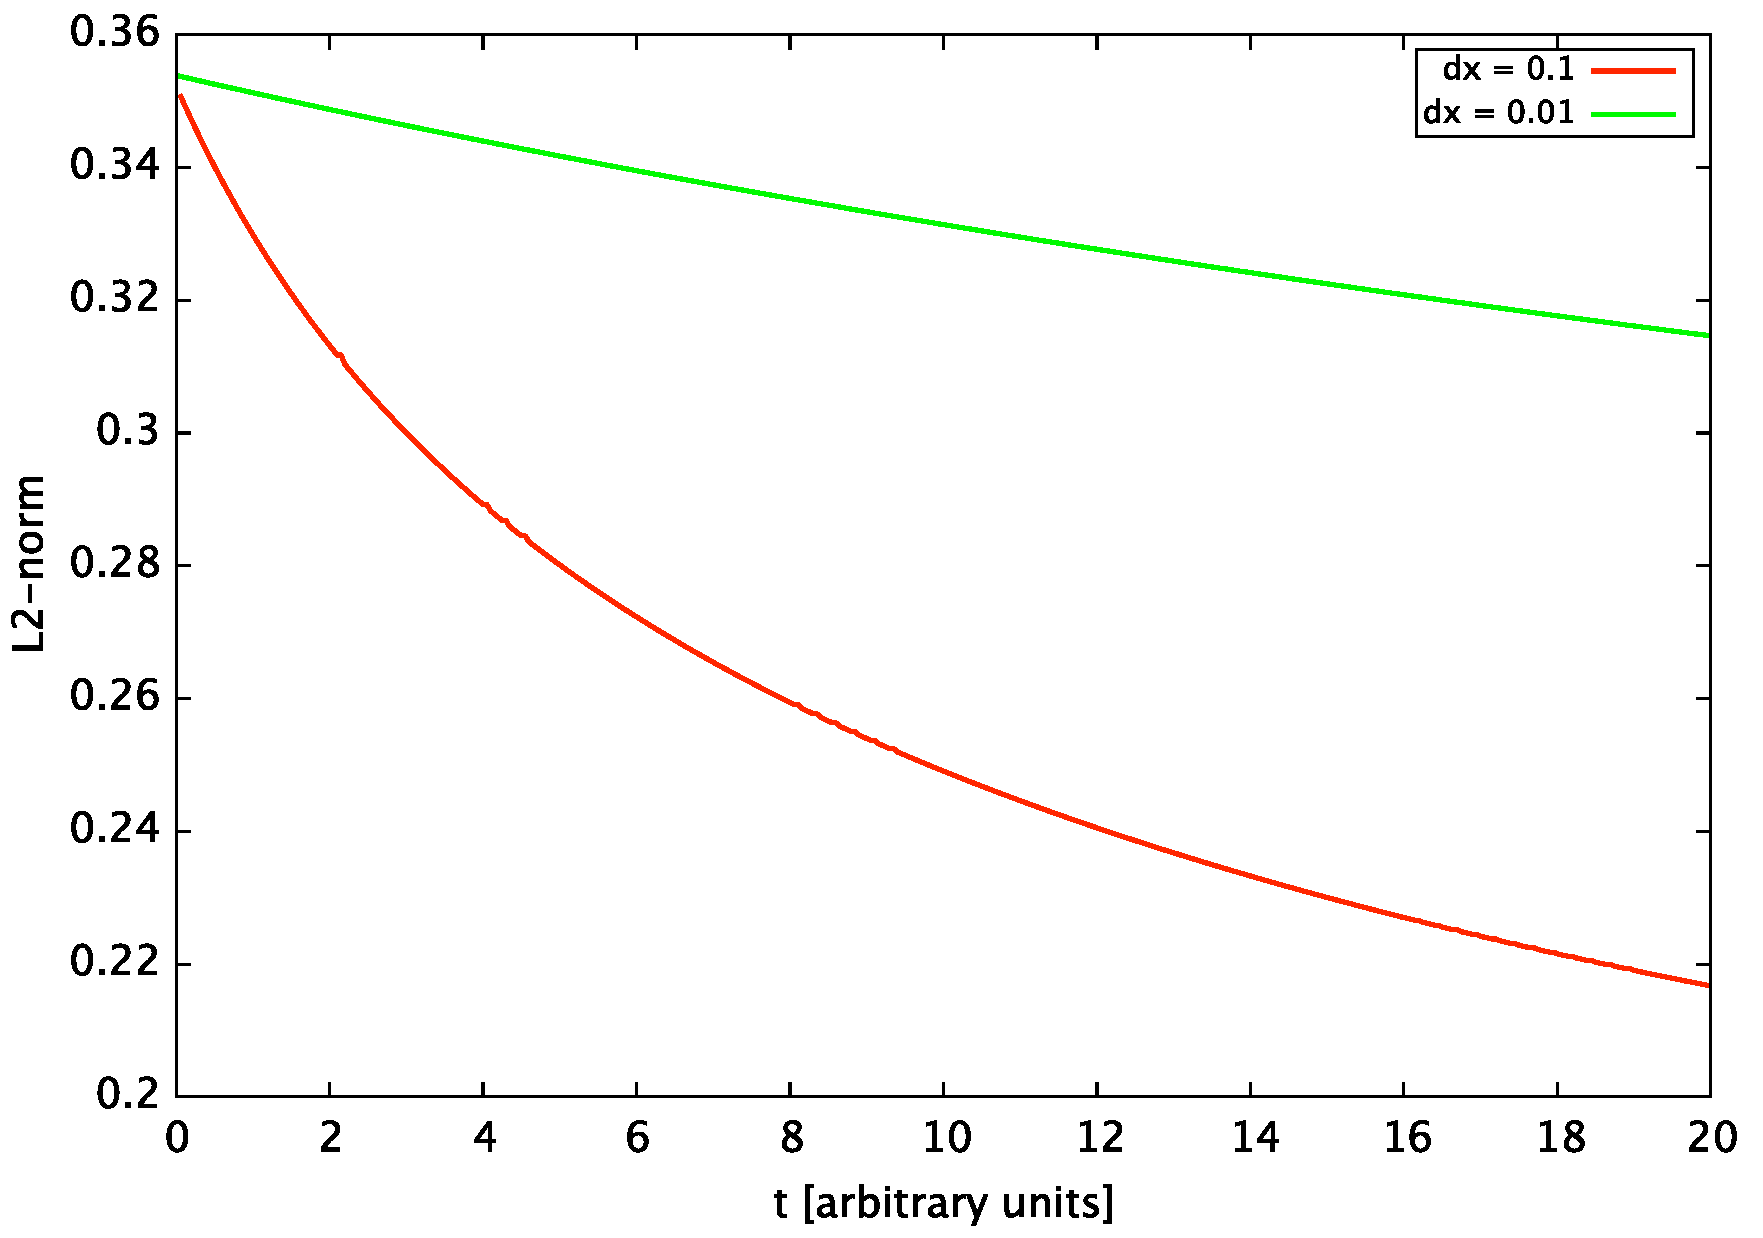
\includegraphics[scale=0.25]{good_img/lf_l2_g}}
\subfigure[L2-norm with $c_f=0.5$ and $\Delta x = 0.1$ for the square wave initial condition]
{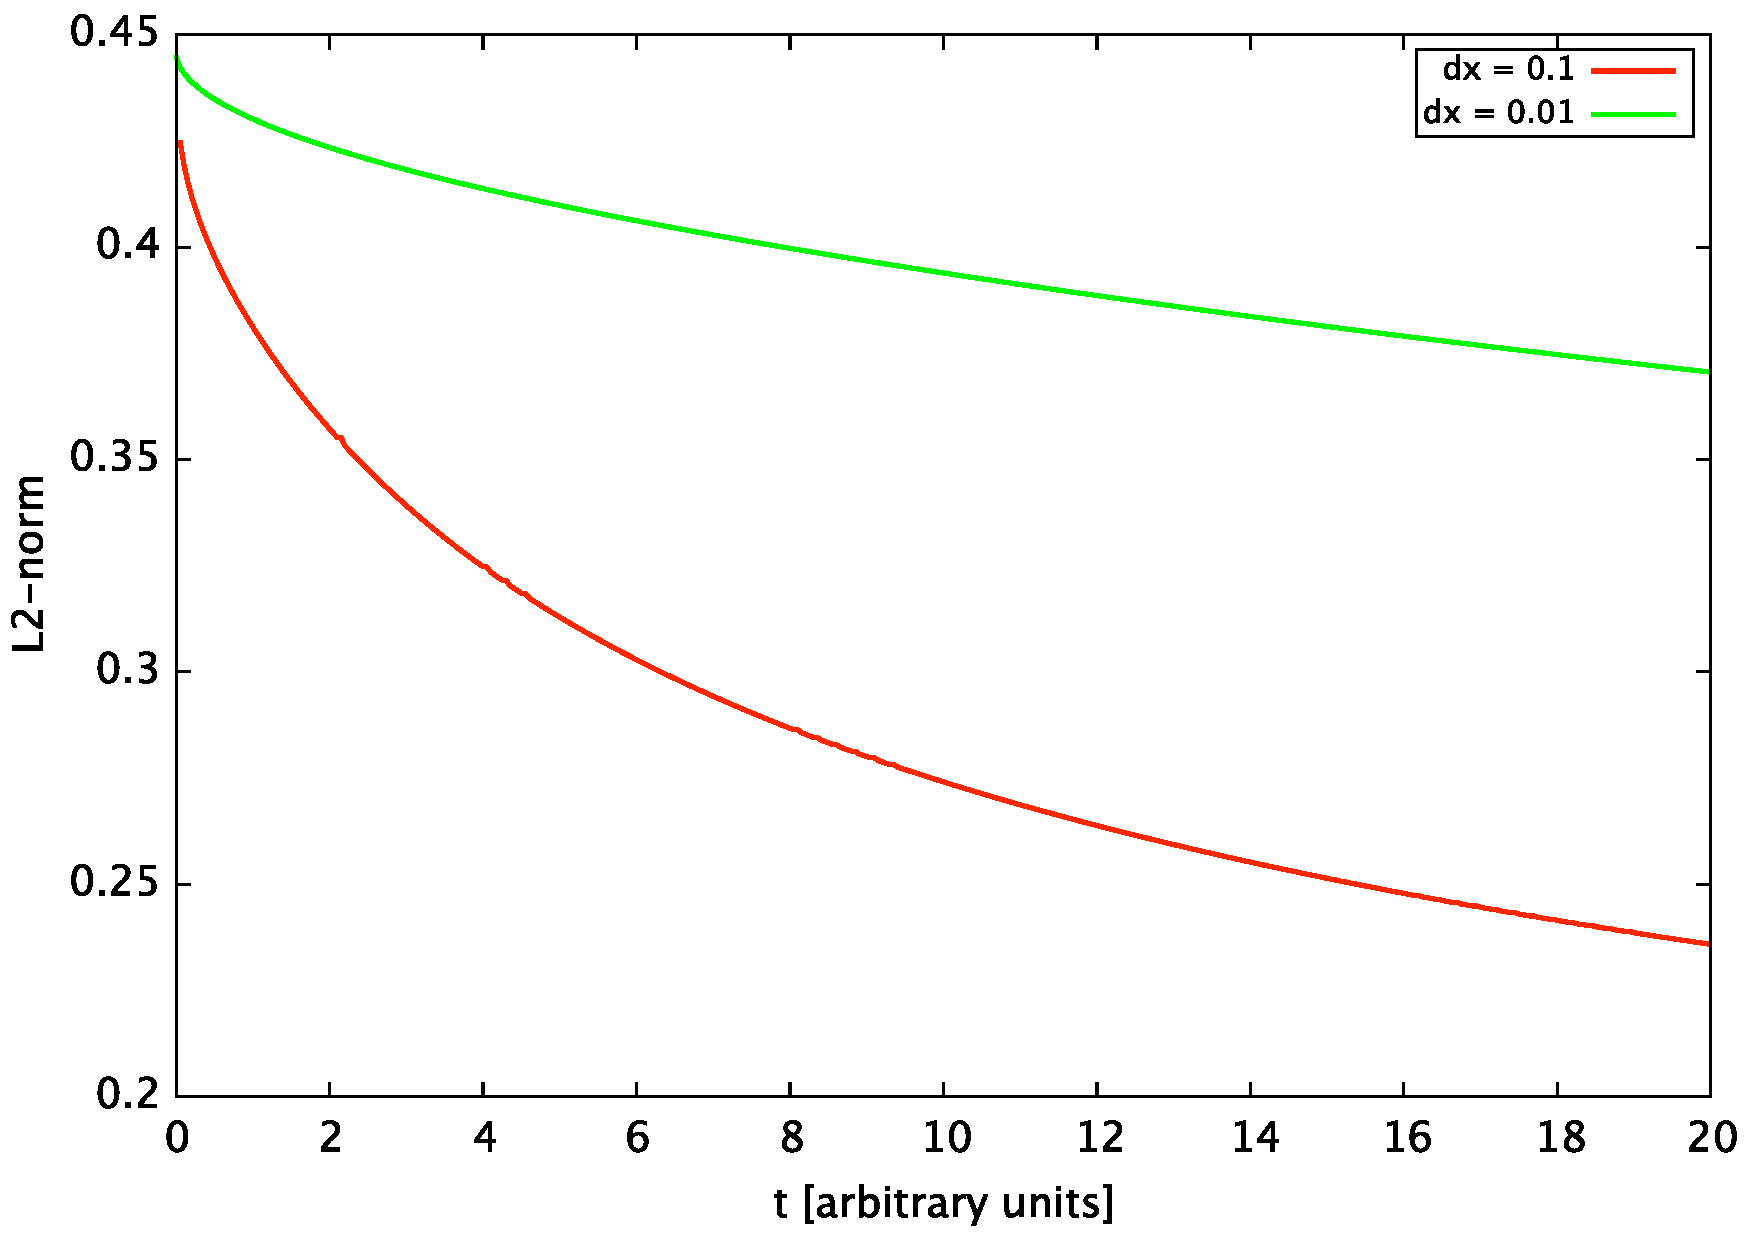
\includegraphics[scale=0.25]{good_img/lf_l2_s}}
\end{figure}\\
As expected, with $c_f=0.5$ the wave dissipates proportionally with $\Delta x$, while with $c_f= 1$ there is no dissipation whatsoever. Together with the other pictures also the plot of the L2-norms in the two different cases is shown (Fig. 1.27, 1.28). \\
\section{The Lax-Wendroff method}
The Lax-Wendroff method is obtained combining Leapfrog and Lax-Friedrichs methods. The algorithm is given by
\begin{equation}\label{lw}
u_j^{n+1}= u_j^n - a\frac{\Delta t}{2 \Delta x} (u_{j+1}^n - u_{j-1}^n) + \frac{a^2 \Delta t^2}{2 \Delta x^2}(u_{j+1}^n - 2u_j^n + u_{j-1}^n)
\end{equation} 
which is evidently a second order method with no dependence on the $n-1$ step. Even if the method is stable under the Von Neumann condition, it still has a dissipative effect. In fact, going back from \eqref{lw} to the differential equation we obtain
\begin{equation}
u_t + a u_x = -\frac{1}{6}a\Delta x^2 \left( 1- a^2 \frac{\Delta t^2}{\Delta x^2} \right)u_{xxx} + a^2 \frac{\Delta t \Delta x^2}{24} \left( 1- a^2 \frac{\Delta t^2}{\Delta x^2} \right)u_{xxxx}
\end{equation}
showing that the method added a dispersive term (the first one on the right-hand side) proportional to $\Delta x^2$ and a dissipative term proportional to $\Delta x^3$. It is also evident that for $c_f=1$  dispersion and dissipation become zero. Let us look now at the solutions obtained with initial condition (1) (Fig. 1.29 - 1.32):
\begin{figure}[!h]
\begin{center}
\subfigure[$u(x,t=10)$ with $c_f=0.5$]{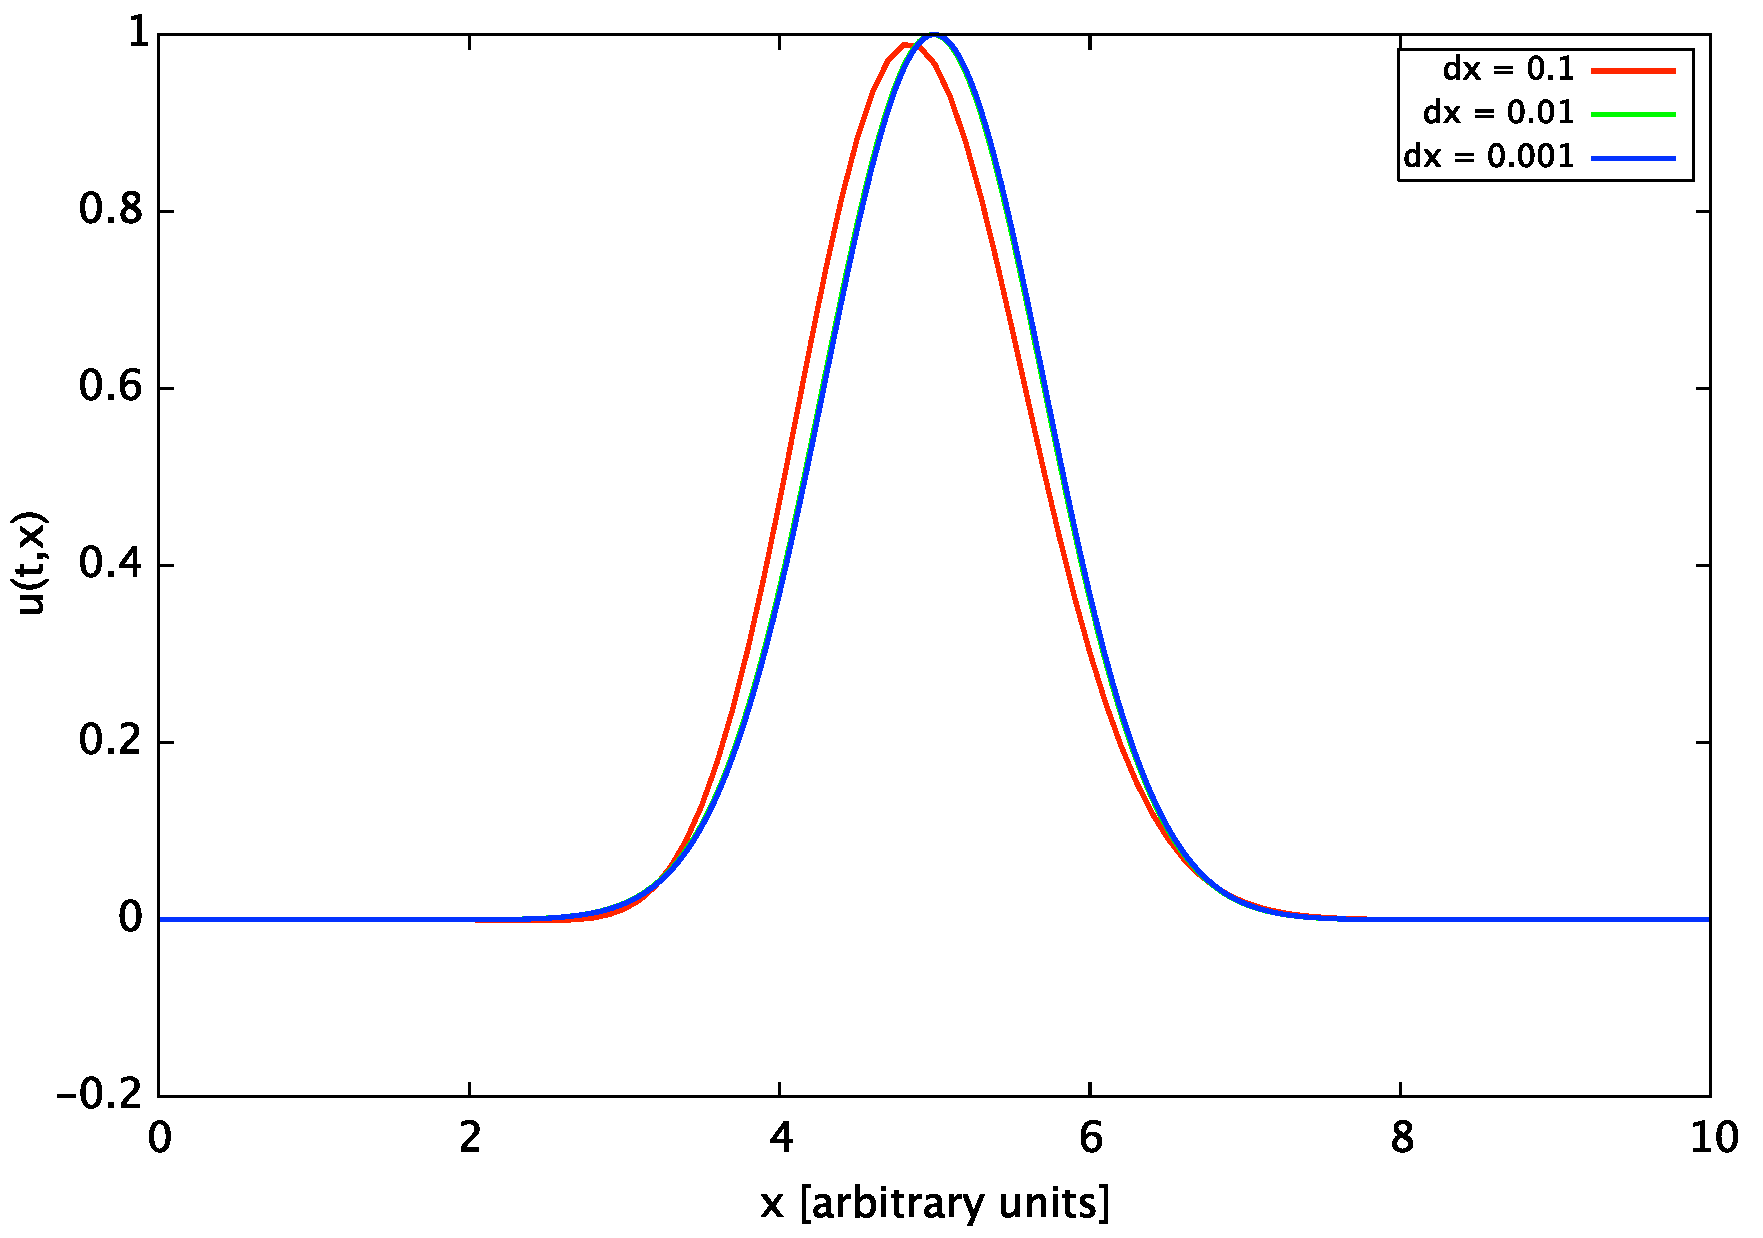
\includegraphics[scale=0.25]{good_img/lw_cf05_t10_g}} 
\subfigure[$u(x,t=10)$ with $c_f=1$d]{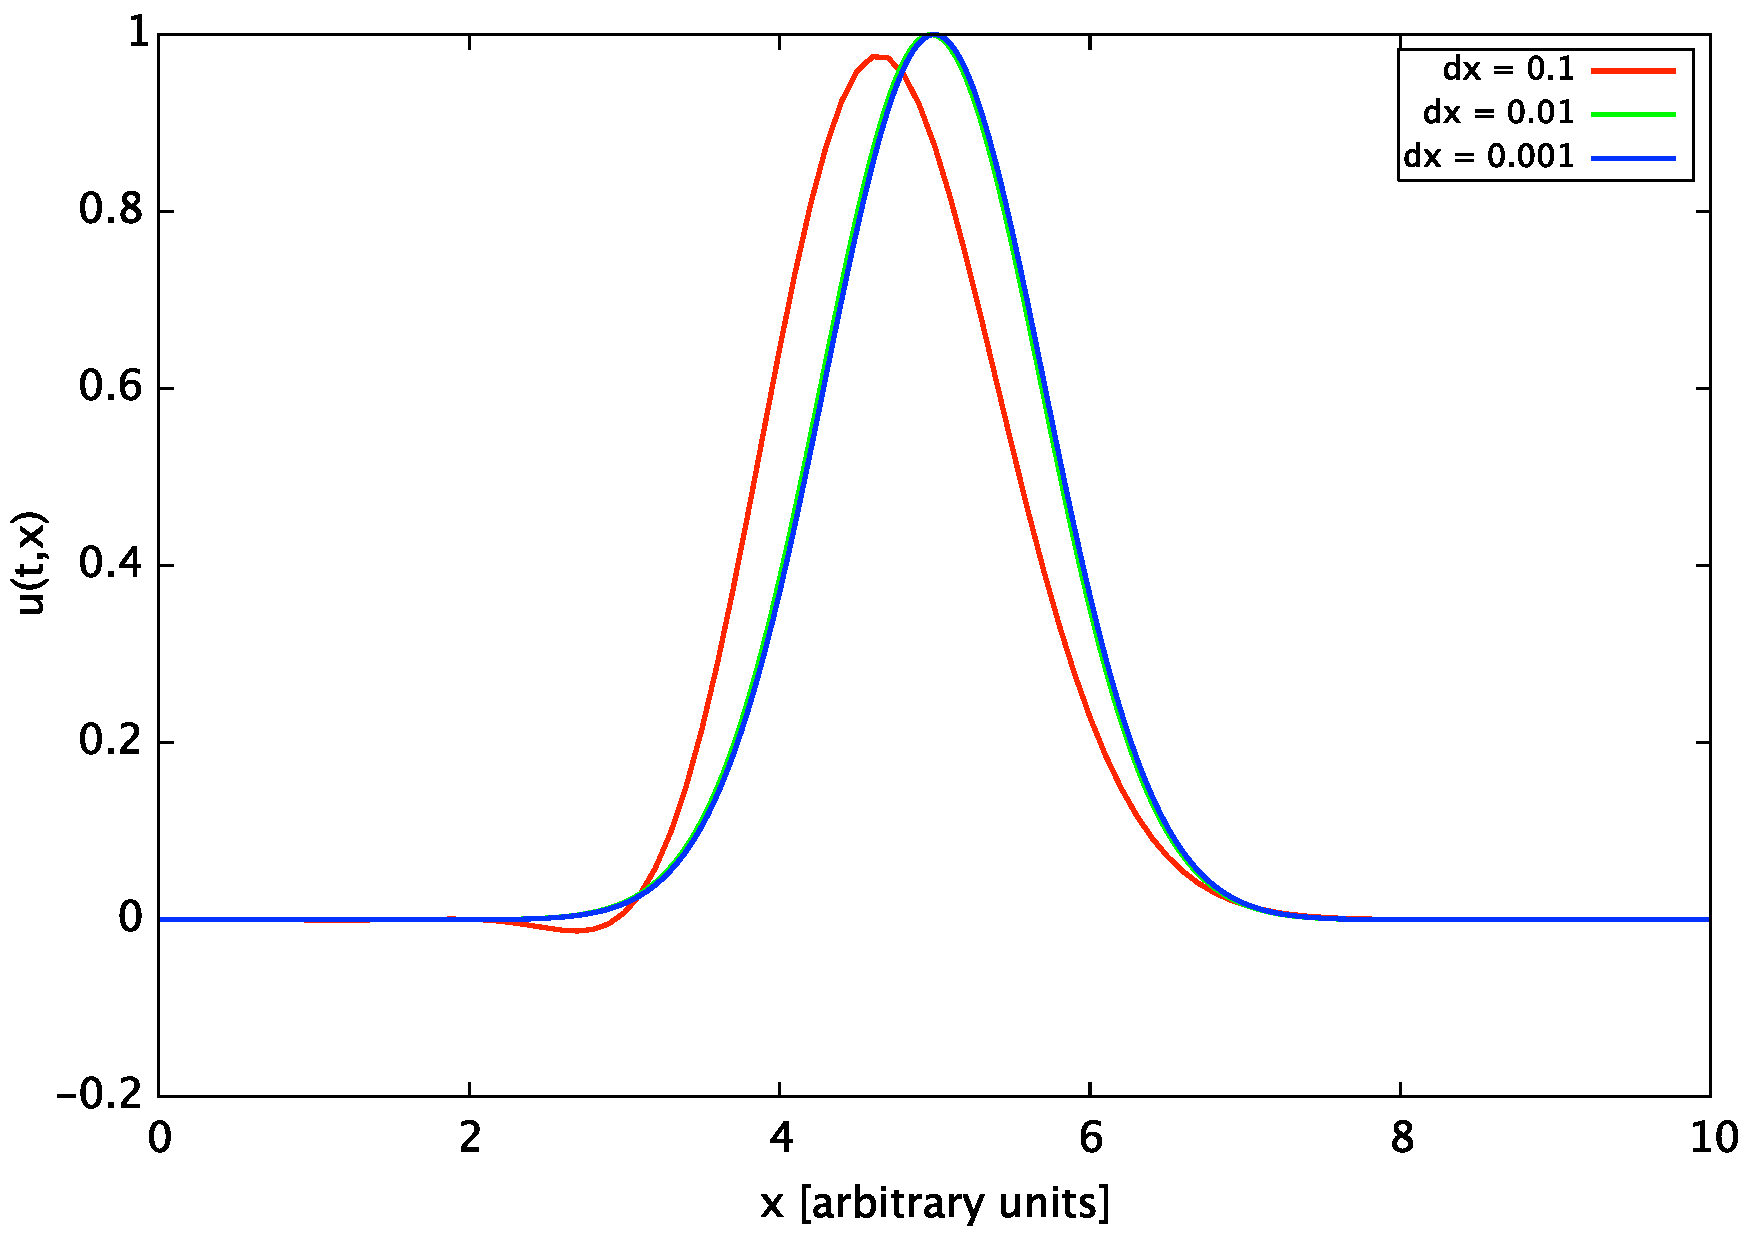
\includegraphics[scale=0.25]{good_img/lw_cf05_t20_g}}
\subfigure[$u(x,t=20)$ with $c_f=0.5$]{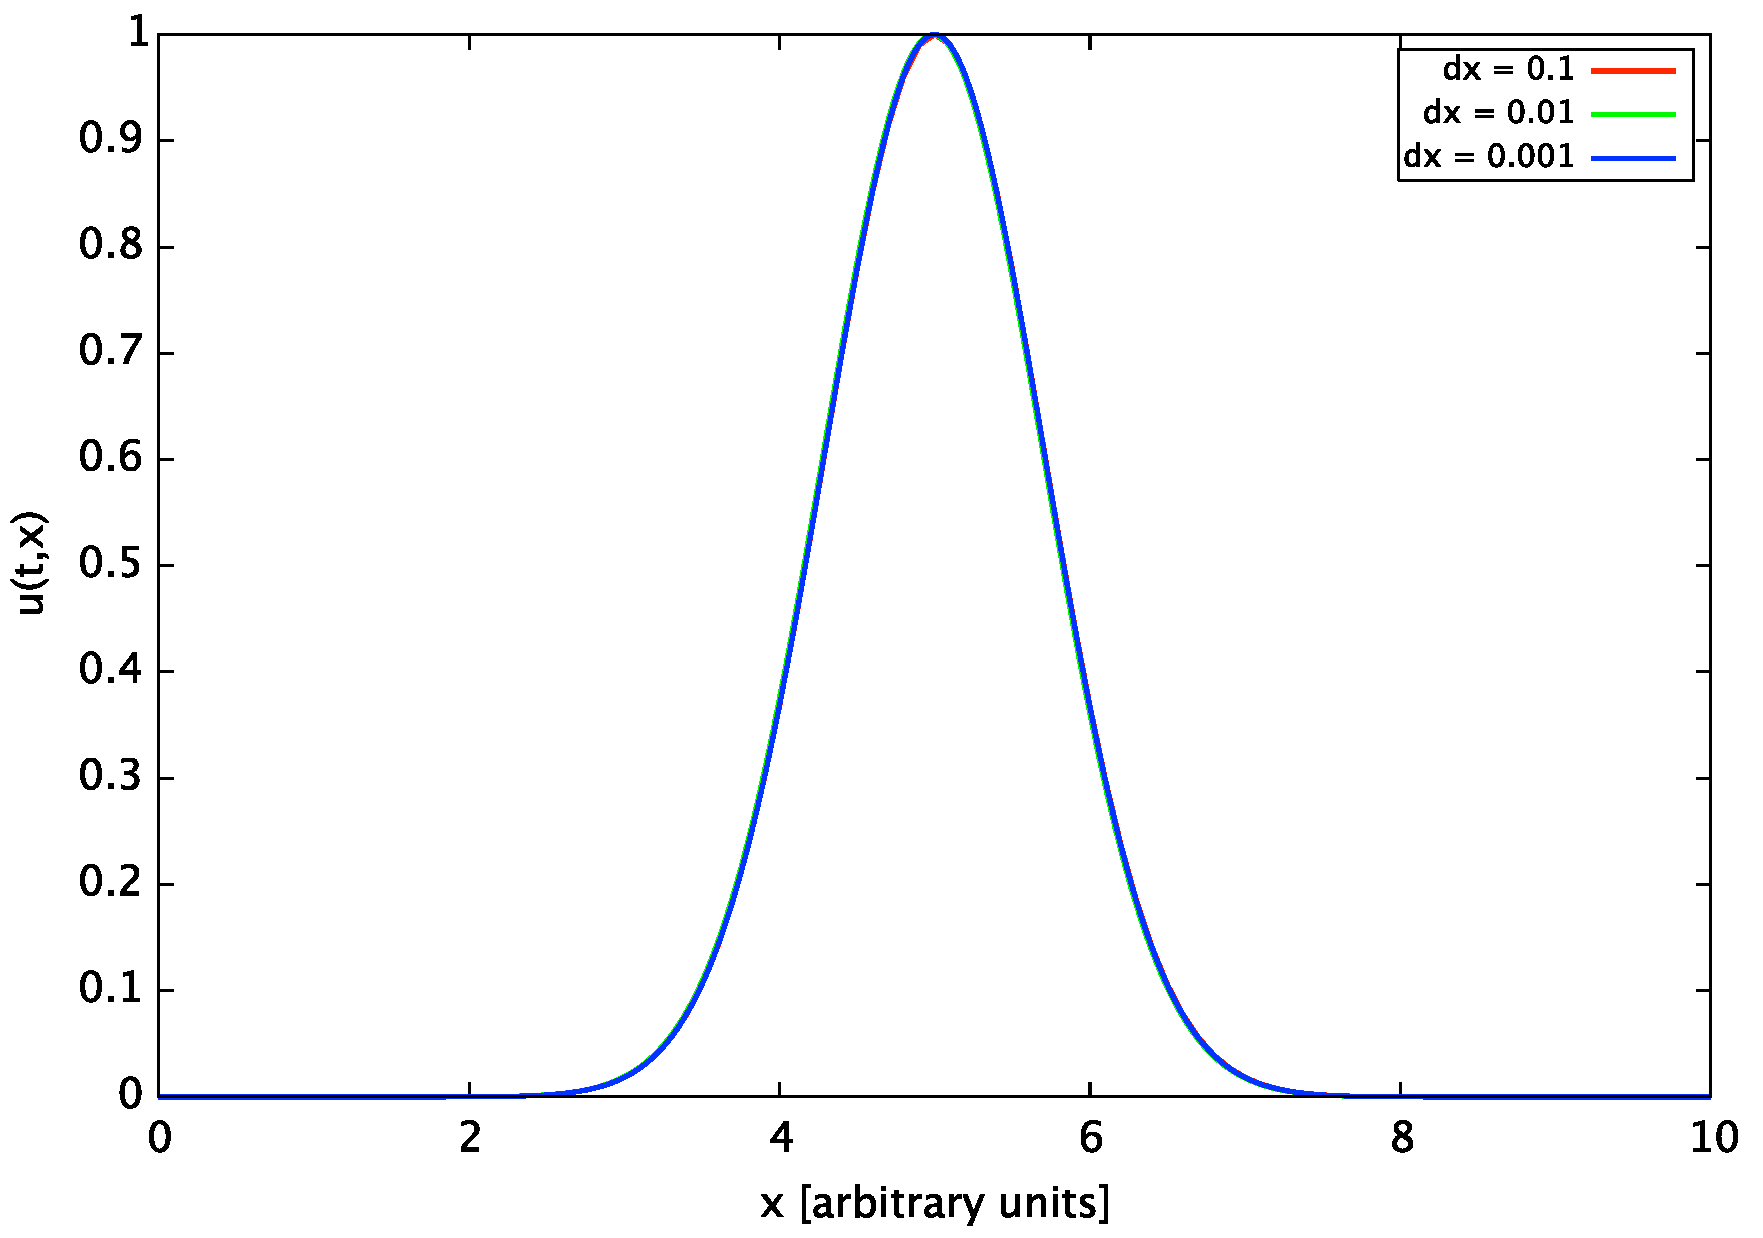
\includegraphics[scale=0.25]{good_img/fig121}} 
\subfigure[$u(x,t=20)$ with $c_f=1$]{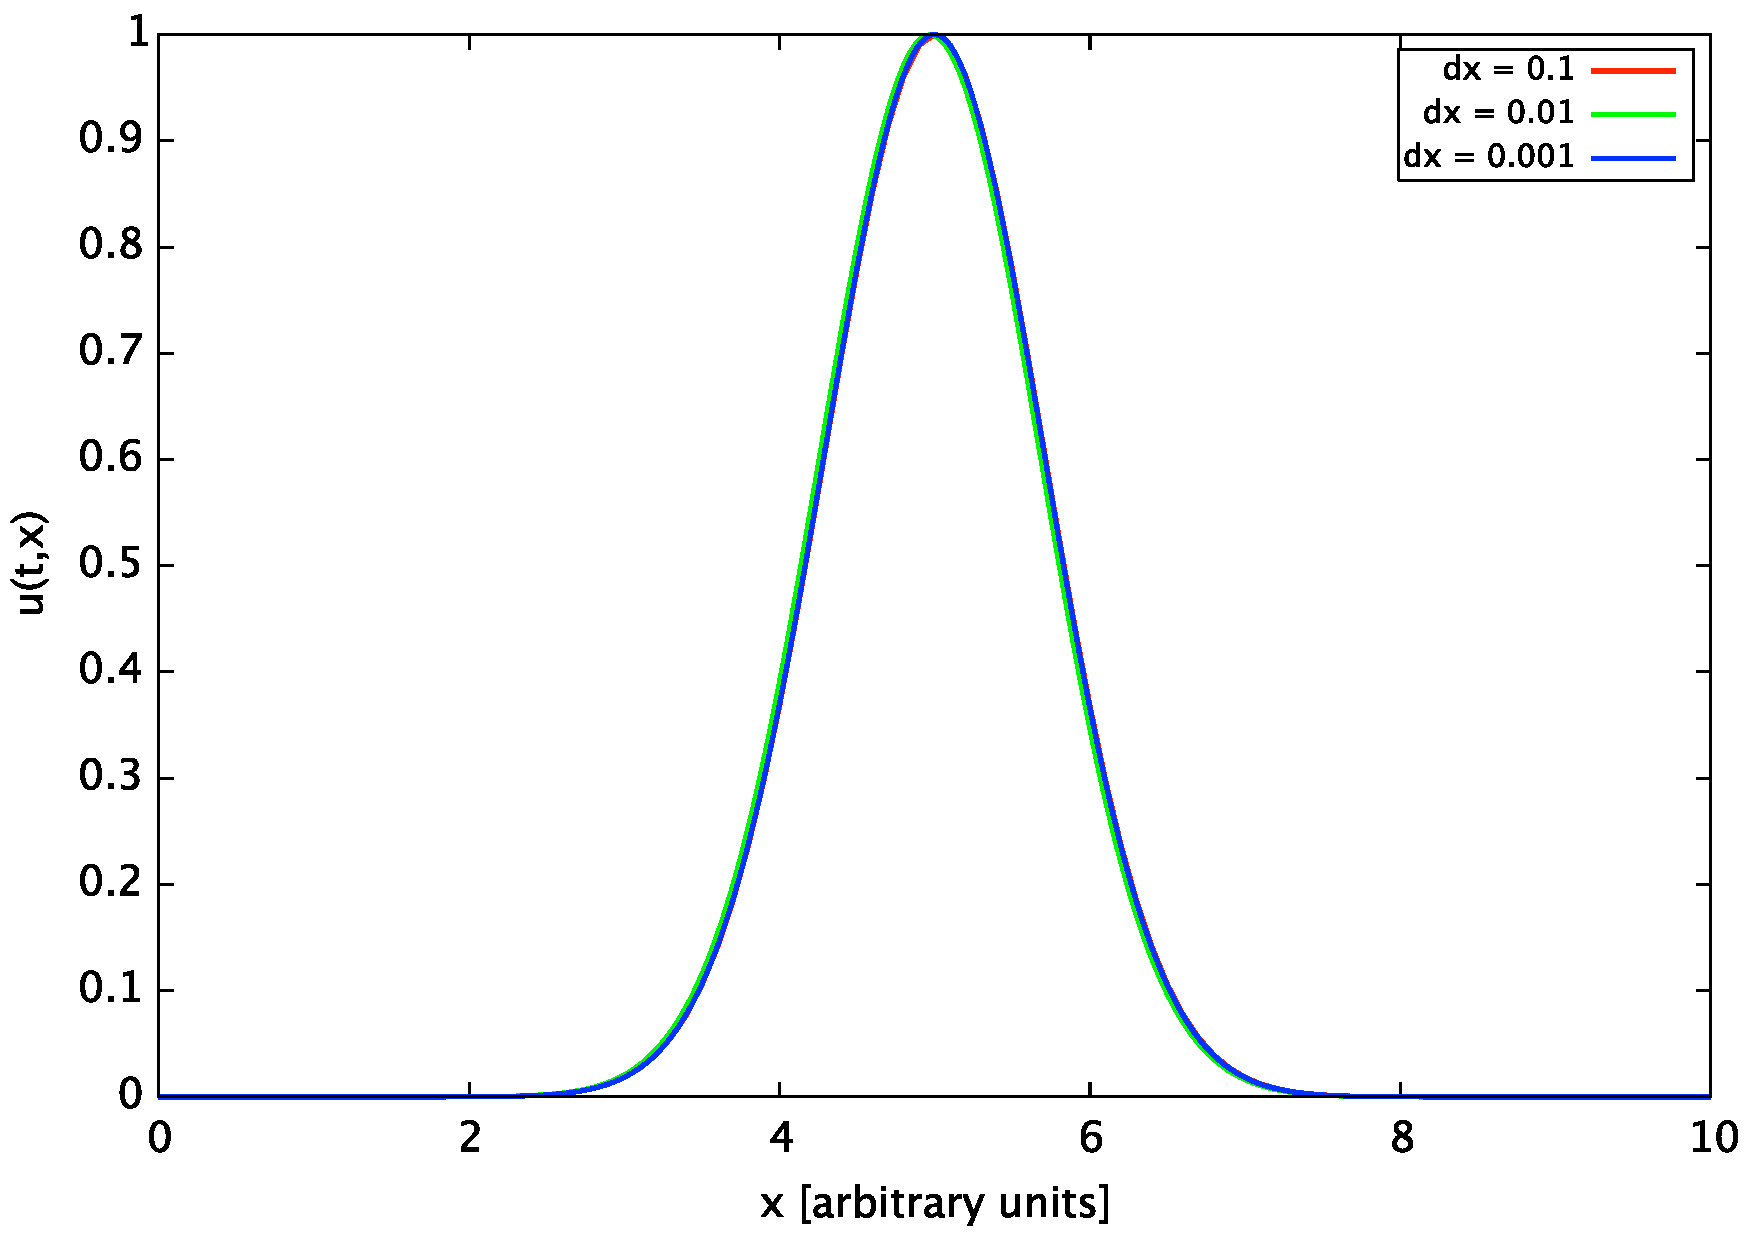
\includegraphics[scale=0.25]{good_img/fig122}}
\subfigure[$u(x,t=10)$ with $c_f=0.5$]{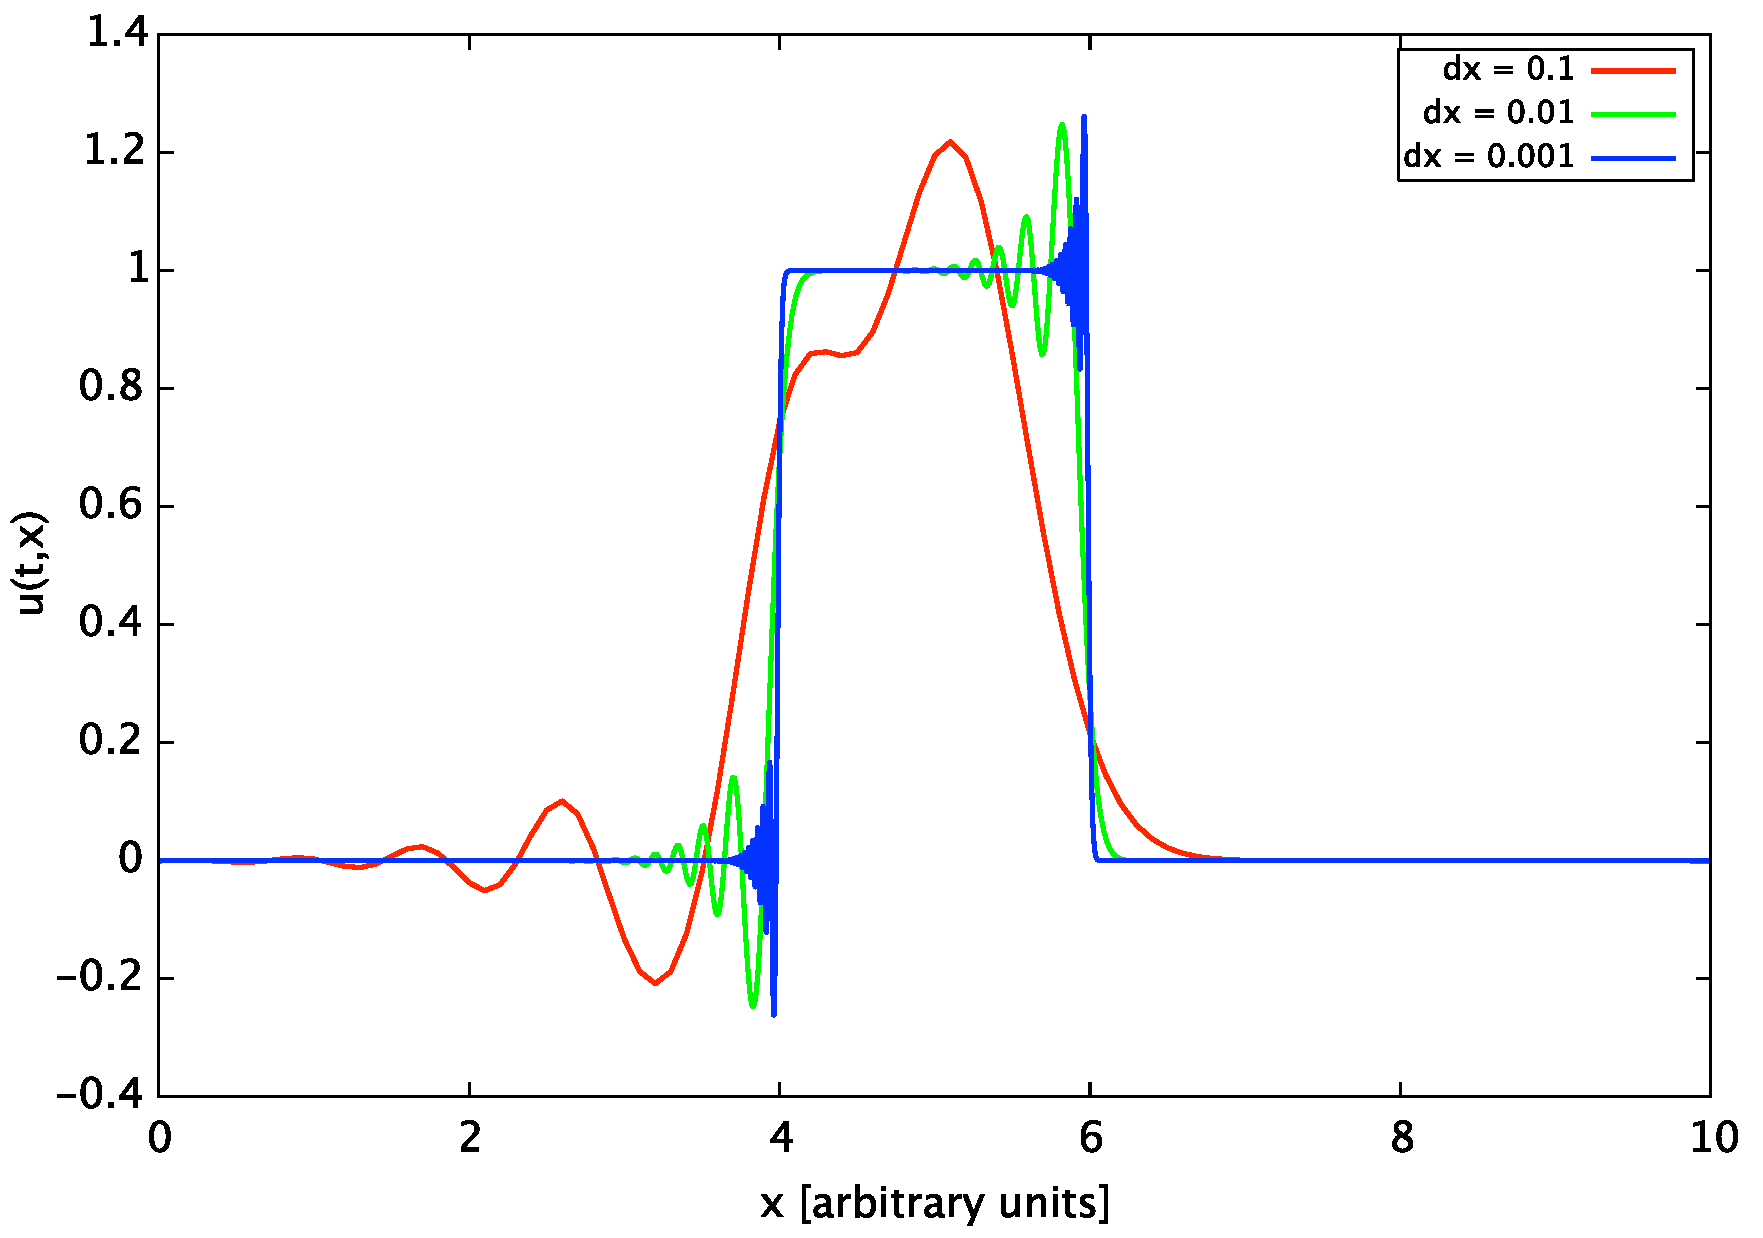
\includegraphics[scale=0.25]{good_img/lw_cf05_t10_s} }
\subfigure[$u(x,t=20)$ with $c_f=0.5$]{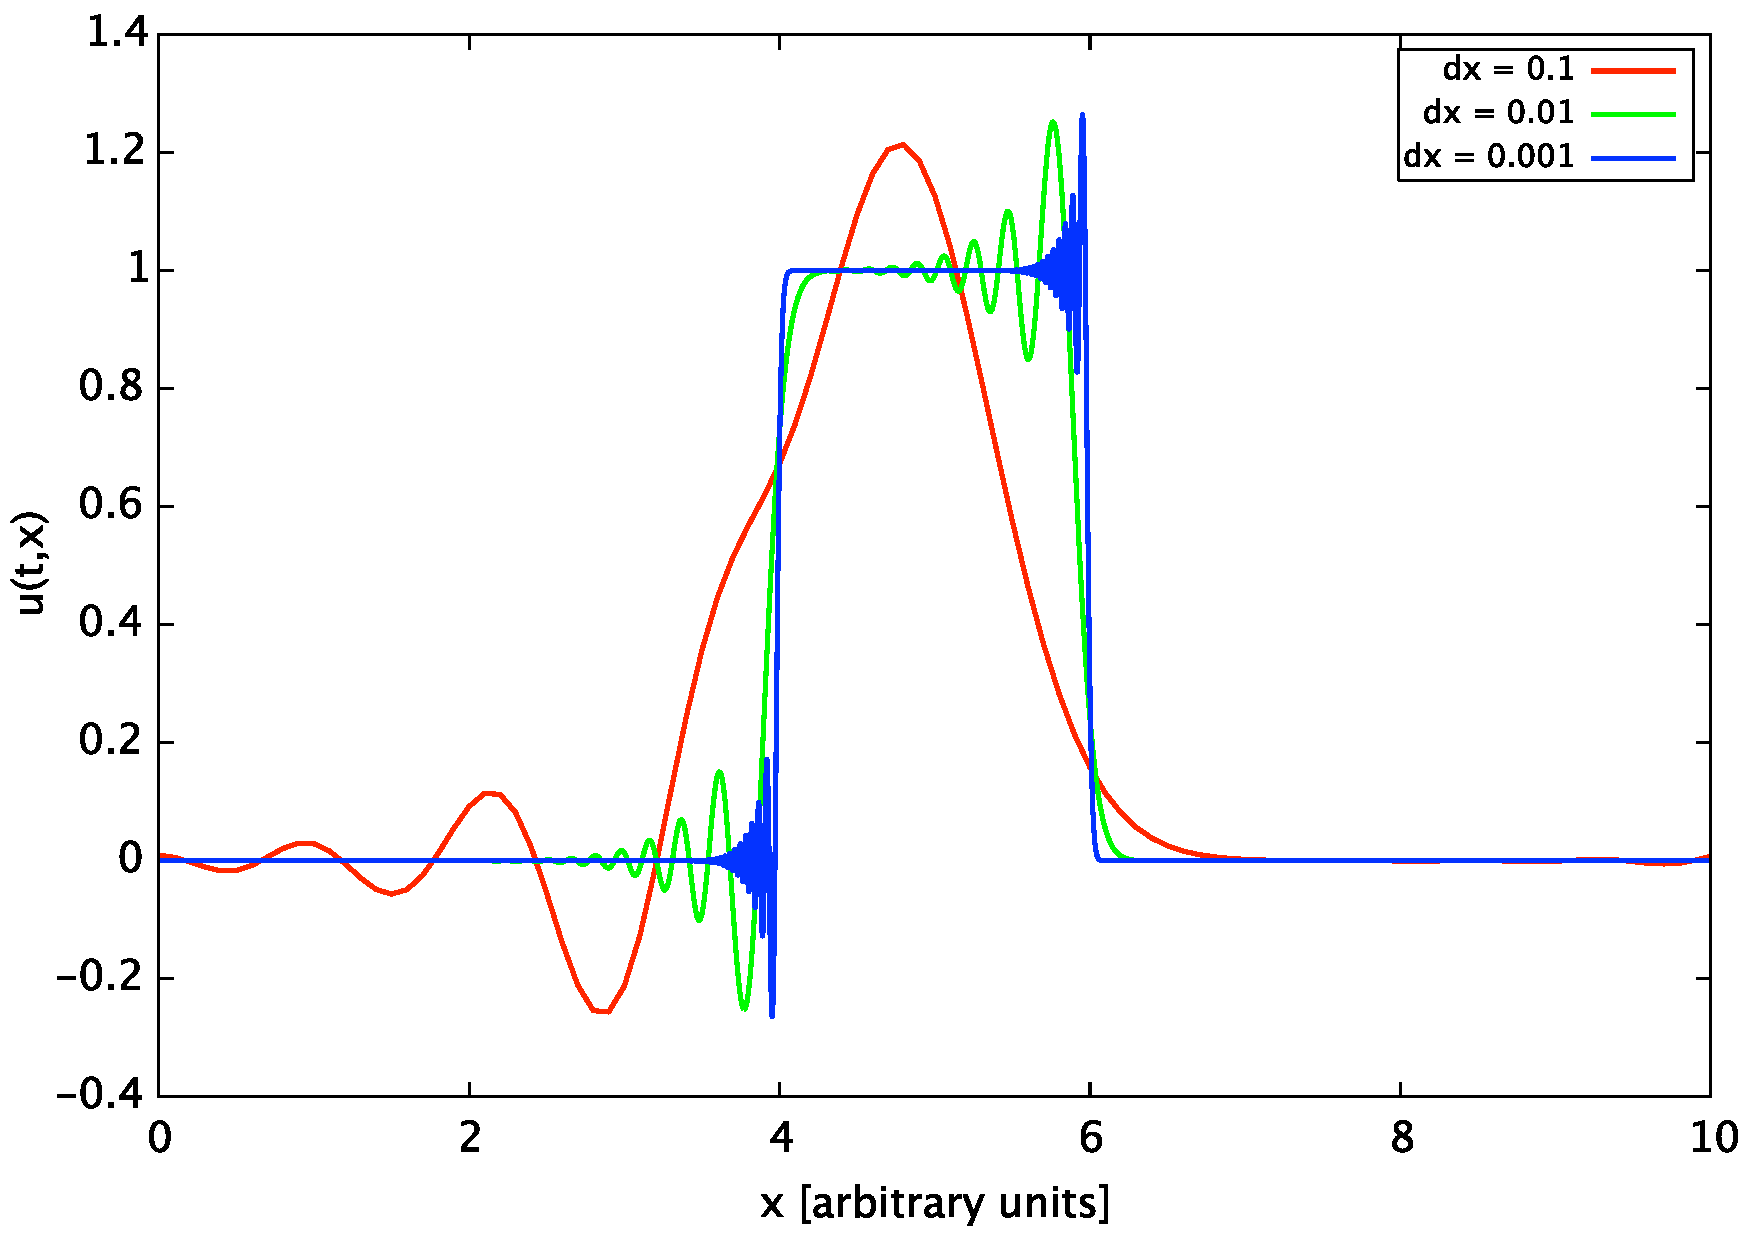
\includegraphics[scale=0.25]{good_img/lw_cf05_t20_s}}
\end{center}
\end{figure}\\
The obtained results underline what we expected on theoretical grounds: the dissipation is sensibly smaller than the one of Leapfrog, making clear the fact that now the dissipative effect is cubic in the mesh step and not linear anymore. For the evolution of initial condition (2) different results have been obtained (Fig. 1.33 - 1.36). Here the dissipative effect of the method become clear, destroying the solution in the case of $\Delta x \geq 0.1$ and $c_f = 0.5$ and generating cuspids in correspondence to the discontinuities of the square wave.
\begin{figure}[!h]
\begin{center}
\subfigure[$u(x,t=10)$ with $c_f=1$]{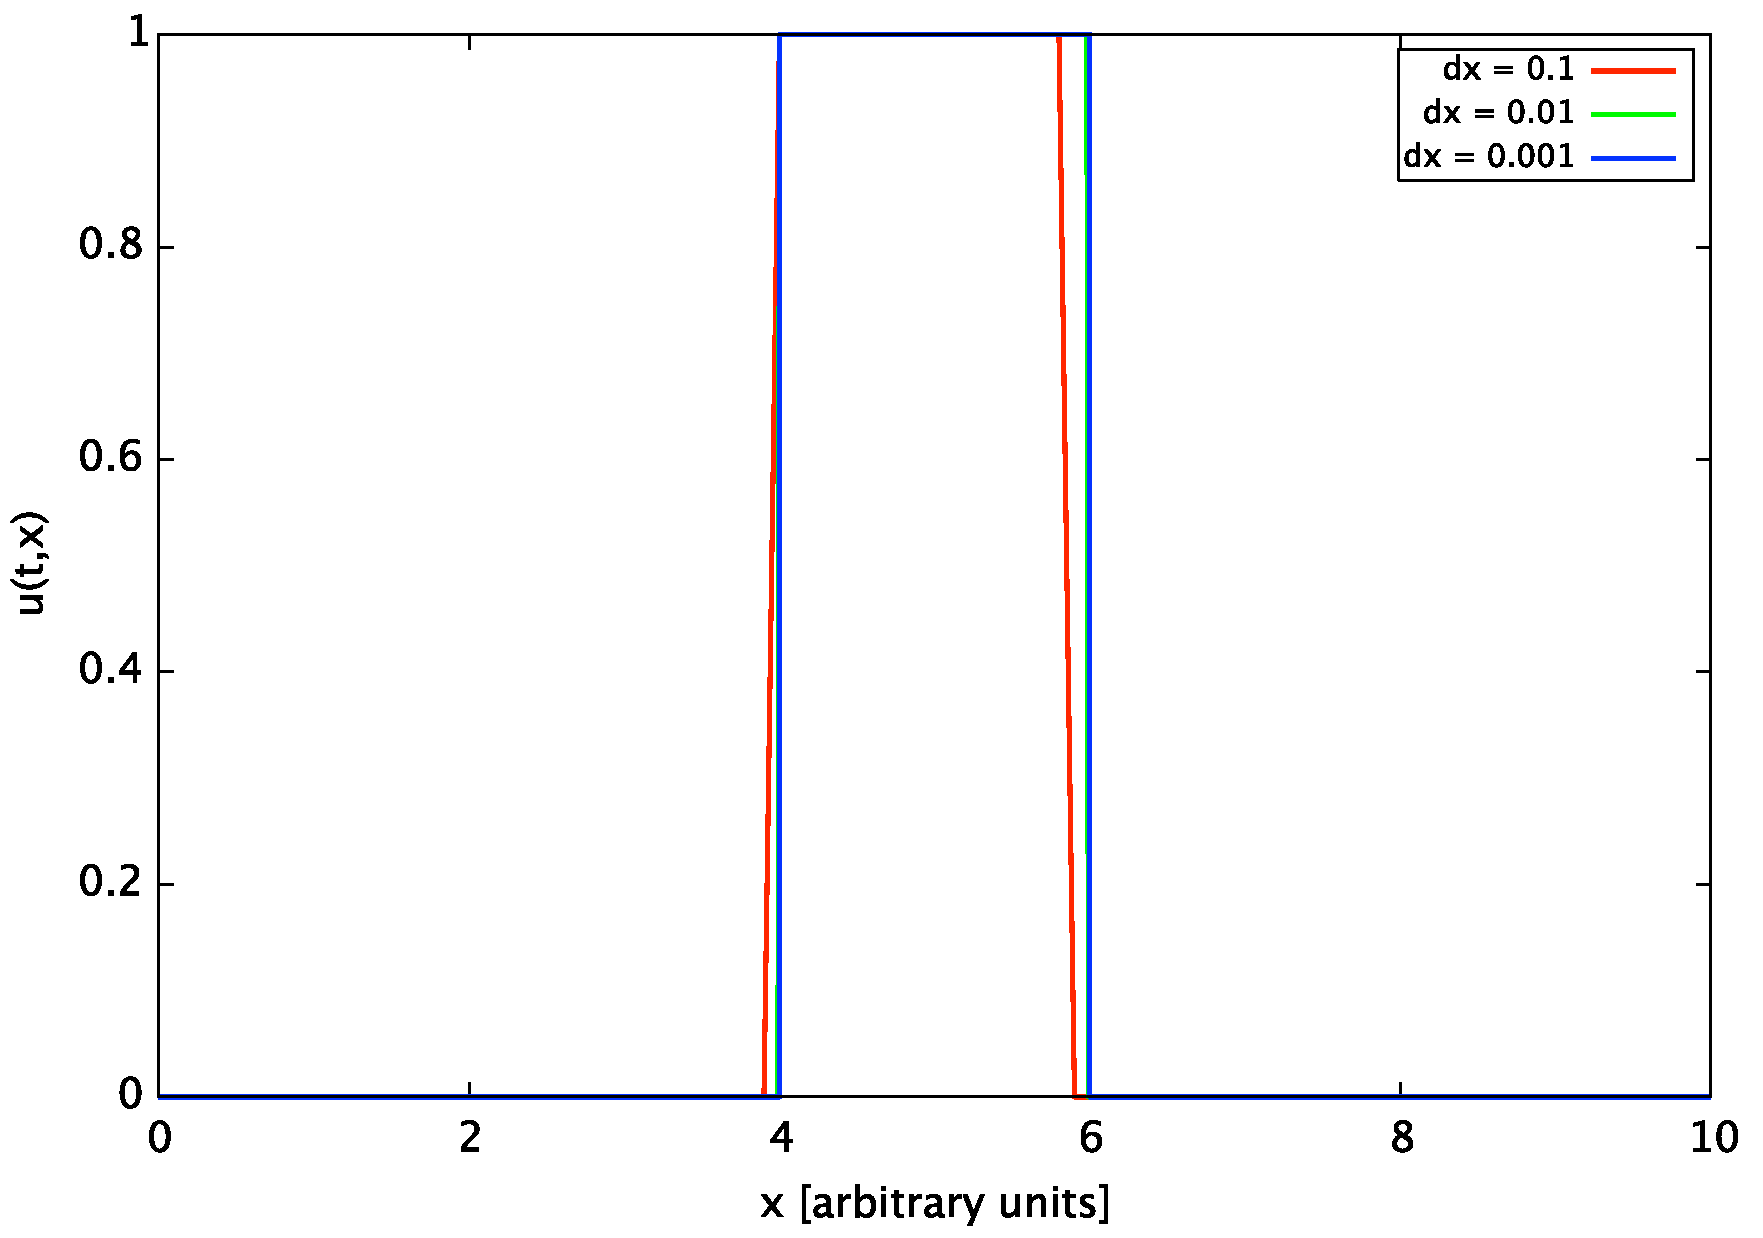
\includegraphics[scale=0.25]{good_img/lxfr_cf1_t10_s} 
\label{fig:first}}
\subfigure[$u(x,t=20)$ with $c_f=1$]{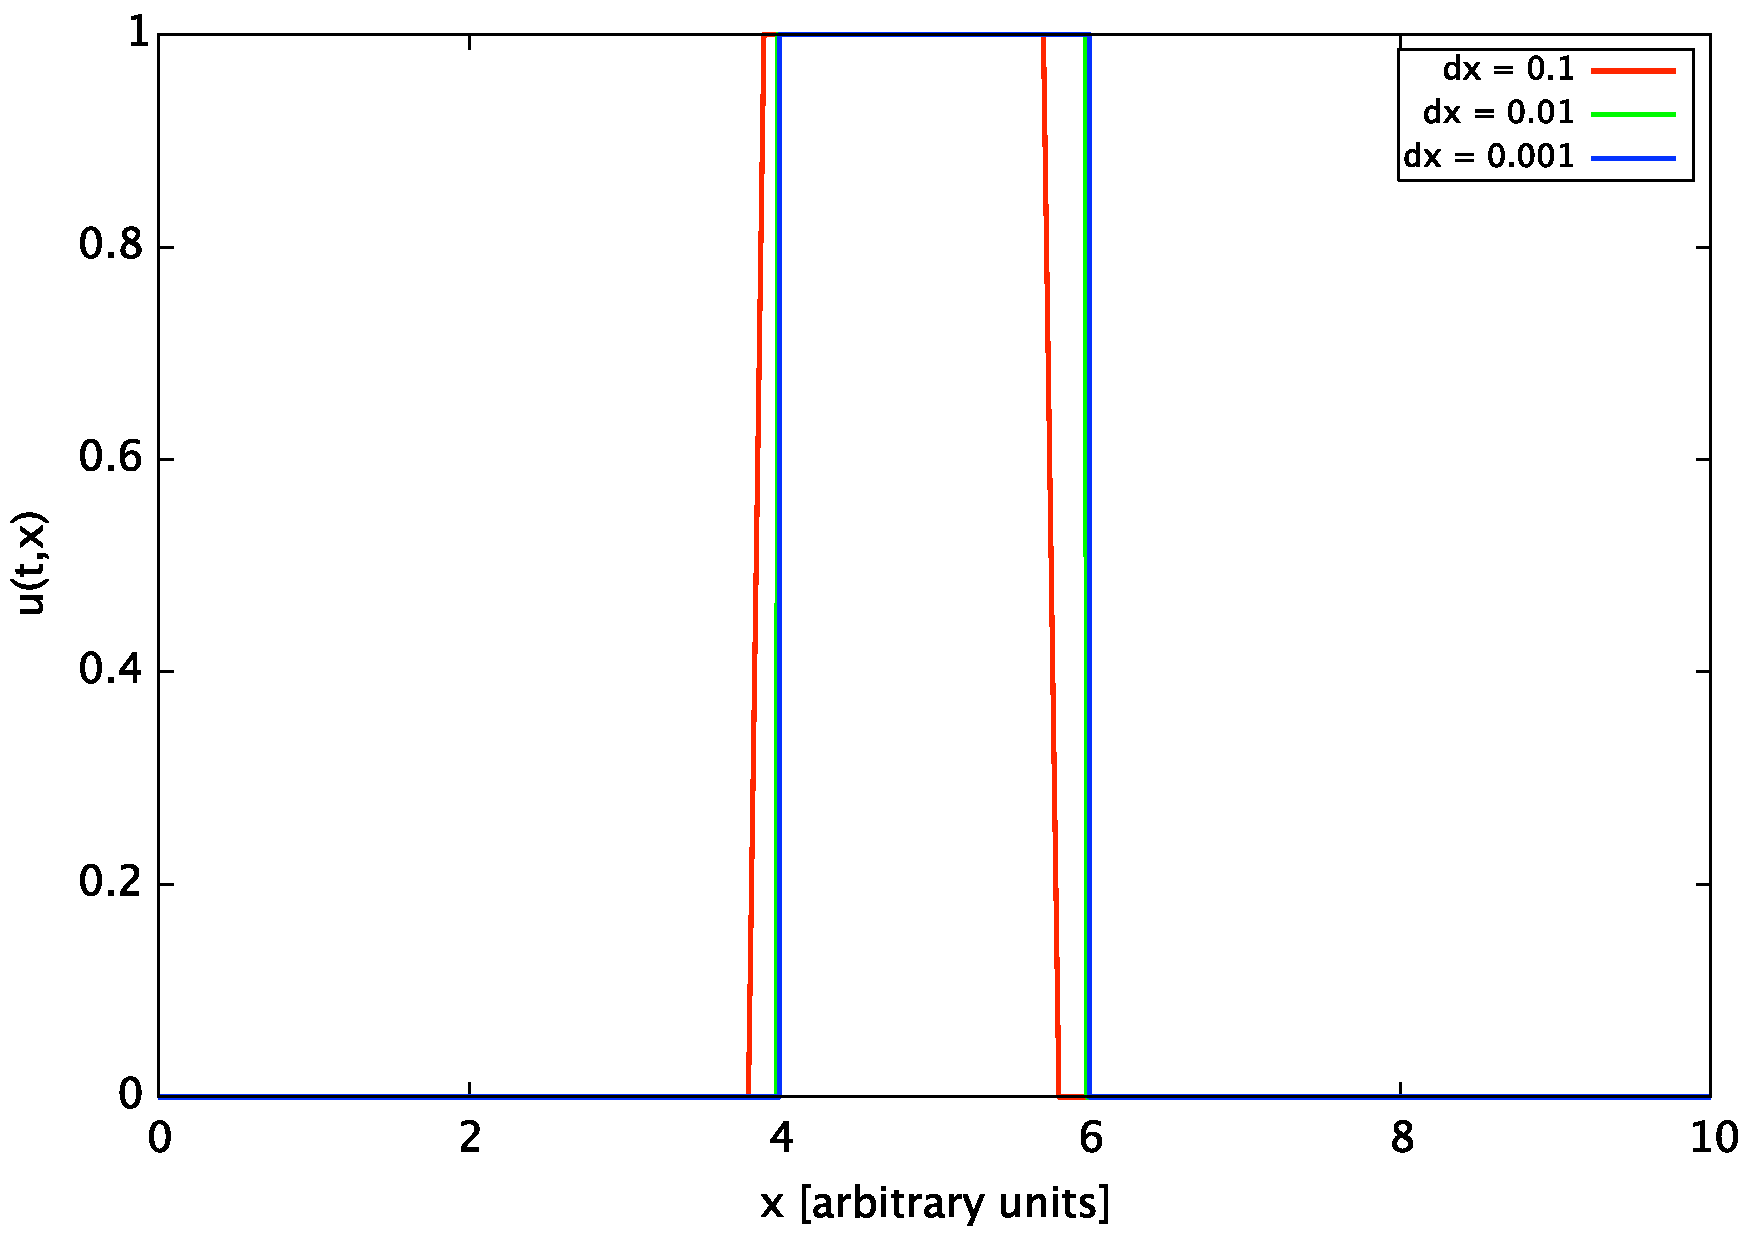
\includegraphics[scale=0.25]{good_img/lxfr_cf1_t20_s}
\label{fig:second}}
\end{center}
\end{figure}\\
The plot of the L2-norms is shown in the following (Fig. 1.37, 1.38). 
\begin{figure}[!h]
\centering
\subfigure[L2-norm with $c_f=0.5$ and $\Delta x = 0.1$ for the Gaussian initial condition]
{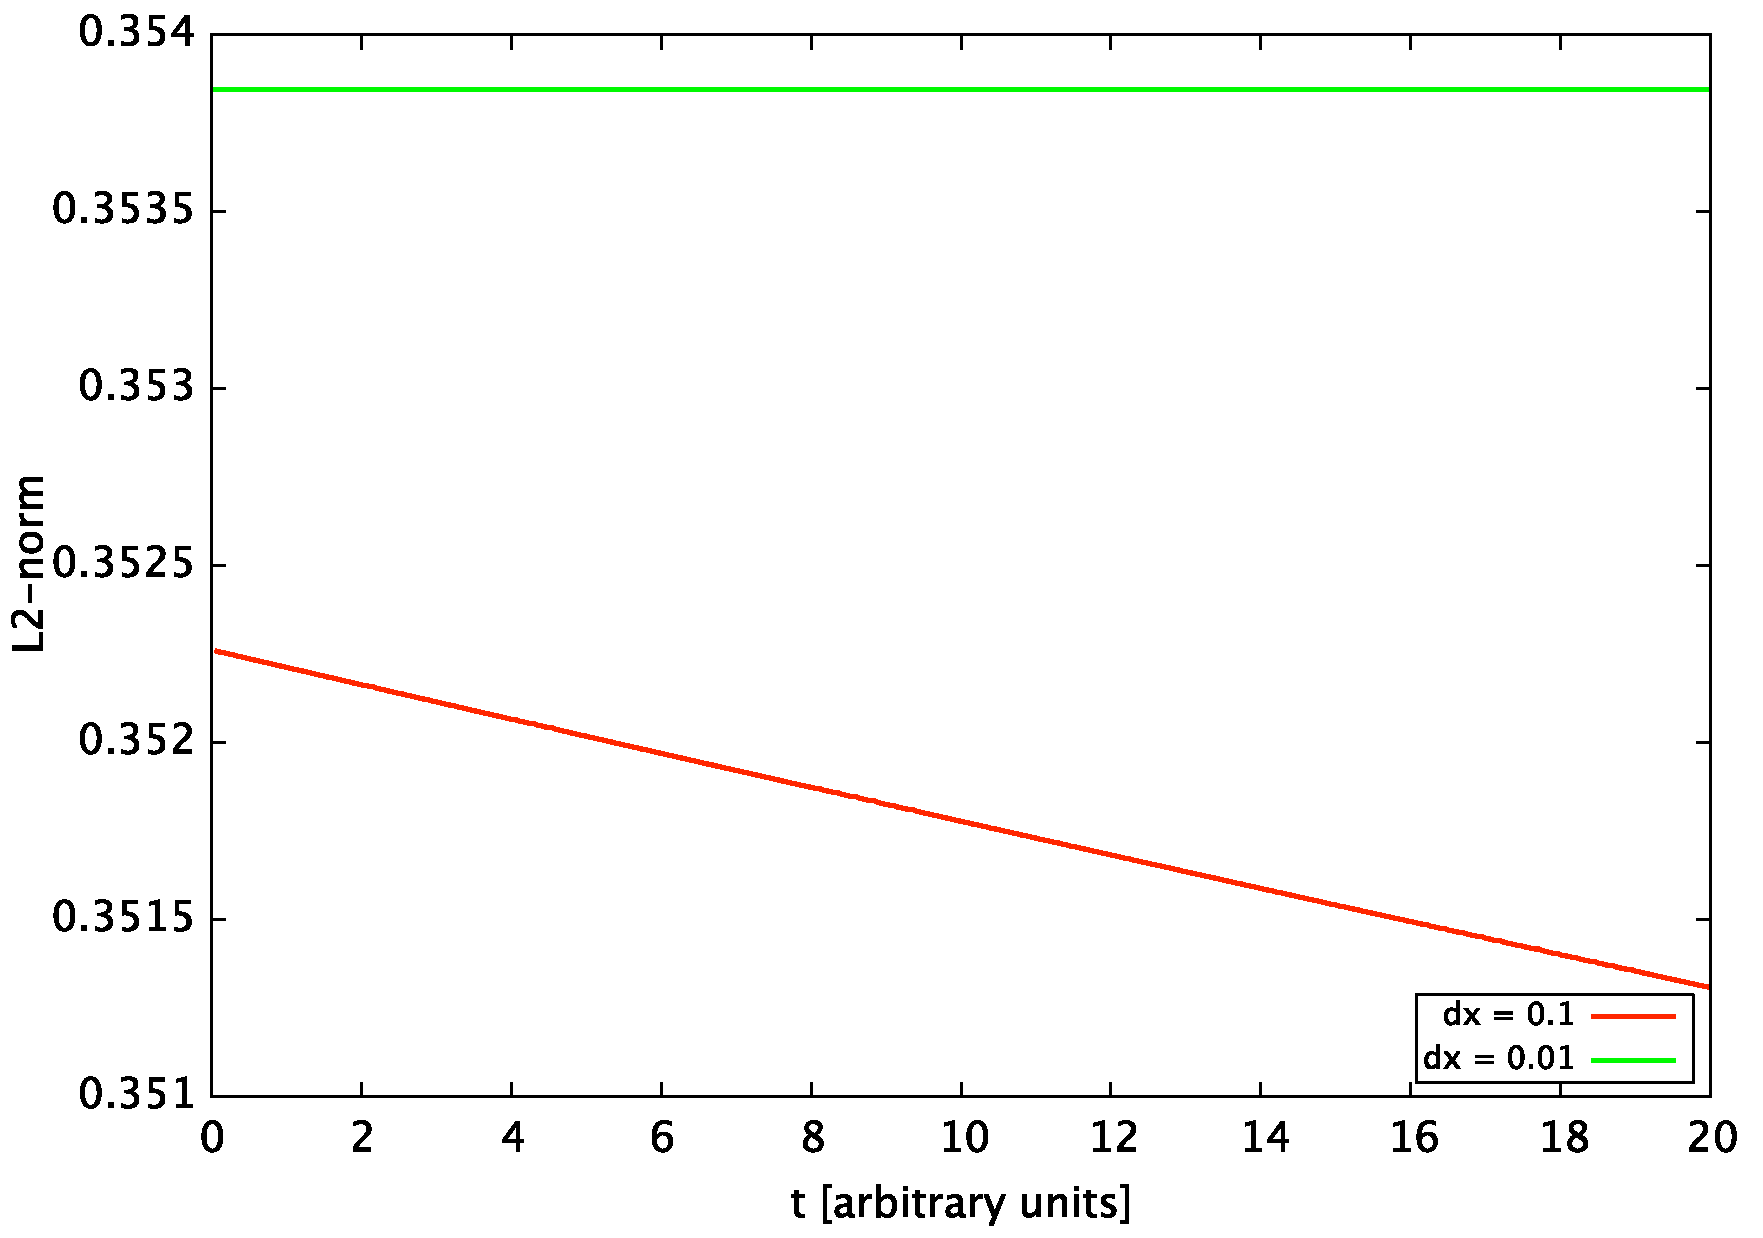
\includegraphics[scale=0.25]{good_img/lw_l2_g}}
\subfigure[L2-norm with $c_f=0.5$ and $\Delta x = 0.1$ for the square wave initial condition]
{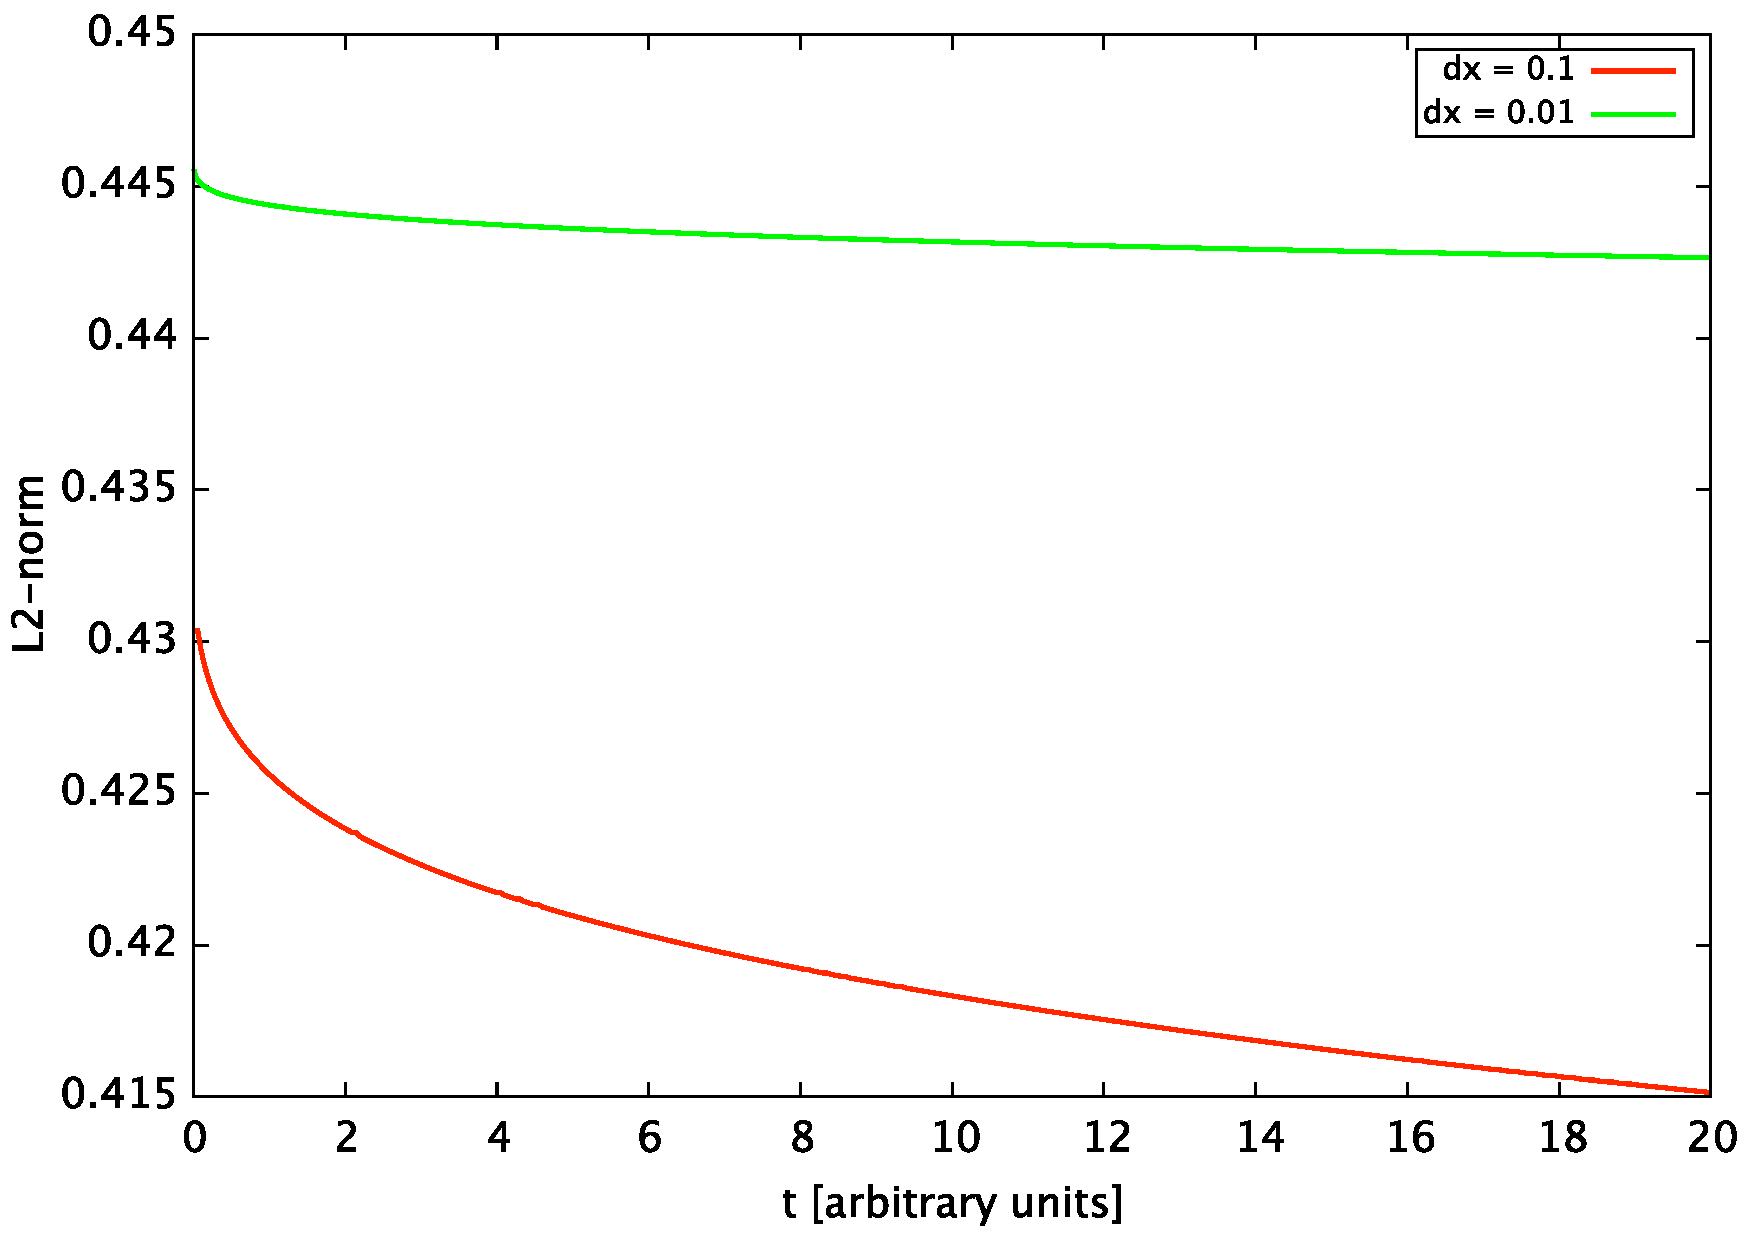
\includegraphics[scale=0.25]{good_img/lw_l2_s}}
\end{figure}
\section{Wave equation}
The wave equation is given by the following second order partial differential equation
\begin{equation}
u_{tt} = v^2 u_{xx}
\end{equation}
where $v$ is a constant. To solve it, it is useful to define two auxiliary functions $s$ and $r$ such that
\begin{equation}
\begin{cases}
r = vu_x \\
s = u_t
\end{cases}
\end{equation}
One sees that
 \[
 \begin{cases}
r_t = vu_{xt} = vu_{tx} = vs_x \\
s_t = u_{tt} = v^2 u_{xx} = vr_x
\end{cases}
 \]
expressions that lead to the following set of coupled first order partial differential equations
\begin{equation}
 \begin{cases}
r_t -vs_x = 0 \\
s_t -  vr_x = 0
\end{cases}
\end{equation}
which are evidently two advection equations. In the following we are going to use the Lax-Friedrichs and Lax-Wendroff algorithms with periodic boundary conditions to solve the wave equation. Let's discuss them. The Lax-Wendroff algorithm is given by
\begin{equation}
 \begin{cases}
r_j^{n+1} = r^n_j + \frac{v \Delta t}{2 \Delta x} \left( s_{j+1}^n - s_{j-1}^n \right) + \frac{v^2 \Delta t^2}{2 \Delta x^2} ( r^n_{j+1} - 2r_j^n + r_{j-1}^n ) \\
s_j^{n+1} = s^n_j + \frac{v \Delta t}{2 \Delta x} \left( r_{j+1}^n - r_{j-1}^n \right) + \frac{v^2 \Delta t^2}{2 \Delta x^2} ( s^n_{j+1} - 2s_j^n + s_{j-1}^n ) 
\end{cases}
\end{equation}
and
\begin{equation}
u_j^{n+1} = u_j^n + \frac{\Delta t}{2} ( s_j^{n+1} + s_j^n )
\end{equation}
while the leapfrog algorithm states
\begin{equation}
 \begin{cases}
r_j^{n+1} = \frac{1}{2}(r_{j+1}^n + r_{j-1}^n) + \frac{\Delta t}{2 \Delta x}(s_{j+1}^n + s_{j-1}^n) \\
s_j^{n+1} = \frac{1}{2}(s_{j+1}^n + s_{j-1}^n) + \frac{\Delta t}{2 \Delta x}(r_{j+1}^n + r_{j-1}^n)
\end{cases}
\end{equation}
and
\begin{equation}
u_j^{n+1} = u_j^n + \frac{\Delta t}{2} ( s_j^{n+1} + s_j^n )
\end{equation}
In the following the results obtained with the two methods for $c_f = 0.5$, different spatial steps and different evolution times are shown (Fig. 1.39 - 1.42)
\begin{figure}[!h]
\centering
\subfigure[$u(x,t=2)$ with $c_f=0.5$]
{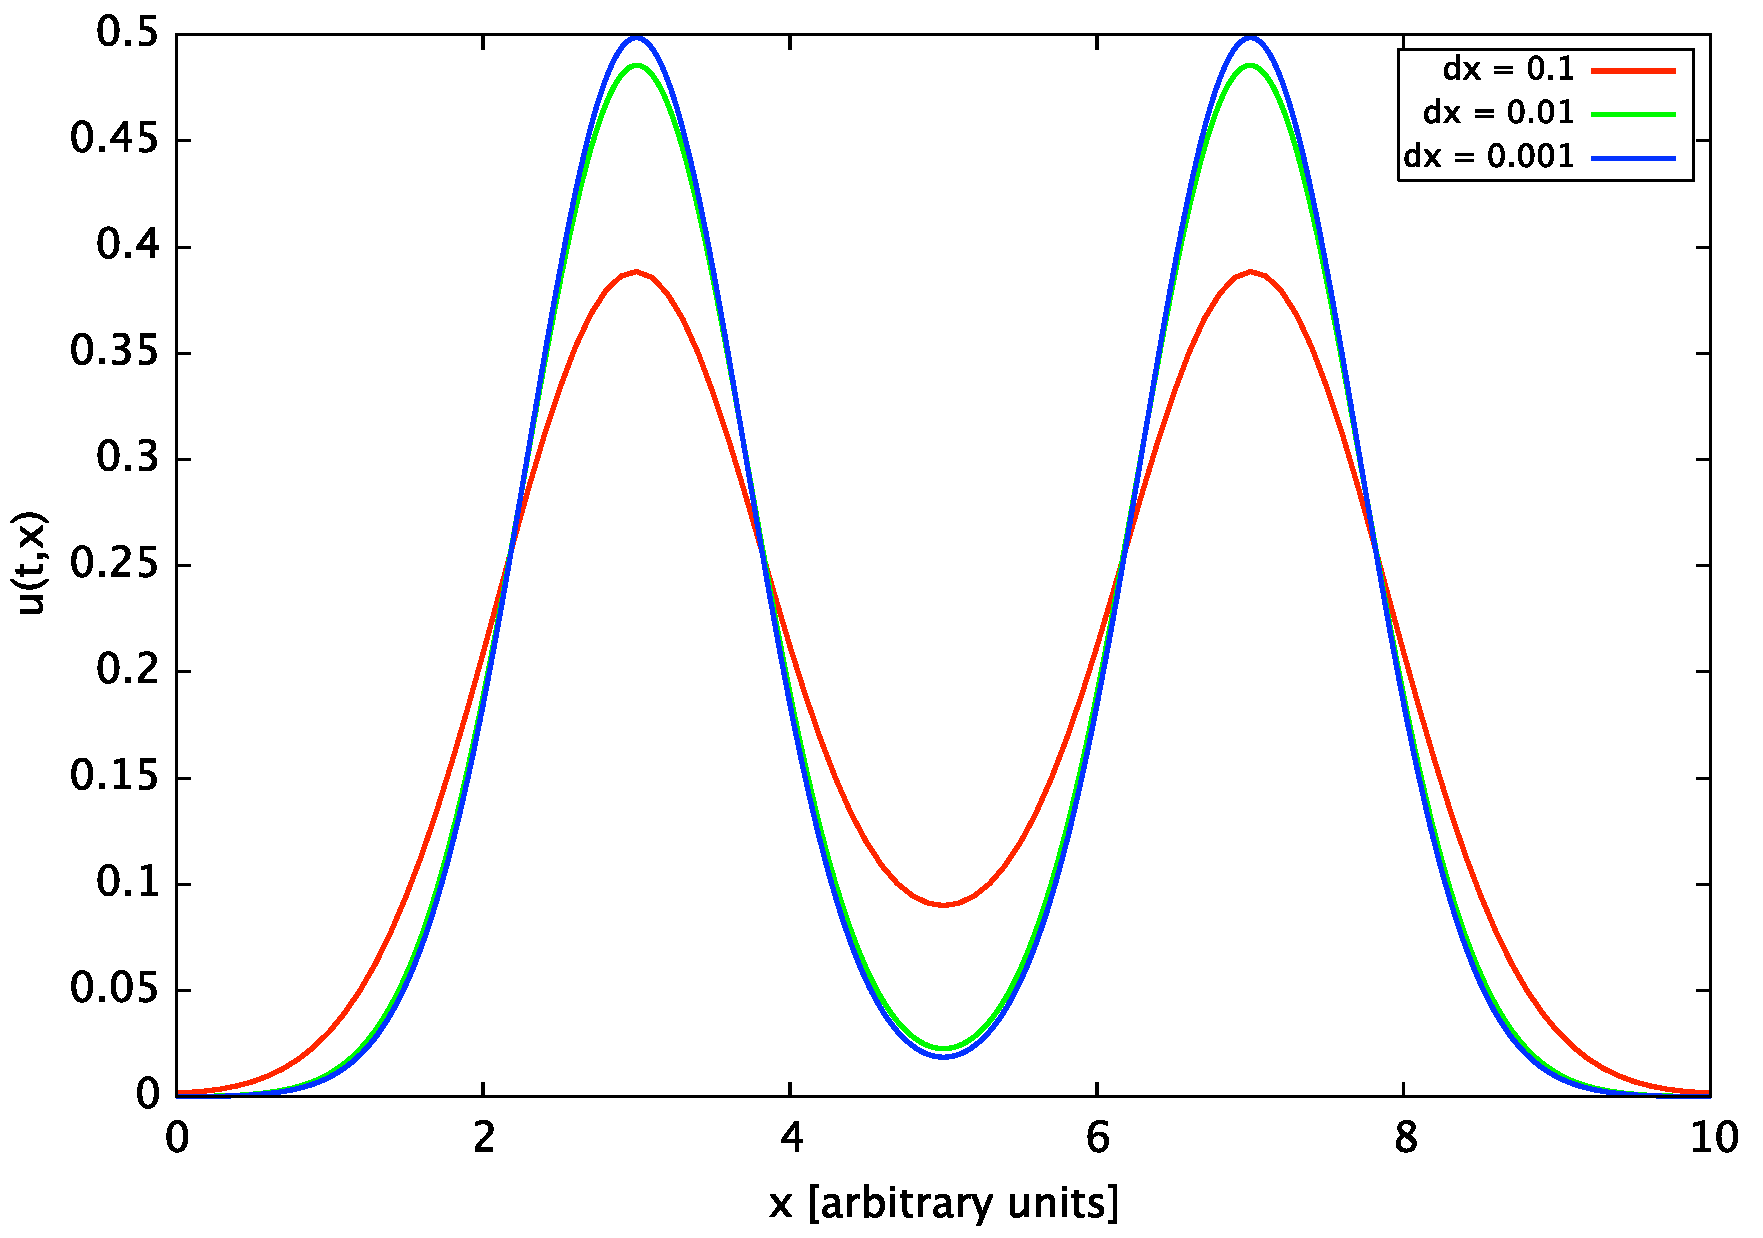
\includegraphics[scale=0.25]{good_img/lefrw_cf05_t2}}
\subfigure[$u(x,t=12)$ with $c_f=0.5$]
{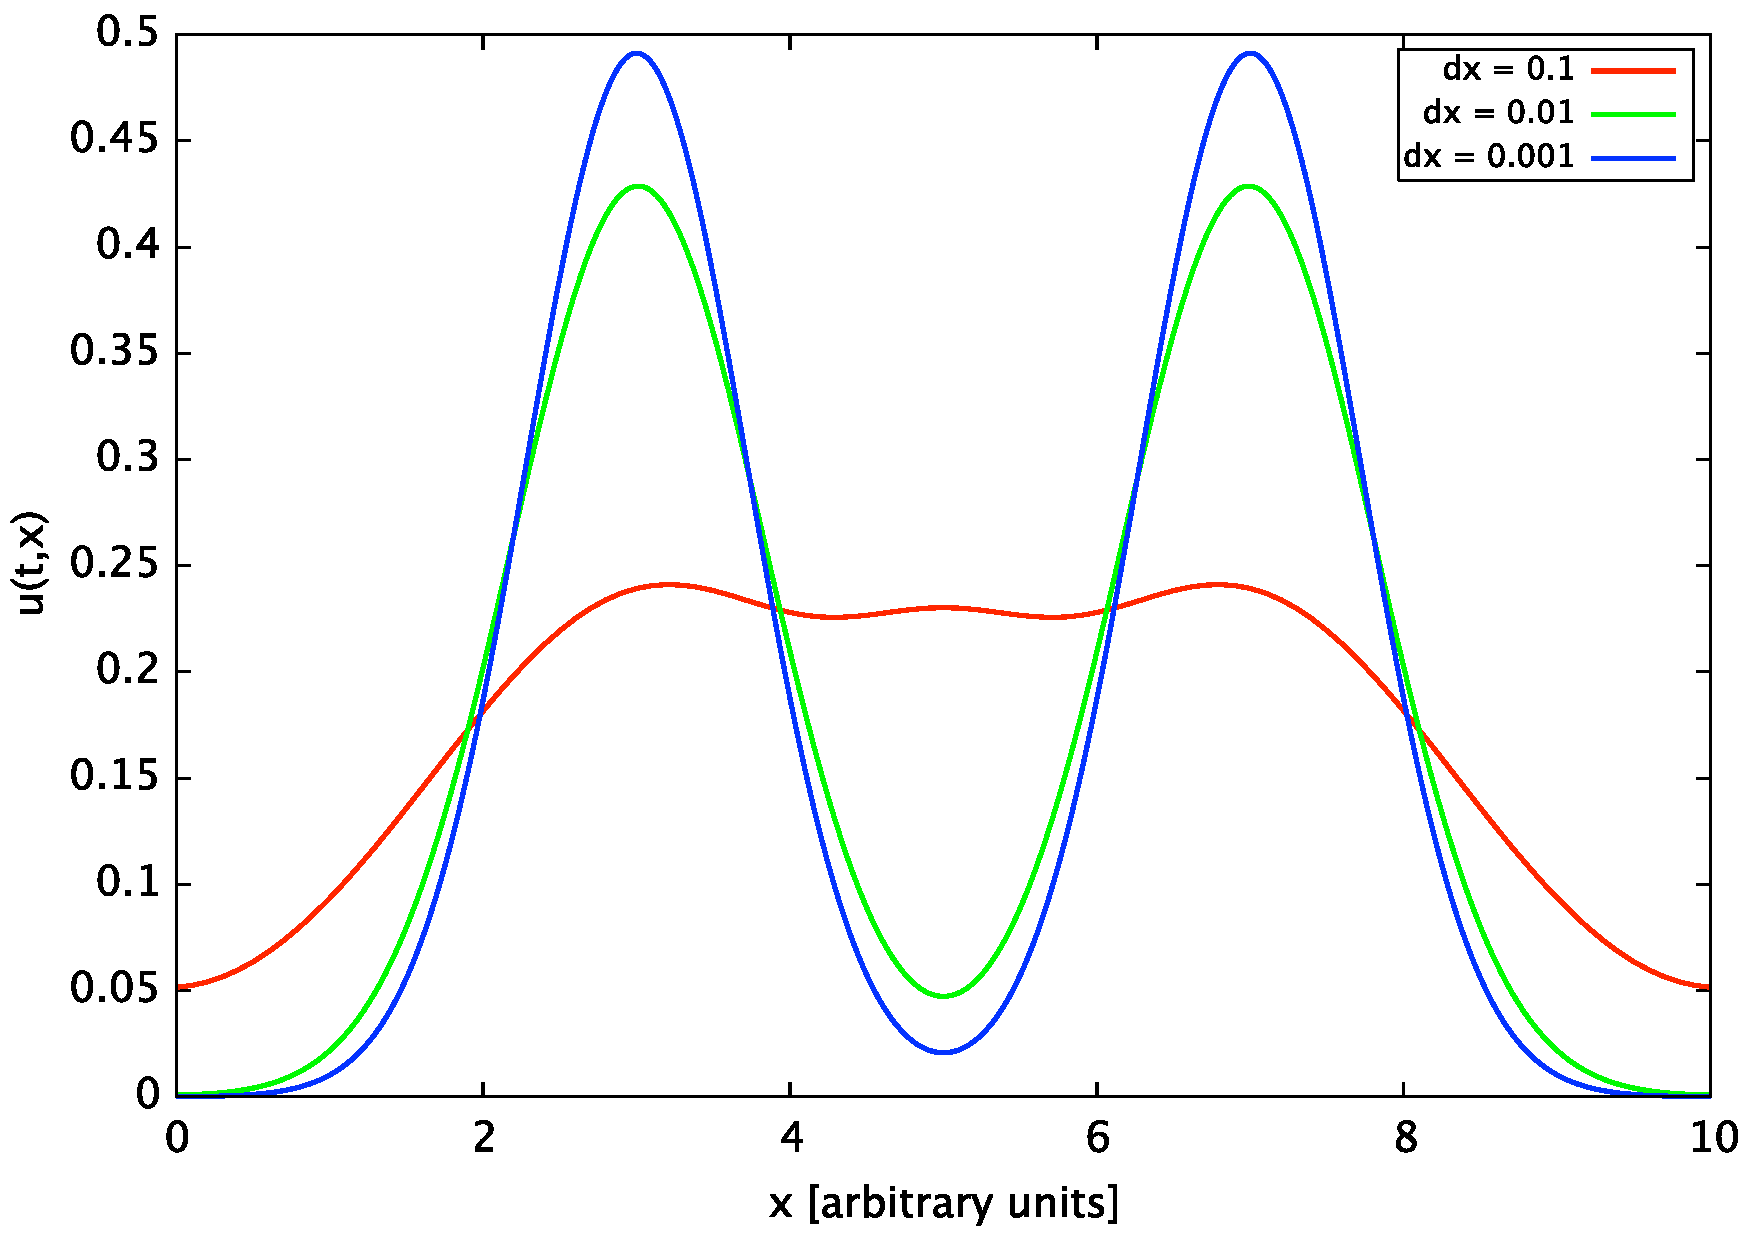
\includegraphics[scale=0.25]{good_img/lefrw_cf05_t12}}
\end{figure}\\
\begin{figure}[!h]
\begin{center}
\subfigure[$u(x,t=2)$ with $c_f=0.5$]{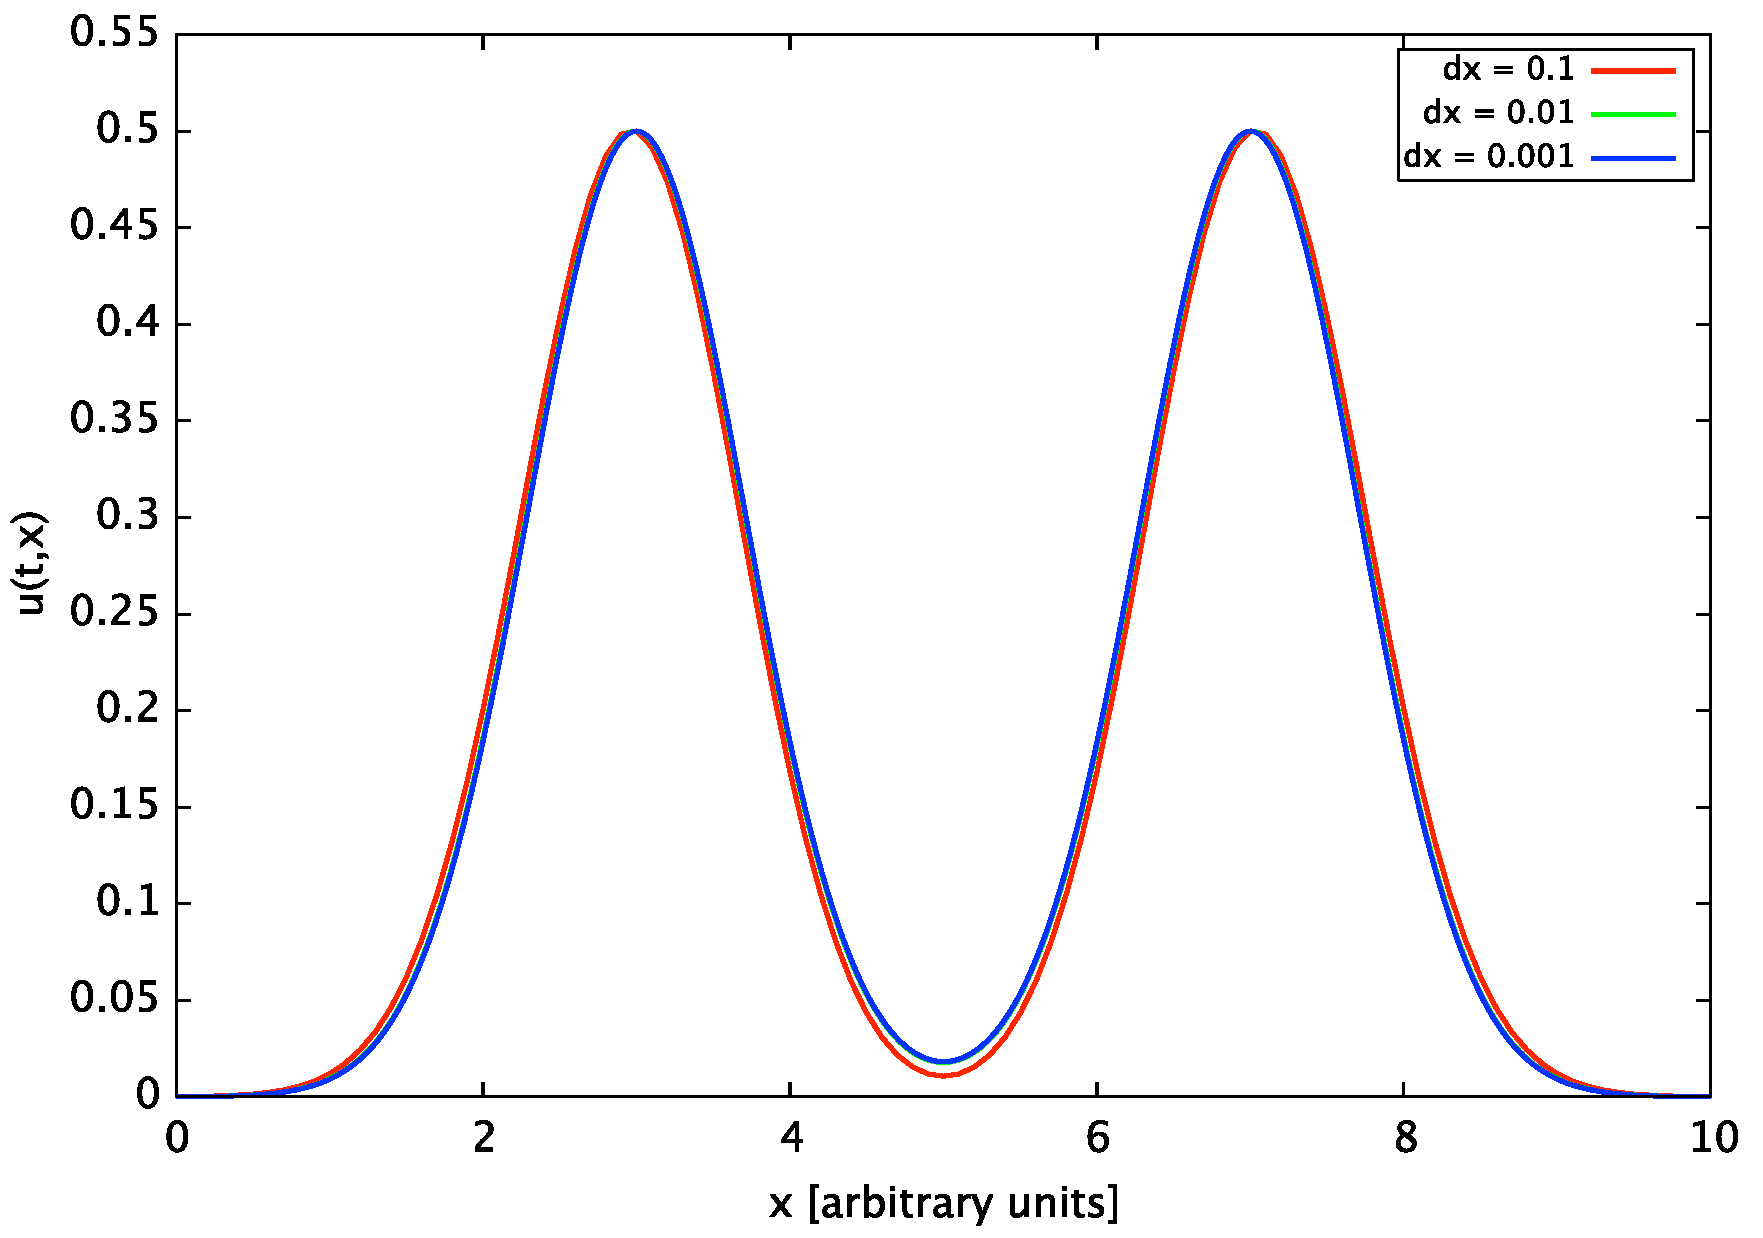
\includegraphics[scale=0.25]{good_img/lww_cf05_t2} 
\label{fig:first}}
\subfigure[$u(x,t=12)$ with $c_f=0.5$]{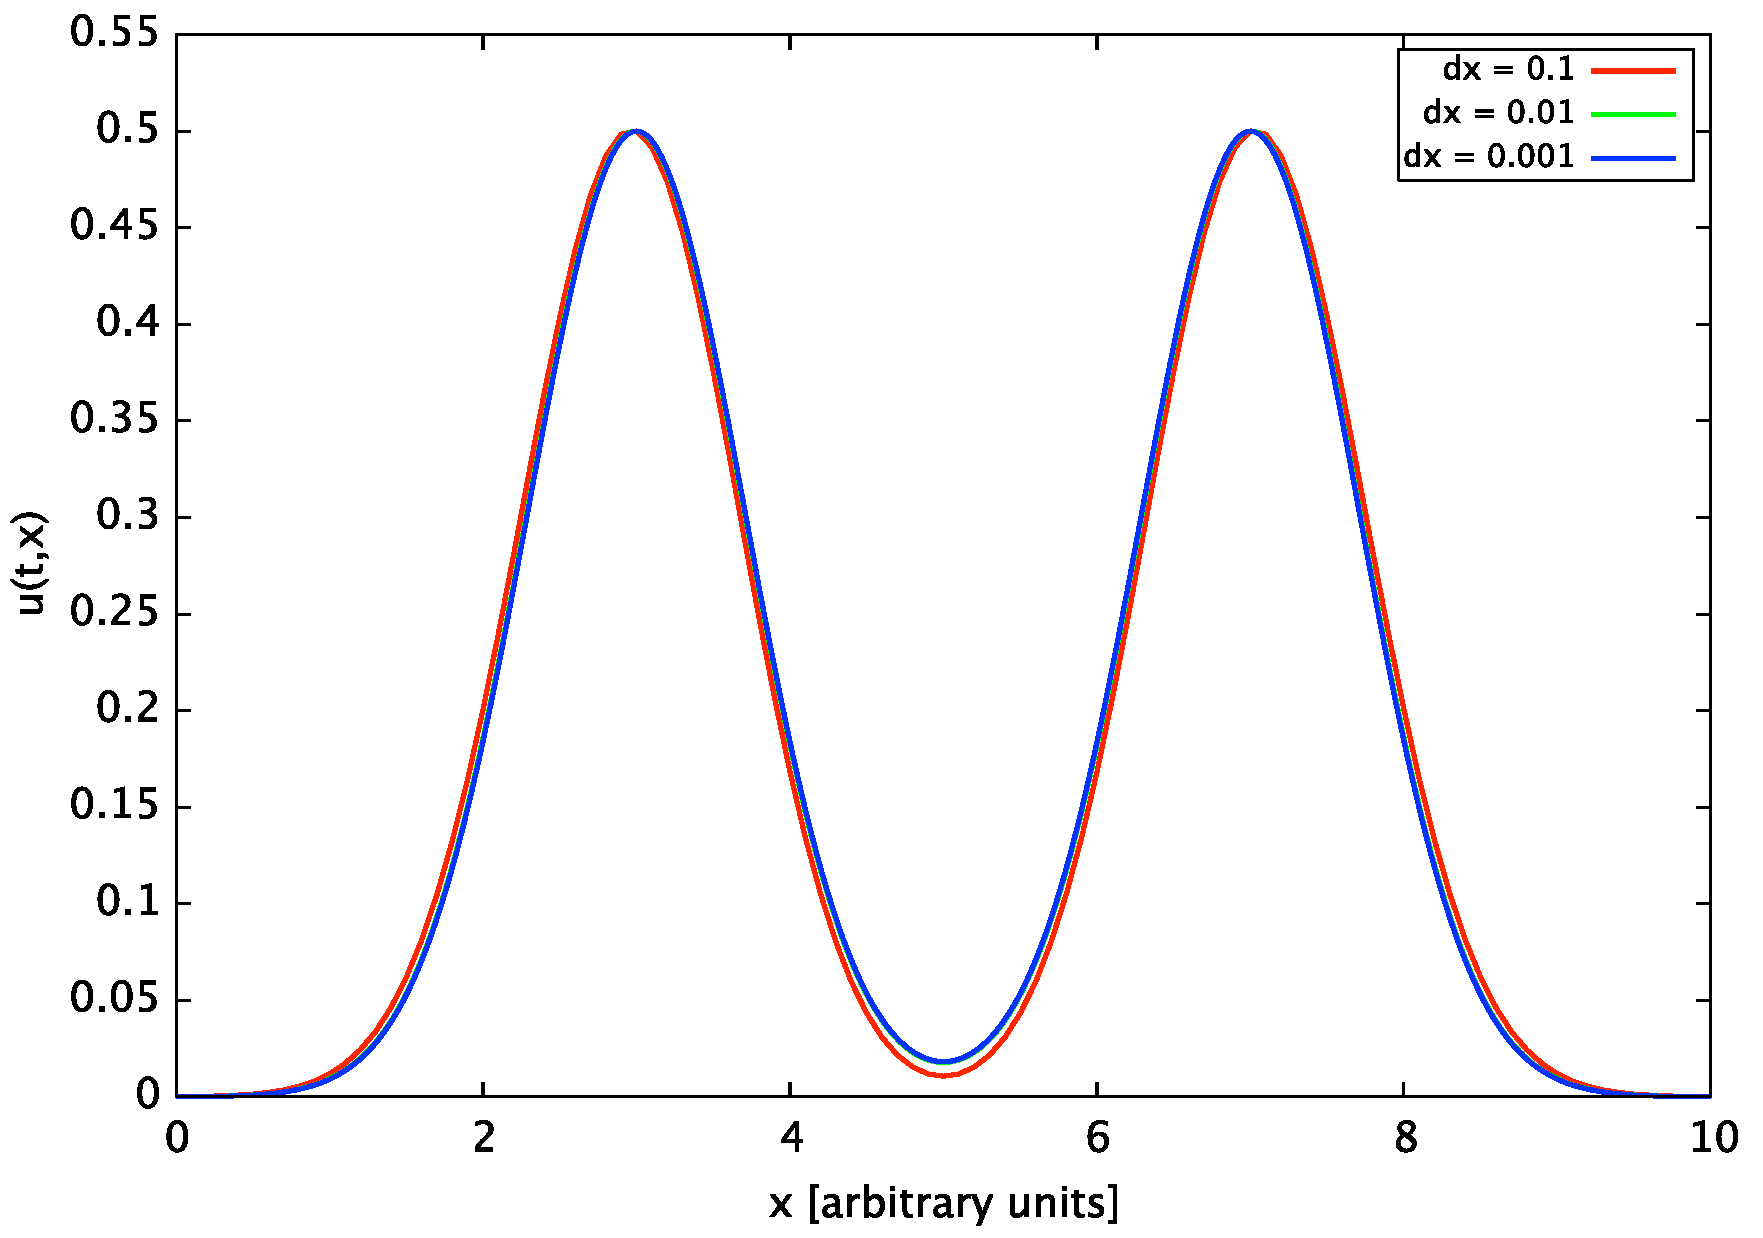
\includegraphics[scale=0.25]{good_img/lww_cf05_t2}
\label{fig:second}}
\subfigure[L2-norm with $c_f=0.5$ for the Lax-Friedrichs method]{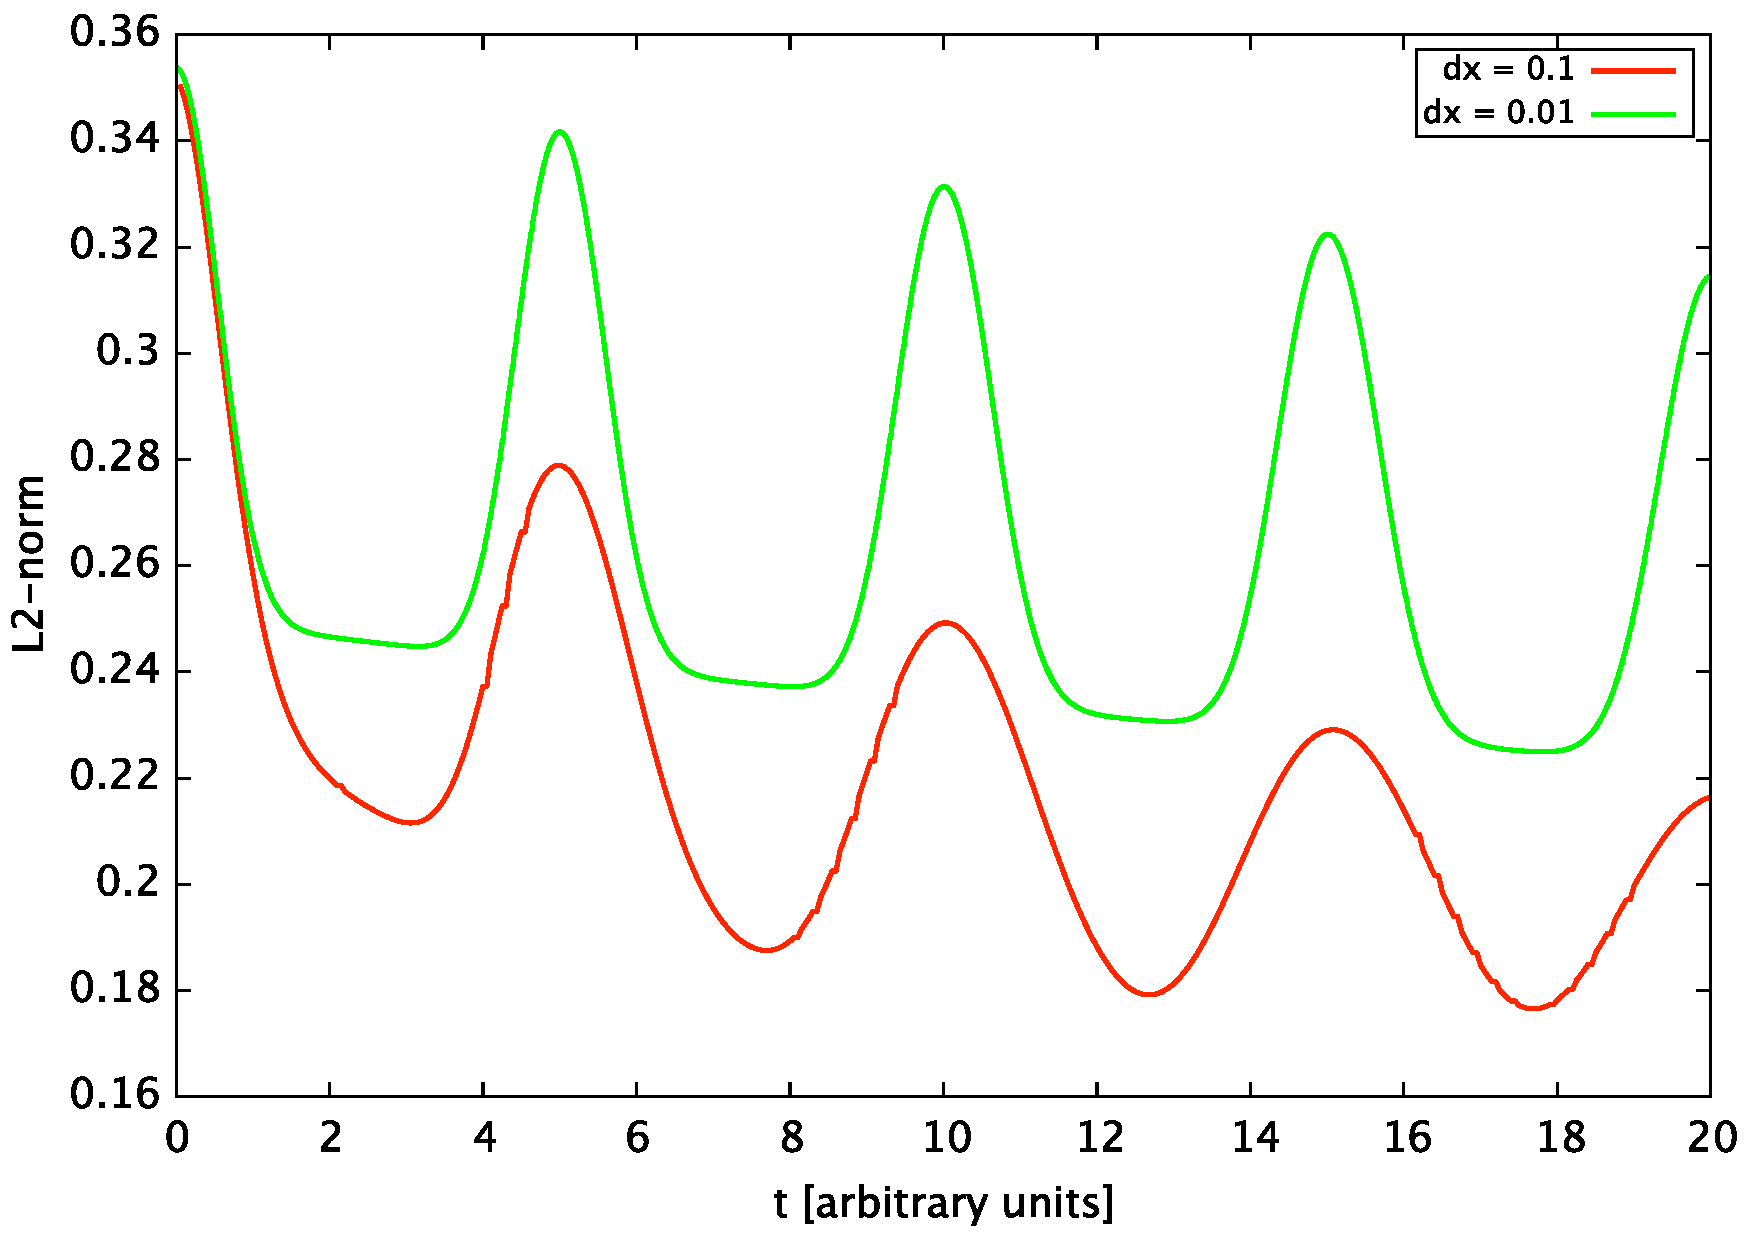
\includegraphics[scale=0.25]{good_img/lefrw_l2} 
\label{fig:first}}
\subfigure[L2-norm with $c_f=0.5$ for the Lax-Wendroff method]{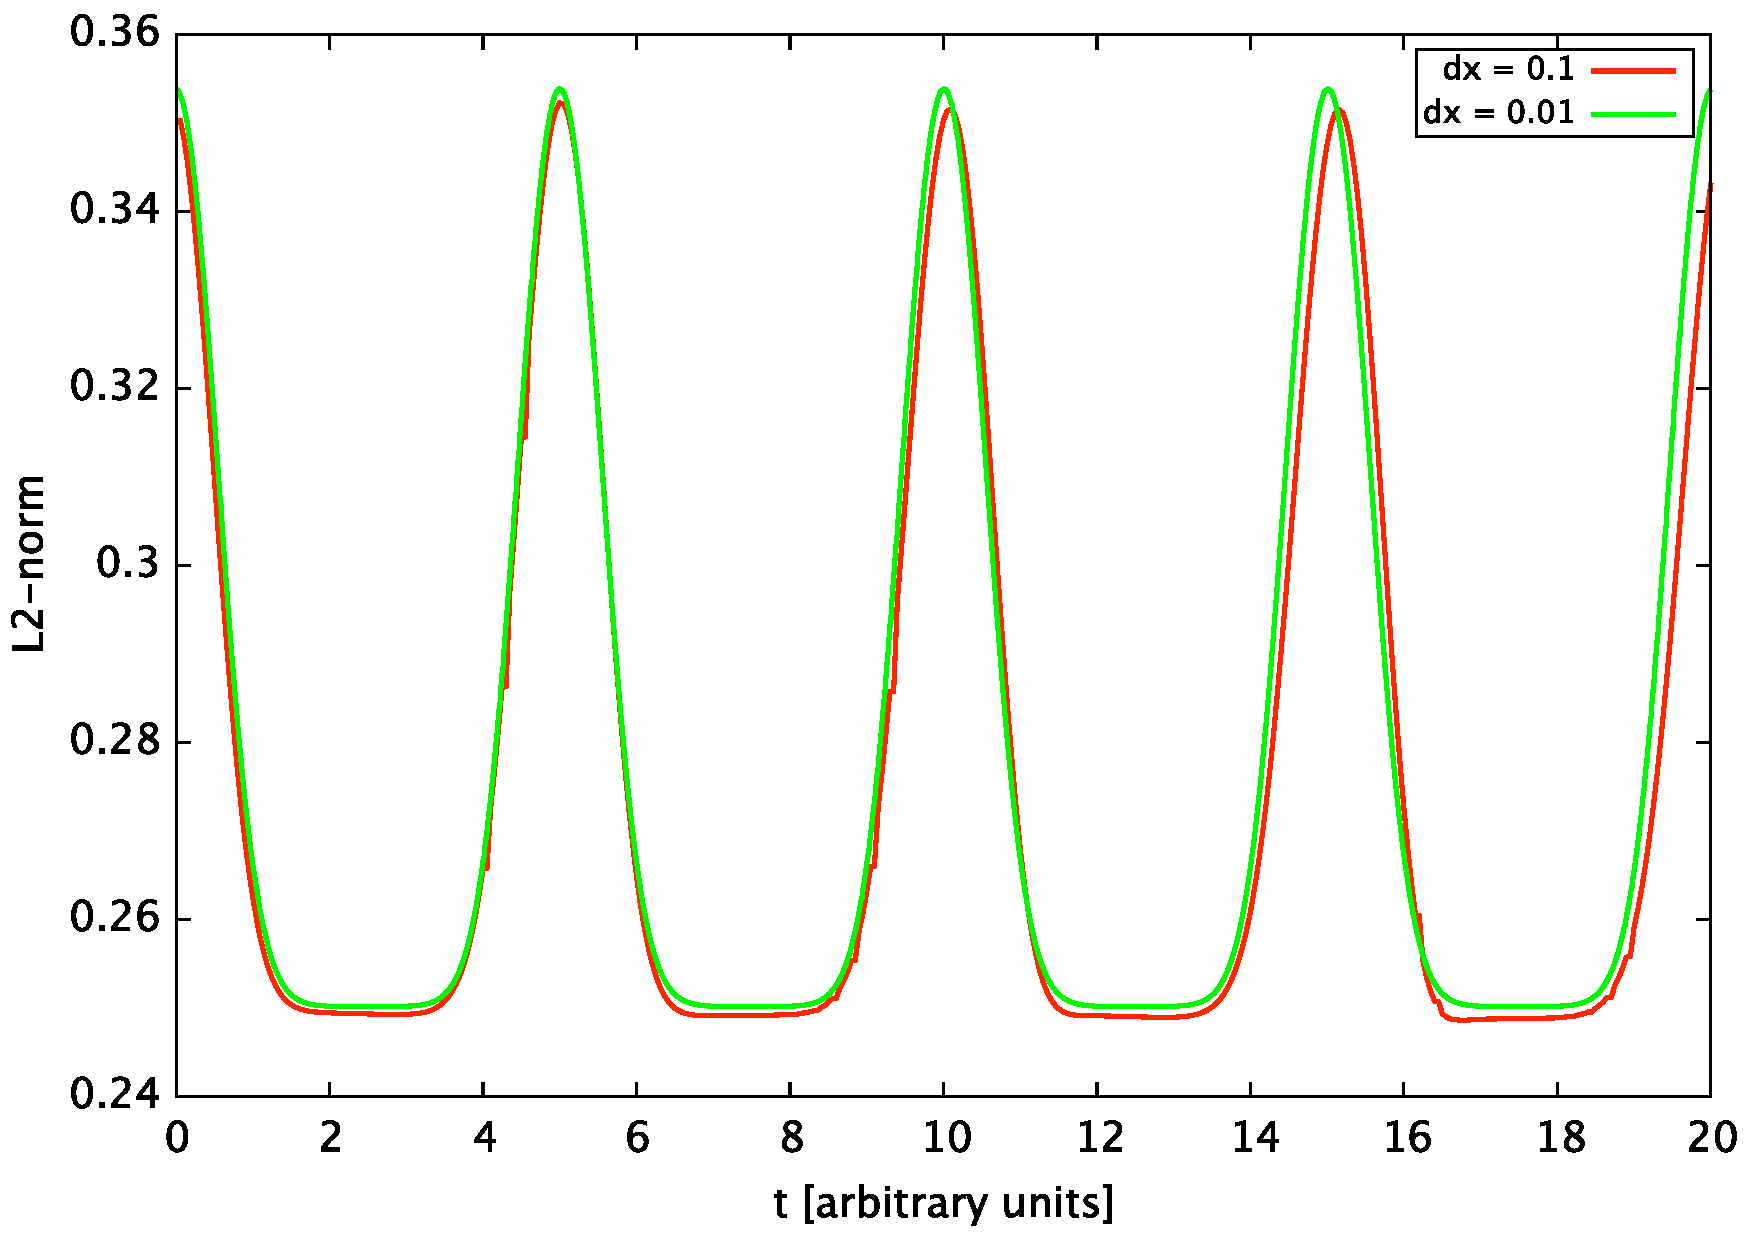
\includegraphics[scale=0.25]{good_img/lww_l2}
\label{fig:second}}
\end{center}
\end{figure}\\
The dispersive behaviour of the Lax-Friedrichs algorithm is particularly evident for $\Delta x \geq 0.01$, where the wavepacket spreads during its time evolution. The same problem is totally absent in Lax-Wendroff, where the time evolution is coherent with the expected behaviour for every space step $\Delta x \leq 0.1$. Finally, the L2-norms are shown in Fig. 1.43, 1.44. 

\end{document}